% Options for packages loaded elsewhere
% Options for packages loaded elsewhere
\PassOptionsToPackage{unicode}{hyperref}
\PassOptionsToPackage{hyphens}{url}
\PassOptionsToPackage{dvipsnames,svgnames,x11names}{xcolor}
%
\documentclass[
  10pt,
]{article}
\usepackage{xcolor}
\usepackage{amsmath,amssymb}
\setcounter{secnumdepth}{5}
\usepackage{iftex}
\ifPDFTeX
  \usepackage[T1]{fontenc}
  \usepackage[utf8]{inputenc}
  \usepackage{textcomp} % provide euro and other symbols
\else % if luatex or xetex
  \usepackage{unicode-math} % this also loads fontspec
  \defaultfontfeatures{Scale=MatchLowercase}
  \defaultfontfeatures[\rmfamily]{Ligatures=TeX,Scale=1}
\fi
\usepackage{lmodern}
\ifPDFTeX\else
  % xetex/luatex font selection
\fi
% Use upquote if available, for straight quotes in verbatim environments
\IfFileExists{upquote.sty}{\usepackage{upquote}}{}
\IfFileExists{microtype.sty}{% use microtype if available
  \usepackage[]{microtype}
  \UseMicrotypeSet[protrusion]{basicmath} % disable protrusion for tt fonts
}{}
\makeatletter
\@ifundefined{KOMAClassName}{% if non-KOMA class
  \IfFileExists{parskip.sty}{%
    \usepackage{parskip}
  }{% else
    \setlength{\parindent}{0pt}
    \setlength{\parskip}{6pt plus 2pt minus 1pt}}
}{% if KOMA class
  \KOMAoptions{parskip=half}}
\makeatother
% Make \paragraph and \subparagraph free-standing
\makeatletter
\ifx\paragraph\undefined\else
  \let\oldparagraph\paragraph
  \renewcommand{\paragraph}{
    \@ifstar
      \xxxParagraphStar
      \xxxParagraphNoStar
  }
  \newcommand{\xxxParagraphStar}[1]{\oldparagraph*{#1}\mbox{}}
  \newcommand{\xxxParagraphNoStar}[1]{\oldparagraph{#1}\mbox{}}
\fi
\ifx\subparagraph\undefined\else
  \let\oldsubparagraph\subparagraph
  \renewcommand{\subparagraph}{
    \@ifstar
      \xxxSubParagraphStar
      \xxxSubParagraphNoStar
  }
  \newcommand{\xxxSubParagraphStar}[1]{\oldsubparagraph*{#1}\mbox{}}
  \newcommand{\xxxSubParagraphNoStar}[1]{\oldsubparagraph{#1}\mbox{}}
\fi
\makeatother


\usepackage{longtable,booktabs,array}
\usepackage{calc} % for calculating minipage widths
% Correct order of tables after \paragraph or \subparagraph
\usepackage{etoolbox}
\makeatletter
\patchcmd\longtable{\par}{\if@noskipsec\mbox{}\fi\par}{}{}
\makeatother
% Allow footnotes in longtable head/foot
\IfFileExists{footnotehyper.sty}{\usepackage{footnotehyper}}{\usepackage{footnote}}
\makesavenoteenv{longtable}
\usepackage{graphicx}
\makeatletter
\newsavebox\pandoc@box
\newcommand*\pandocbounded[1]{% scales image to fit in text height/width
  \sbox\pandoc@box{#1}%
  \Gscale@div\@tempa{\textheight}{\dimexpr\ht\pandoc@box+\dp\pandoc@box\relax}%
  \Gscale@div\@tempb{\linewidth}{\wd\pandoc@box}%
  \ifdim\@tempb\p@<\@tempa\p@\let\@tempa\@tempb\fi% select the smaller of both
  \ifdim\@tempa\p@<\p@\scalebox{\@tempa}{\usebox\pandoc@box}%
  \else\usebox{\pandoc@box}%
  \fi%
}
% Set default figure placement to htbp
\def\fps@figure{htbp}
\makeatother


% definitions for citeproc citations
\NewDocumentCommand\citeproctext{}{}
\NewDocumentCommand\citeproc{mm}{%
  \begingroup\def\citeproctext{#2}\cite{#1}\endgroup}
\makeatletter
 % allow citations to break across lines
 \let\@cite@ofmt\@firstofone
 % avoid brackets around text for \cite:
 \def\@biblabel#1{}
 \def\@cite#1#2{{#1\if@tempswa , #2\fi}}
\makeatother
\newlength{\cslhangindent}
\setlength{\cslhangindent}{1.5em}
\newlength{\csllabelwidth}
\setlength{\csllabelwidth}{3em}
\newenvironment{CSLReferences}[2] % #1 hanging-indent, #2 entry-spacing
 {\begin{list}{}{%
  \setlength{\itemindent}{0pt}
  \setlength{\leftmargin}{0pt}
  \setlength{\parsep}{0pt}
  % turn on hanging indent if param 1 is 1
  \ifodd #1
   \setlength{\leftmargin}{\cslhangindent}
   \setlength{\itemindent}{-1\cslhangindent}
  \fi
  % set entry spacing
  \setlength{\itemsep}{#2\baselineskip}}}
 {\end{list}}
\usepackage{calc}
\newcommand{\CSLBlock}[1]{\hfill\break\parbox[t]{\linewidth}{\strut\ignorespaces#1\strut}}
\newcommand{\CSLLeftMargin}[1]{\parbox[t]{\csllabelwidth}{\strut#1\strut}}
\newcommand{\CSLRightInline}[1]{\parbox[t]{\linewidth - \csllabelwidth}{\strut#1\strut}}
\newcommand{\CSLIndent}[1]{\hspace{\cslhangindent}#1}



\setlength{\emergencystretch}{3em} % prevent overfull lines

\providecommand{\tightlist}{%
  \setlength{\itemsep}{0pt}\setlength{\parskip}{0pt}}



 


\usepackage[margin=1in]{geometry}
\usepackage{tikz}
\usepackage{adjustbox}
\usepackage{placeins}
\usepackage{appendix}
\usepackage{hyperref}
\usepackage{amsmath}
\usepackage{subfig}
\usepackage{booktabs}
\usepackage{longtable}
\usepackage{array}
\usepackage{multirow}
\usepackage{wrapfig}
\usepackage{float}
\usepackage{colortbl}
\usepackage{pdflscape}
\usepackage{tabu}
\usepackage{threeparttable}
\usepackage{threeparttablex}
\usepackage[normalem]{ulem}
\usepackage{makecell}
\usepackage{xcolor}
\makeatletter
\@ifpackageloaded{caption}{}{\usepackage{caption}}
\AtBeginDocument{%
\ifdefined\contentsname
  \renewcommand*\contentsname{Table of contents}
\else
  \newcommand\contentsname{Table of contents}
\fi
\ifdefined\listfigurename
  \renewcommand*\listfigurename{List of Figures}
\else
  \newcommand\listfigurename{List of Figures}
\fi
\ifdefined\listtablename
  \renewcommand*\listtablename{List of Tables}
\else
  \newcommand\listtablename{List of Tables}
\fi
\ifdefined\figurename
  \renewcommand*\figurename{Figure}
\else
  \newcommand\figurename{Figure}
\fi
\ifdefined\tablename
  \renewcommand*\tablename{Table}
\else
  \newcommand\tablename{Table}
\fi
}
\@ifpackageloaded{float}{}{\usepackage{float}}
\floatstyle{ruled}
\@ifundefined{c@chapter}{\newfloat{codelisting}{h}{lop}}{\newfloat{codelisting}{h}{lop}[chapter]}
\floatname{codelisting}{Listing}
\newcommand*\listoflistings{\listof{codelisting}{List of Listings}}
\makeatother
\makeatletter
\makeatother
\makeatletter
\@ifpackageloaded{caption}{}{\usepackage{caption}}
\@ifpackageloaded{subcaption}{}{\usepackage{subcaption}}
\makeatother
\usepackage{bookmark}
\IfFileExists{xurl.sty}{\usepackage{xurl}}{} % add URL line breaks if available
\urlstyle{same}
\hypersetup{
  pdftitle={Uneven Wage Growth and Public Goods},
  pdfauthor={Ebba Mark},
  colorlinks=true,
  linkcolor={blue},
  filecolor={Maroon},
  citecolor={Blue},
  urlcolor={Blue},
  pdfcreator={LaTeX via pandoc}}


\title{Uneven Wage Growth and Public Goods}
\usepackage{etoolbox}
\makeatletter
\providecommand{\subtitle}[1]{% add subtitle to \maketitle
  \apptocmd{\@title}{\par {\large #1 \par}}{}{}
}
\makeatother
\subtitle{The Case of US Public Education}
\author{Ebba Mark}
\date{}
\begin{document}
\maketitle
\begin{abstract}
Over recent decades, the United States has experienced increasingly
divergent patterns of economic and wage growth. Wage growth is a key
driver of local wealth accumulation, enabling greater household and
community investment in public goods. Regions whose wages track
productivity gains likely benefit from broader economic growth,
accumulating wealth that sustains local public services, while lagging
regions risk weaker savings rates and eroding fiscal capacities. We
estimate how divergent wage growth across U.S. regions affects public
education expenditure using a shift-share instrumental variable design.
Accounting for state-level heterogeneity in tax regimes, income, and
economic growth, we find substantial variation in the elasticity of
education spending to wages: the magnitude and statistical significance
differ markedly across states. This heterogeneity explains the majority
of spending responses and reflects both uneven economic fundamentals and
diverse fiscal institutions that generate inequality in public goods
provision. Our results demonstrate that average treatment effects in
panel studies can obscure critical policy-relevant variation. The
findings suggest that federal and local policies assuming uniform
wage-spending relationships may fail to address or even exacerbate
pervasive spatial inequality in educational investment.
\end{abstract}

\renewcommand*\contentsname{Table of contents}
{
\hypersetup{linkcolor=}
\setcounter{tocdepth}{3}
\tableofcontents
}

\section{Introduction}\label{introduction}

\textbf{Since the 1970s, a persistent divergence between productivity
growth and wage growth has emerged in the United States ( Hoffmann, Lee,
and Lemieux (2020), Stansbury and Summers (n.d.), Economic Policy
Institute (n.d.)).} While labour productivity has continued to rise, the
earnings of typical workers have increased far more slowly, leading to a
substantial decoupling between the two trends. Economists cite various
contributors to this phenomenon from human capital (Autor (2014), Katz
and Murphy (1992)) to competition (Stansbury and Summers (n.d.), Deb et
al. (2022), Yeh, Macaluso, and Hershbein (2022), Azar, Marinescu, and
Steinbaum (2022), (\textbf{autor2013a?}) , Wilmers (2018)) to
institutional and policy forces (Egger, Nigai, and Strecker (2019), Lee
(1999), Mishel and Bivens (2021), Barkai (2020), Autor, Manning, and
Smith (2016), Card (2001)).\footnote{Summers and Stansbury (2018) argue
  that productivity growth still exerts a positive influence on wages
  overall, but that institutional and structural changes have weakened
  the link for large segments of the workforce. They point to declining
  union density, erosion of the minimum wage, globalization, and
  increased market concentration as key factors that have shifted
  bargaining power away from workers and reduced labour's share of
  national income Autor (2014). Furthermore, additional evidence finds
  that this decoupling is far from a universal phenomenon. Rather,
  decoupling applies almost strictly to lower- and medium-wage earners,
  while already higher wages manage to keep up (relatively) with
  productivity growth rates.} Though its causes are hotly debated, the
fact itself is well-documented, especially for lower- and middle-income
workers. \footnote{Though authors find that wage inequality growth has
  stagnated in the last decade this is not a result of a ``catch-up''
  effect of lower- or middle-income earners with top income earners, but
  rather wage growth at the bottom of the wage distribution Aeppli and
  Wilmers (2022).}

\textbf{The direct consequences of this decoupling are clear.} Though
households and individuals often have stakes in firm productivity by
means other than wages, wages remain the most direct link between
aggregate national productivity growth and local economic health.
Therefore, aggregate productivity growth is not sufficient to secure
broad-based improvements in living standards if the most direct link
between productivity and livelihoods (wages) is weak. The benefits of
economic growth have already accrued unevenly across communities in the
United States. Economic history and industrial activity have
heterogeneously impacted the development trajectories of US regions (
Fee (2025), Storper and Scott (2009) ).

\textbf{A link that has been far less explored in this context is the
spillover effect of local wages to local wealth-building and its effect
on public goods.} Wage growth is an important contributor to local
wealth-building, allowing households and communities to invest more in
local public goods. Communities whose wages rise in line with
productivity growth will likely reap the benefits of economic growth
whereas those who do not, risk falling behind. This link is particularly
important in the US given the structure of local public financing.
Majority of local public services are funded via property taxes. This
funding structure entrenches a mechanism for generating inequality of
opportunity between diversely affluent regions of the country. Put
plainly, given the structure of US public services, wherein they are
funded largely through property taxes and thus tied to asset values,
inequality in wealth-building can have significant effects for the
quality of local public services.

\textbf{Community well-being and public expenditure in the US is already
characterised by a high degree of spatial heterogeneity.} Evidence of
how income and wealth inequality perpetuate other forms of inequality
(opportunity, health, infrastructure quality, and broader well-being) is
steadily increasing (Chetty et al. (2016), Logan, Minca, and Adar
(2012), Semuels (2016), Avanceña et al. (2021), Flavin et al. (2009)).
Boustan et al. (2013) find that greater income inequality leads to
higher public expenditure across all public goods indicating that a
presence of higher-earners in a local area contributes to higher levels
of expenditure. Though this does not support an unambiguous denunciation
of inequality in itself, it provides additional evidence for the fact
that local incomes affect public expenditure raising the potential for
``superstar'' and ``left behind'' regions to emerge absent even income
growth.

(Manduca 2025, Feler \& Senses 2017)

\textbf{One public service that has particularly important ties to
ensuring generational resilience to economic decline is education.}
Public schools around the US are responsible for educating over 80\% of
school-age children. In 2019, governments around the US (including the
federal government) spent a total of \$870 billion on public education,
roughly \$17,013 per pupil (National Center for Education Statistics
(2023)) . However, the quality of services delivered varies widely
across the country. In 2016, for example, the Connecticut State
Department of Education reported that the town of Greenwich, one of the
highest-income towns in the country, spent \$8,000 more per pupil than
Bridgeport (\$21.9k versus \$13.7k per pupil), despite both towns being
part of the same county, located less than 40 kilometers apart (Semuels
(2016)), and competing in academic and extra-curricular activities.

(Zheng \& Graham, Biolsi 2022)

\textbf{The quality of public education, especially at an early age, can
have long-lasting consequences for personal and economic well-being over
an individual's lifetime as well as generations following them (Alfonso
and DuPaul (2020)).} Therefore, ensuring that local or regional economic
decline does not disrupt or worsen the quality of education delivered is
of paramount importance to ensure greater equality in the long-run.
\footnote{Perhaps the most prominent and often-cited relationship
  between education and extractive industries is through the lens of the
  `resource curse.' The validity and empirical existence of a `resource
  curse' has been tested since its conception with disparate results
  Wiens, Poast, and Clark (2014). The literature is divided into two
  strands focusing on either political (the relationship between
  resource wealth and governance) Deacon (2011) or economic (the
  relationship between resource wealth and economic growth or human
  capital) resource curses. Empirical investigation of the economic
  resource curse has explored the effect of resource dependence on
  economic growth, public health and education expenditure and outcomes,
  mainly at a national level Sincovich et al. (2018). In the case of
  education, the distinct outcome measured is level of educational
  attainment, in other words, whether the presence of a booming resource
  extraction economy provides disincentives to education for young
  people. It is worth noting that this literature has been repeatedly
  questioned on theoretical and conceptual grounds as institutional
  context often dictates whether a resource curse exists and empirical
  analyses seem to be very sensitive to methodological choices Dialga
  and Ouoba (2022). Although awareness of this strand of literature is
  of relevance to this work, the unresolved nature of the `debate'
  surrounding its existence requires caution if eventually utilised as a
  theoretical framework for answering the research question.}
\footnote{Ahlerup, Baskaran, and Bigsten (2020) find that for 30
  countries in Africa, the presence of gold mines during adolescence
  have a significant effect on educational attainment. Badeeb, Lean, and
  Clark (2017) investigates whether resource dependence slows economic
  growth with no explicit mention of education. Blanco and Grier (2012)
  find that in Latin America, petroleum export has a significant
  long-run negative relationships with human capital. Borge, Parmer, and
  Torvik (2015) find support for the paradox of plenty hypothesis in
  Norway - that higher local public revenue negatively affects the
  efficiency of local public good provision. Brunnschweiler and Bulte
  (2008) critically evaluate `the empirical basis for the so-called
  resource curse and find that, despite the topic's popularity in
  economics and political science research, this apparent paradox may be
  a red herring. The most commonly used measure of ``resource
  abundance'' can be more usefully interpreted as a proxy for ``resource
  dependence''-endogenous to underlying structural factors. In multiple
  estimations that combine resource abundance and dependence,
  institutional, and constitutional variables, we find that (i) resource
  abundance, constitutions, and institutions determine resource
  dependence, (ii) resource dependence does not affect growth, and (iii)
  resource abundance positively affects growth and institutional
  quality.' Cockx and Francken (2014) use a panel on 140 countries from
  1995-2009 and find an inverse relationship between resource dependence
  and and public health spending over time. Cockx and Francken (2016)
  investigate a panel of 140 countries from 1995-2009 to find an adverse
  effect of resource depdence on public education expenditures relative
  to GDP. Dialga and Ouoba (2022) find disparate results for health and
  education controlling for institutional quality. Douglas and Walker
  (2017) ``measure the effect of resource-sector dependence on long-run
  income growth using the natural experiment of coal mining in 409
  Appalachian counties selected for homogeneity. Using a panel data set
  (1970--2010), we find a one standard deviation increase in resource
  dependence is associated with 0.5--1 percentage point long-run and a
  0.2 percentage point short-run decline in the annual growth rate of
  per capita personal income. We also measure the extent to which the
  resource curse operates through disincentives to education, and find
  significant effects, but this ``education channel'' explains less than
  15 percent of the apparent curse.' Haber (n.d.) focus on authoriarian
  regimes. Menaldo (2016) argues again that this is an institutions
  curse and not a resource curse issure. Sincovich et al. (2018) provide
  a literature review of resource curse investigations in the Australian
  context.} {[}\^{}6{]} Altogether, this evidence points to the value of
identifying the extent to which expenditure on public education is
reliant on local wage growth across the country.

\textbf{Expenditure numbers matter for education quality/outcomes.}
(Baker 2016, Jackson 2016),

\textbf{This study therefore determines whether elasticities of public
elementary education expenditure to local wage growth are non-zero.} If
productivity gains translate unevenly into wages across industries and
regions, then the fiscal capacity of local governments may be shaped as
much by institutional and structural conditions as by aggregate economic
growth. We answer the following questions:

\emph{RQ1:} Do local wage gains affect public education expenditure?

\emph{RQ2:} If so, is this relationship constant across commuting zones?
What sources of heterogeneity mediate this relationship?

\emph{RQ3:} In light of reforms to intergovernmental education funding
to alleviate uneven educational expenditure, do intergovernmental
transfers alleviate wealth-driven inequalities in public education
expenditure?

The elasticity of public education expenditure to local wages has
ambiguous interpretation that depend on various possible fiscal
priorities (wording?) and possible substitution effects. A positive
elasticity would suggest that higher wages increase household savings
rates and willingness to invest in local public goods, consistent with
standard wealth effects. However, this relationship raises concerns
about possible divergence wherein wage growth in high-earning regions
could amplify educational investment, potentially widening spatial
inequality in public education quality.

Conversely, a negative elasticity could emerge through several channels.
Any response in needs-based intergovernmental revenue mechanisms may
partially offset local fiscal capacity, creating an inverse relationship
between wages and education spending. Alternatively, in more affluent
communities, rising wages may enable households to substitute towards
private education, crowding out or reducing demand for public
expenditure. Furthermore, such a relationship could provide additional
empirical support for a ``resource curse'' dynamic wherein local
communities reprioritise fiscal windfalls toward government expenditure
other than in public education. (Cite Texas Shale Boom Paper).

In either case, the consequence of a non-zero elasticity, whether
positive or negative, has potential adverse consequences for spatial
inequality of public education delivery by either boosting public
education in affluent areas or dampening investment in less affluent
areas.

Finally, a near-zero elasticity either has a modelling or
policy-relevant implication. On the modelling side, a near-zero
elasticity could indicate either that wage-public goods relationship
operates on a longer time scale than that examined in this work. This
would indicate the need for an alternative identification strategy.
Alternatively, a near-zero elasticity could indicate that local public
education systems are effectively insulated from local wage changes
partly because intergovernmental transfers successfully equalise funding
across regions.

\subsection{Theoretical Motivation and Empirical
Approach}\label{theoretical-motivation-and-empirical-approach}

This work interrogates the elasticity of public education expenditure to
uneven economic and wage growth across US commuting zones.

We construct a shift-share (Bartik) instrument that combines fixed local
industry employment shares with national industry-level changes in wages
and real value added. Following the established literature (Bartik 1991;
Goldsmith-Pinkham, Sorkin, and Swift 2020; Ferri 2022), we fix local
employment shares to a baseline period and interact them with national
growth rates in industry real value added. Using data from the U.S.
Bureau of Labor Statistics and Bureau of Economic Analysis, we construct
commuting-zone-level Bartik instruments based on both outcomes. This
provides a credible and transparent identification strategy that links
macroeconomic shocks to local education funding.

This strategy generates plausibly exogenous local variation by
exploiting how different regions are differentially exposed to common
national trends, while abstracting from endogenous local dynamics. It is
particularly well suited in this setting, since the local tax base, and
thus education spending, depends heavily on industries that are unevenly
distributed across regions but likely subject to similar
industry-specific wage shocks. Finally, we use this instrument to
identify the effect of wage shocks on local public education expenditure
as reported in a panel dataset from the Annual Survey of State and Local
Government Finances.

The outlined instrumental variable strategy tackles the central
endogeneity challenge present in any study of the linkage between two or
more local socio-economic outcomes. In the context of this study, wages
and public education expenditure are undoubtedly endogenous, since
higher-income families may self-select into districts with greater
education spending, confounding causal inference. Therefore, we
instrument local wages with the constructed shift-share instruments to
circumvent this challenge allowing for plausibly causal inference.

Given the substantial heterogeneity across U.S. states arising both from
structural sources (such as differences in tax systems, regulatory
environments, and legislative institutions) and from evolved
characteristics (including industrial composition, income levels,
inequality, and broader measures of economic diversity) the scope for
identifying a single, well-defined national average treatment effect is
inherently limited. We provide an initial benchmark using a pooled
estimation to establish baseline relationships between wages, GDP, and
asset values that appear to generalize reasonably across the national
economy, before investigating the heterogeneity that these pooled
estimates mask in our main analysis. We further advance this analysis
via state-by-state and industry-by-industry estimations and group
commuting zones by their historic growth trajectories to improve
comparability of treatment and control groups in our instrumental
variable design.

\subsection{Detailed results}\label{detailed-results}

\begin{enumerate}
\def\labelenumi{\arabic{enumi}.}
\tightlist
\item
  Public education expenditure is not agnostic to local economic
  conditions. We establish a strong causal link between public education
  expenditure and local wages using a shift-share instrumental variable
  estimation, and subsequently for specific industries and states and
  growth cohorts. The estimated treatment effect of local wages on
  public education expenditure varies in magnitude, and statistical
  significance across states.
\item
  Estimating the instrumental variable model separately for each state
  reveals substantial heterogeneity in the relationship between wages
  and education expenditure. Less than 10 of the 40 states analysed in
  this study show persistent causal relationships between wages and
  education expenditure, indicating that these carry the weight of
  national-level identification.
\item
  \textcolor{violet}{Industry-level estimation result.} TBA
\end{enumerate}

\subsection{Roadmap}\label{roadmap}

In the sections that follow, we outline in Section~\ref{sec-data} the
data to be used in the analysis; Section~\ref{sec-methods} the
methodological approach with accompanying results;
Section~\ref{sec-discussion} and Section~\ref{sec-conclusion} provide a
discussion and concluding remarks.

\section{Data}\label{sec-data}

We compile a panel dataset of the following indicators across 636
commuting zones (CZ) in 41 US states between 2001-2021.

\textbf{Expenditure and Revenue:} This work employs Willamette
University's Annual Government Finance Database at the commuting zone
(CZ) level. This resource is a harmonised repository of the data
collected annually as part of the US Census Bureau's Annual Survey of
State \& Local Government Finances, the `only comprehensive source of
information on the finances of local governments in the United States'
(Pierson, Hand, and Thompson (n.d.)). The data includes commuting-zone
level revenue and expenditure on public education including
disaggregated values by revenue source (federal, state, or other
intergovernmental revenue) and expenditure item (lunches, wages, debt).
All values are reported in real US dollars. The data for property taxes
collected used in the regressions below also come from this dataset.
Expenditure on vocational training and from Educational Service Agencies
(ESAs) are also sourced from this dataset. We aggregate school district
measures up to the commuting zone-level to ensure the availability of
adequate control and treatment variables. \footnote{The database is
  provided for six different levels of government: state, county,
  municipal, township, special district, and school district. Reporting
  is only mandated in Census years (every five years), and even then
  missing data remains a challenge. This means that data provided at any
  other level of government suffers from significant levels of missing
  data, with a high level of selection bias correlated with
  administrative capacity. However, strengthened by a partnership with
  the National Center for Education Statistics, observations for US
  school districts exhibit near-complete coverage between 1997-2021
  (Pierson, Hand, and Thompson (n.d.)). We choose to conduct the
  analysis on the commuting zone level because (1) it is a more accurate
  picture of a local labor market area (Carpenter, Lotspeich-Yadao, and
  Tolbert (2022)) and (2) a lack of availability of control variables at
  a school district level.}

Thus, this dataset provides estimates in \$USD on total public school
revenue disaggregated by source (federal, state, local intergovernmental
versus own local sources) and expenditure disaggregated by item (level
of schooling, teacher salaries, debt, etc.).

\textbf{Population controls:} US Census Bureau.

\textbf{GDP Controls:} We gather GDP control variables from the Bureau
of Economic Analysis (BEA). This BEA data is only available after 2001,
therefore the panel reported and used below is restricted from
2001-2021. The controls used in the below are commuting zone-level
private industry GDP. We decide to use private industry GDP as a control
variable given a large remaining portion of GDP is government
expenditure which includes public education expenditure.

\textbf{Property Prices:} The US Federal Housing Finance Agency provides
geographically linked data on single-family house prices called the
Housing Price Index. HPI is a broad measure of the movement of
single-family house prices. The FHFA HPI is a weighted, repeat-sales
index, meaning that it measures average price changes in repeat sales or
refinancings on the same properties. This information is obtained by
reviewing repeat mortgage transactions on single-family properties whose
mortgages have been purchased or securitized by Fannie Mae or Freddie
Mac (two US government-sponsored enterprises that guarantee most US
mortgages) since January 1975
\href{https://www.fhfa.gov/data/hpi}{(Source)}. It is reported at the
county level at an annual frequency. We aggregate to the commuting zone
level via a mean.

\textbf{Race Controls:} The National Institute of Health National Cancer
Institute's Surveillance, Epidemiology, and End Results (SEER) Program
provides annual estimates of total White, Black, American Indian/Alaska
Native, Asian/Pacific Islander populations at the county level,
optionally by Hispanic or non-Hispanic origin. Though the US Census
Bureau provides county-level estimates of racial make-up of local areas
in the American Community Survey, this data is unavailable prior to 2009
and is considered less accurate than those provided by the National
Cancer Institute's SEER Database.

This data aggregation results in a complete and balanced panel of 636 US
commuting zones across 40 states between 2001-2021. \footnote{The reason
  13\% of all US CZs are missing from the dataset is because of (1) the
  exclusion criteria already outlined; (2) Hawaii and Alaska have been
  excluded due to the methodological challenge of incorporating their
  school districts into spatial econometric work; and (3) Connecticut,
  Maryland, North Carolina, and Virginia have been excluded due to
  unconventional or incomplete public school district reporting.}
\footnote{Given the work's intent to rely on data on property taxes
  collected, any CZ that reports more than five 0 values for property
  taxes collected is excluded.} All data used is reported annually at
the commuting zone level. \footnote{In line with similar work on US
  economic geography, commuting zones were chosen as the unit of
  analysis as they are a far less arbitrary and more accurate
  representation of local labour market areas/economies
  (\href{https://www.ddorn.net/data.htm\#Local\%20Labor\%20Market\%20Geography}{David Dorn's Resource Page})
  (\href{https://www.nature.com/articles/s41597-024-03829-5]}{Fowler et al. 2024}).}
Therefore, no time-invariant variables are included (apart from an
indicator of the state a CZ is in).

\autoref{tbl_desc_stats} desc reports summary statistics across relevant
variables. All (dollar) values are reported in (real 2017-chained)
thousands except for the House Price Index.

================================================================================
Statistic N Mean St.~Dev. Min Max\\
--------------------------------------------------------------------------------
Enrollment 13,356 62.39 169.90 0.13 3,169.73 Population 13,356 405.18
1,077.99 0.88 18,732.54 Elementary Expenditure per pupil 13,356 11.39
2.99 5.97 58.35\\
Property Tax per pupil 13,356 3.60 2.43 0.29 32.91\\
Intergovernmental (IG) Revenue per pupil 13,356 7.12 2.28 1.04 27.50\\
State IG Revenue per pupil 13,356 6.73 2.03 0.79 26.23\\
GDP per capita 13,356 44.52 25.27 15.32 388.73\\
GDP pc - Private Industry 13,356 38.42 25.18 5.85 383.06\\
House Price Index 12,717 255.18 155.71 85.53 1,947.97 \% Black 13,356
0.08 0.12 0.0005 0.72\\
\% White 13,356 0.87 0.14 0.09 1.00\\
\% Hispanic 13,356 0.10 0.15 0.002 0.96\\
--------------------------------------------------------------------------------

\pandocbounded{\includegraphics[keepaspectratio]{regressions_files/figure-pdf/unnamed-chunk-7-1.png}}

\begin{figure}[H]

{\centering \pandocbounded{\includegraphics[keepaspectratio]{../output/wage_trends_plot.png}}

}

\caption{Wages and Productivity}

\end{figure}%

\section{Methods}\label{sec-methods}

\FloatBarrier

\FloatBarrier

\subsection{Identification Strategy}\label{identification-strategy}

We are centrally interested in the effect of changes in local wages on
public education expenditure. There is a significant endogeneity concern
in using local wages as a treatment variable for two reasons: (1) the
likely attracting factor of high levels of education expenditure for
higher-income families and, (2) absent migration, education systems
provision local labour markets with individuals with diverse human
capital. Therefore, we instrument local wages using a shift-share based
instrument of real value added across 19 industrial categories.

\begin{figure}[H]
\centering
\caption{Instrumental Variable Path Diagram}
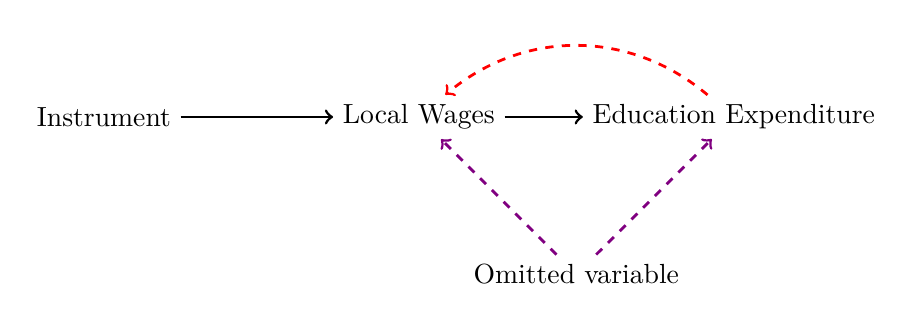
\begin{tikzpicture}
% nodes %
\node[rectangle] (z) at (0,0) {Instrument};
\node (t) at (4,0) {Local Wages};
\node (y) at (8,0) {Education Expenditure};
\node (u) at (6,-2) {Omitted variable};

% edges %
\draw[->, line width=1] (z) -- (t);
\draw[->, line width=1] (t) -- (y);
\draw[->, line width=1, violet, dashed] (u) -- (t);
\draw[->, line width=1, violet, dashed] (u) -- (y);
\draw[->, line width=1, red, bend right=40, dashed] (y) to (t);
\end{tikzpicture}
\label{fig:iv-approach}
\end{figure}

Shift-share or \emph{Bartik} instruments have gained popularity in
empirical work as a method of handling endogeneity issues in panel data
(Ferri (2022), Goldsmith-Pinkham, Sorkin, and Swift (2020), Bartik
(1991)). Such instruments combine time-variant, unit-invariant changes
in aggregate economic variables (ie., national changes in industry wage
levels) with time-invariant, unit-variant shares in exposure to these
macro-level changes (ie., local shares of employment in particular
industries). This decomposition of local-level changes via a
delocalisation over space and time allows for a defensible
`de-endogenising' of the treatment. Notably, the method can also be
considered to serve a further purpose as, by construction, it allows for
the examination of a macro phenomenon's effect on more local units.

\footnote{Autor et al. use a shift-share instrument to assess the effect
of Chinese import competition on manufacturing employment in US
commuting zones (@autor2013). As an extension, @feler2017 use a similar
shift-share instrument to assess the effect of the same shock on the
size of local government. @baccini2021 employ a shift-share instrument
for manufacturing layoffs to tease out the effect of a decline in
manufacturing on both economically motivated and racial identity voting
patterns in the US.}
\footnote{An additional popular indicator for modelling industrial shocks
is *oil price* as values are often assumed to be exogenous to local and
even national conditions (@scheer2022). Third, various indicators for measuring
*deindustrialisation* have been proposed including the manufacturing
share of employment, value added, and GDP [@tregenna2009,
@tregenna2020]. Finally, in rare instances,
exogeneity can be secured due to *geographical, climatological, or
geological factors*. For example, @borge2015 obtain an exogenous measure
of local revenue by "instrumenting the variation in hydropower revenue,
and thus total revenue, by topology, average precipitation and meters of
river in steep terrain." Certain authors have argued that the fact that
the location of hydrocarbon deposits is dictated by geomorphological
processes provides a plausible argument for exogeneity [@esposito2021,
@chen2022].}

Therefore, we adopt an identification strategy via a shift-share
instrument. A shift-share instrument interacts local industry shares
with national industry-level growth rates to obtain a plausibly
exogenous local shock. In the context of this work, we construct the
instrument by interacting a commuting-zone level constant industrial
employment share variable with national industry-level real value added
data.

The literature on Bartik instruments allows for an argument of plausible
exogeneity via various channels. First, authors argue that local
industry shares are exogenous by imposing that shares be fixed to a
particular base year and are therefore unable to adapt to changes in
national-level growth rates. Such a shift-share instrument would look as
follows:

\begin{equation}\phantomsection\label{eq-ref-bartik}{
Z_{it} = \sum_{j=1}^{k} S_{ij\tau}G_{njt}
}\end{equation}

where \(S_{ij\tau}\) is the local share of unit \(i\)'s economy
(measured using metrics like employment, wages, revenue) in industry
\(j\) at a fixed base year \(\tau\) and \(G_{njt}\) is the growth rate
of industry \(j\) at a national level \(n\) at time \(t\).

Alternatively, authors may argue that the claim of exogeneity in the
national-level growth rates is unlikely to be violated even when
allowing the local shares to vary over time. This approach is likely to
come at significant expense to instrument exogeneity. It is constructed
as follows:

\[
Z_{it} = \sum_{j=1}^{k} S_{ijt}G_{njt}
\]

Finally, authors might be concerned about the implausible exogeneity of
both shares and national-level growth rates in which case they could
construct the instrument as follows where the local shares are fixed at
a common base year and industry-specific growth rates \(G\) are derived
from data on other similar regions \(o\) rather than national-level
changes that are inherently comprised of local-level shifts. This
approach likely comes at significant expense to instrument relevance.

\[
Z_{it} = \sum_{j=1}^{k} S_{0jt}G_{ojt}
\]

Finally, the authors can make an additional design choice about whether
the effect of these instruments should be assumed common to an aggregate
local-level wage growth indicator or allowed to vary by industry. In
other words, whether to construct the first-stage relationship of the
2SLS as\ldots:

\[
X_{it} = \alpha_i + \beta\sum_{j=1}^{k}S_{ijt}G_{njt} + \epsilon_{it}
\]

\ldots or\ldots:

\[
X_{it} = \alpha_i + \sum_{j=1}^{k}\beta_{j}S_{j}G_{jt} + \epsilon_{it}
\]

We choose to employ the first of these options, assuming that industry
shares are only exogenous at a given base period and that national level
growth rates are exogenous and therefore allowed to vary with time.

Using data from the Bureau of Economic Analysis, we construct a
shift-share Bartik instruments at the commuting zone level using local
employment shares by industry and national changes in industry-specific
real value added represented in Equation~\ref{eq-bartik}. \(G_{njt}\)
represents national-level changes in value added in industry \(j\) in
time \(t\) and \(\frac{N_{ij\tau}}{N_{i\tau}}\) represents the
`sensitivity' of a CZ to these national shocks proxied by an initial
share of local employment in industry \(j\) in a baseline time period
\(\tau\). The product of these two values defines the shift-share
indicator \(\tilde{Z}_{i,t,s}\). In order to construct the share
portion, we compute the total local share of employment in a particular
industry \(j\). Due to challenges with missing data, we compute an
average share across 2001-2005 as our `base year'.

In the Appendices, we provide an additional estimation using a
wage-based shift-share instrument constructed using data from the US
Bureau of Labor Statistics' Quarterly Census of Employment and Wages
(QCEW). This shift-share instrument is constructed as described above
using industry-level changes in real wages. Concerns about endogeneity
are greater using this shift-share instrument and is therefore excluded
from the main text.

\footnote{We explore the sensitivity of results to the choice of base period
    $\tau$ by constructing the instrument for various base periods as
    well as a rolling window.}

\begin{equation}\phantomsection\label{eq-bartik}{
    \tilde{Z}_{it} = \sum_{j=1}^{k}G_{njt} *  \frac{N_{ij\tau}}{N_{i\tau}} 
}\end{equation}

This yields a 2SLS AR(1) model defined by the first- and second-stage
regressions represented in Equation~\ref{eq-first-stage} and
Equation~\ref{eq-second-stage}. Due to the likely presence of
time-dynamic effects, we include contemporaneous, 1-year, 2-year time
lags as instruments.

\begin{equation}\phantomsection\label{eq-first-stage}{
\textbf{(First stage)}\qquad
X_{it} \;=\; \phi\,X_{i,t-1} \;+\; \sum_{\ell=0}^{2}\pi_{\ell}\,\tilde Z_{i,t-\ell}
\;+\; \boldsymbol{\theta}\mathbf{W}_{it}' \;+\; \alpha_i \;+\; \lambda_t \;+\; u_{it},
}\end{equation}

\begin{equation}\phantomsection\label{eq-second-stage}{
\textbf{(Second stage)}\qquad
Y_{it} \;=\; \phi^\ast \,Y_{i,t-1} \;+\; \beta\,\widehat{X}_{it}
\;+\; \boldsymbol{\delta}\mathbf{W}_{it}'\;+\;  \alpha_i \;+\; \lambda_t \;+\; \varepsilon_{it}
}\end{equation}

where \(W_{it}\) is a vector of control variables. We control for
enrollment levels to account for scaling factors in education
expenditure, intergovernmental transfers to account for the significant
role of such transfers in funding education expenditure, percentage of
the population that is Black, percentage of the population that is
Hispanic, and private industry GDP per capita levels to account for
local price levels and economic performance.

\(Y_{it}\) is the natural logarithm of elementary (serving ages 6-12)
education expenditure per pupil for CZ \(i\) in year \(t\). We focus on
elementary education for two reasons. First, this restriction partly
shields against a justifiable concern about the endogeneity between
wages and quality of local public education. Whereas funding for high
school could likely affect local wages given such students are of
working age, funding for elementary education is unlikely to impact wage
rates via a human capital or skills channel. Second, in terms of public
impact, elementary education is of foundational importance in the lives
of children. Slips in public education provision at a young age could
have scarring effects.

\(\alpha_i\) represents a CZ fixed effect and \(\lambda_t\) represents
year-fixed effects, with stage-relevant superscripts.
\(\varepsilon_{it}\) and \(u_{it}\) represents the error term of the
second and first stage, respectively.

We compute the relevant shift-share instrument across 19 two-digit NAICS
industrial categories listed in \autoref{tbl_naics_codes}. Given
industry-level disaggregation of local employment data requires data
suppression for anonymity reasons, Figure 2 displays the data coverage
of our commuting zone level shift-share instruments. Given the high
degree of missingness in the 3-digit categorisation we proceed with the
2-digit NAICS codes in the rest of the work.

\begin{table}[ht]
\centering
\begin{tabular}{ll}
  \hline
NAICS.Code & Industry \\ 
  \hline
11 & Agriculture, Forestry, Fishing, and Hunting \\ 
  21 & Mining \\ 
  23 & Construction \\ 
  31-33 & Manufacturing \\ 
  42 & Wholesale Trade \\ 
  44-45 & Retail Trade \\ 
  48-49 & Transportation and Warehousing \\ 
  22 & Utilities \\ 
  51 & Information \\ 
  52 & Finance and Insurance \\ 
  53 & Real Estate and Rental and Leasing \\ 
  54 & Professional, Scientific, and Technical Services \\ 
  55 & Management of Companies and Enterprises \\ 
  56 & Administrative and waste management services \\ 
  61 & Educational Services \\ 
  62 & Health Care and Social Assistance \\ 
  71 & Arts, Entertainment, and Recreation \\ 
  72 & Accommodation and Food Services \\ 
  81 & Other Services, except government \\ 
  92 & Public Administration \\ 
   \hline
\end{tabular}
\caption{Industry Categories} 
\label{tbl_naics_codes}
\end{table}

\begin{figure}[H]

{\centering \pandocbounded{\includegraphics[keepaspectratio]{regressions_files/figure-pdf/fig_wage_elasticity-1.png}}

}

\caption{Data Coverage of Industry-level Employment as Share of Total
Reported Employed}

\end{figure}%

In \autoref{tbl_va_ss_baseline}, we demonstrate a strong and highly
significant first-stage relationship wherein our VA-based shift-share
instrument indicates a strong positive contemporaneous relationship with
local wages. We find that a 1\% increase in our shift-share instrument
raises local wages by 0.25\% in the same year though these wages rebound
as evidenced by the statistically significant negative coefficient of a
similar magnitude on the l1 regressor. Essentially, the time dynamics
indicate that local wages respond quickly to national sectoral shocks,
though not permanently. This can likely be interpreted as a temporary
local demand boom following industry-level value added shocks. This
provides additional evidence that the shift-share instrument captures
short-term exogenous variation rather than slow-moving trends in local
wages, boosting credibility in our instrumental variable relevance. The
growth rate specification in columns 3-4 provide further evidence of the
transitory nature of these demand shocks as only the contemporaneous
growth rate effect is significant.

The first-stage F-statistic using the level SS instrument is well above
conventional weak instrument thresholds confirming instrument relevance.
Furthermore, the Wu-Hausman tests reject the null of exogeneity,
confirming that OLS estimates are biased and IV estimation is
appropriate. Wald tests of joint significance further support the
strength of the instruments and the importance of incorporating
time-lagged instruments.

Using wage shocks in levels yields strong instruments, defensible
first-stage F-statistics, and stable second-stage estimates: positive
(negative) local wage shocks robustly decrease (increase) education
spending.

Taken together, these two specifications yield consistent and meaningful
results wherein the shift-share instrument allows for the causal
identification of negative relationship between local wage shocks and
education expenditure. The similarity in magnitude of the two designs
implies that the estimated effect is robust to the timing and
persistence of the underlying economic shocks. Most importantly, this
indicates that the mechanism identified is driven by temporary demand
shocks rather than permanent income effects. Interpretation of these
results requires a further exploration of local heterogeneity, outlined
in the following sections.

One could interpret this result as either a confirmation of resource
course dynamics in communities dependent on industries employing
lower-skill workers. If these effects are concentrated in less
economically prosperous areas, local wage booms in particular sectors
might be distracting public and administrative attention away from local
public education investments. On the other hand, if these effects are
driven by wage booms in communities reliant on higher-skill labour, one
could see this as a potential feedback between decreases in
intergovernmental revenues which are intended to be needs-based, even
though the specification controls for this effect, or potentially a
crowding out of public education by private education. The results below
do not provide a meaningful ability to distinguish the relative accuracy
of either of these hypotheses.

Computing bootstrap standard errors ( 399 replications)\ldots{} Using 8
cores for parallel bootstrap\ldots{} Bootstrap completed in 5.1 seconds

=== Standard Error Comparison === Variable Naive\_SE Bootstrap\_SE Ratio
l1\_log\_real\_Elem\_Educ\_Total\_Exp\_pp
l1\_log\_real\_Elem\_Educ\_Total\_Exp\_pp 0.0157 0.0152 0.9669
fitted\_endog log\_weighted\_annual\_avg\_wkly\_wage 0.0485 0.0502
1.0364 log\_real\_Total\_IG\_Revenue\_pp
log\_real\_Total\_IG\_Revenue\_pp 0.0210 0.0207 0.9889
log\_real\_gdp\_priv\_ind\_pc log\_real\_gdp\_priv\_ind\_pc 0.0144
0.0151 1.0519 log\_Enrollment log\_Enrollment 0.0158 0.0165 1.0440
pct\_black pct\_black 0.1886 0.1976 1.0477 pct\_hispanic pct\_hispanic
0.1509 0.1472 0.9756

Note: Ratio \textgreater{} 1 indicates naive SEs understate uncertainty

Computing bootstrap standard errors ( 399 replications)\ldots{} Using 8
cores for parallel bootstrap\ldots{} Bootstrap completed in 4.5 seconds

=== Standard Error Comparison === Variable Naive\_SE Bootstrap\_SE Ratio
fitted\_endog gr\_weighted\_annual\_avg\_wkly\_wage 0.7887 1.0888 1.3806
diff\_log\_real\_Total\_IG\_Revenue\_pp
diff\_log\_real\_Total\_IG\_Revenue\_pp 0.0317 0.0329 1.0358
diff\_log\_real\_gdp\_priv\_ind\_pc diff\_log\_real\_gdp\_priv\_ind\_pc
0.0473 0.0651 1.3761 diff\_log\_Enrollment diff\_log\_Enrollment 0.0425
0.0455 1.0712 fd\_pct\_black fd\_pct\_black 1.4189 1.3520 0.9528
fd\_pct\_hispanic fd\_pct\_hispanic 0.8236 0.9837 1.1944

Note: Ratio \textgreater{} 1 indicates naive SEs understate uncertainty

Computing bootstrap standard errors ( 399 replications)\ldots{} Using 8
cores for parallel bootstrap\ldots{} Bootstrap completed in 4.6 seconds

=== Standard Error Comparison === Variable Naive\_SE Bootstrap\_SE Ratio
fitted\_endog gr\_weighted\_annual\_avg\_wkly\_wage 0.6608 0.8774 1.3277
diff\_log\_real\_Total\_IG\_Revenue\_pp
diff\_log\_real\_Total\_IG\_Revenue\_pp 0.0317 0.0310 0.9788
diff\_log\_real\_gdp\_priv\_ind\_pc diff\_log\_real\_gdp\_priv\_ind\_pc
0.0405 0.0545 1.3464 diff\_log\_Enrollment diff\_log\_Enrollment 0.0419
0.0439 1.0482 fd\_pct\_black fd\_pct\_black 1.3713 1.3753 1.0029
fd\_pct\_hispanic fd\_pct\_hispanic 0.8161 0.8908 1.0915

Note: Ratio \textgreater{} 1 indicates naive SEs understate uncertainty

Computing bootstrap standard errors ( 399 replications)\ldots{} Using 8
cores for parallel bootstrap\ldots{} Bootstrap completed in 4.8 seconds

=== Standard Error Comparison === Variable Naive\_SE Bootstrap\_SE Ratio
l1\_log\_real\_Elem\_Educ\_Total\_Exp\_pp
l1\_log\_real\_Elem\_Educ\_Total\_Exp\_pp 0.0155 0.0158 1.0187
fitted\_endog gr\_weighted\_annual\_avg\_wkly\_wage 0.8583 1.6462 1.9180
log\_real\_Total\_IG\_Revenue\_pp log\_real\_Total\_IG\_Revenue\_pp
0.0219 0.0245 1.1172 log\_real\_gdp\_priv\_ind\_pc
log\_real\_gdp\_priv\_ind\_pc 0.0142 0.0187 1.3164 log\_Enrollment
log\_Enrollment 0.0145 0.0190 1.3066 pct\_black pct\_black 0.2426 0.3722
1.5343 pct\_hispanic pct\_hispanic 0.1814 0.2676 1.4750

Note: Ratio \textgreater{} 1 indicates naive SEs understate uncertainty

Computing bootstrap standard errors ( 399 replications)\ldots{} Using 8
cores for parallel bootstrap\ldots{} Bootstrap completed in 4.9 seconds

=== Standard Error Comparison === Variable Naive\_SE Bootstrap\_SE Ratio
l1\_log\_real\_Elem\_Educ\_Total\_Exp\_pp
l1\_log\_real\_Elem\_Educ\_Total\_Exp\_pp 0.0157 0.0160 1.0202
fitted\_endog log\_weighted\_annual\_avg\_wkly\_wage 0.0485 0.0472
0.9745 log\_real\_Total\_IG\_Revenue\_pp
log\_real\_Total\_IG\_Revenue\_pp 0.0210 0.0215 1.0256
log\_real\_gdp\_priv\_ind\_pc log\_real\_gdp\_priv\_ind\_pc 0.0144
0.0151 1.0485 log\_Enrollment log\_Enrollment 0.0158 0.0158 1.0004
pct\_black pct\_black 0.1886 0.1868 0.9906 pct\_hispanic pct\_hispanic
0.1509 0.1514 1.0036

Note: Ratio \textgreater{} 1 indicates naive SEs understate uncertainty

\begin{table}[htbp]
   \caption{\label{tbl_va_ss_baseline} IV Estimation Using VA-based Shift-share instrument (l0, l1, l2) in Levels with CZ and year fixed effects and lags.}
   \centering
   \begin{adjustbox}{width = \textwidth, center}
      \begin{tabular}{lcccc}
         \tabularnewline \midrule \midrule
         Dependent Variables:             & (log) Annual Avg. Wkly. Wage & (log) Elem.Ed.Exp.pp   & (GR) Annual Avg. Wkly. Wage & (GR) Elem.Ed.Exp.pp\\  
         Model:                           & (1)                          & (2)                    & (3)                         & (4)\\  
         \midrule
         \emph{Variables}\\
         VA SS (Lvl)                      & -0.0203                      &                        &                             &   \\   
                                          & (0.0353)                     &                        &                             &   \\   
         VA SS (Lvl, l1)                  & -0.1831$^{***}$              &                        &                             &   \\   
                                          & (0.0448)                     &                        &                             &   \\   
         VA SS (Lvl, l2)                  & 0.1668$^{***}$               &                        &                             &   \\   
                                          & (0.0391)                     &                        &                             &   \\   
         (log) IG Revenue pp              & 0.0143$^{***}$               & 0.2229$^{***}$         &                             &   \\   
                                          & (0.0017)                     & (0.0210)               &                             &   \\   
         (log) Real GDP Priv. Industry pc & 0.0394$^{***}$               & 0.0662$^{***}$         &                             &   \\   
                                          & (0.0015)                     & (0.0144)               &                             &   \\   
         (log) Enrollment                 & 0.0099$^{***}$               & -0.1955$^{***}$        &                             &   \\   
                                          & (0.0028)                     & (0.0158)               &                             &   \\   
         \% Black                         & -0.1668$^{***}$              & 0.3328$^{*}$           &                             &   \\   
                                          & (0.0450)                     & (0.1886)               &                             &   \\   
         \% Hispanic                      & -0.0529$^{**}$               & 0.0484                 &                             &   \\   
                                          & (0.0218)                     & (0.1509)               &                             &   \\   
         (log, l1) Annual Avg. Wkly. Wage & 0.7848$^{***}$               &                        &                             &   \\   
                                          & (0.0051)                     &                        &                             &   \\   
         (l1, log) Elem.Ed.Exp.pp         &                              & 0.5095$^{***}$         &                             &   \\   
                                          &                              & (0.0157)               &                             &   \\   
         (log) Annual Avg. Wkly. Wage     &                              & 0.2263$^{***}$         &                             &   \\   
                                          &                              & (0.0485)               &                             &   \\   
         VA SS (GR)                       &                              &                        & -0.1675$^{***}$             &   \\   
                                          &                              &                        & (0.0369)                    &   \\   
         VA SS (GR,l1)                    &                              &                        & -0.2374$^{***}$             &   \\   
                                          &                              &                        & (0.0411)                    &   \\   
         VA SS (GR,l2)                    &                              &                        & 0.0064                      &   \\   
                                          &                              &                        & (0.0497)                    &   \\   
         (GR) IG Revenue pp               &                              &                        & 0.0041                      & 0.3100$^{***}$\\   
                                          &                              &                        & (0.0025)                    & (0.0317)\\   
         (GR) Real GDP Priv. Industry pc  &                              &                        & 0.0593$^{***}$              & 0.0749\\   
                                          &                              &                        & (0.0026)                    & (0.0473)\\   
         (GR) Enrollment                  &                              &                        & 0.0153$^{***}$              & -0.5813$^{***}$\\   
                                          &                              &                        & (0.0059)                    & (0.0425)\\   
         fd\_pct\_black                   &                              &                        & -0.7505$^{***}$             & -1.298\\   
                                          &                              &                        & (0.1707)                    & (1.419)\\   
         fd\_pct\_hispanic                &                              &                        & 0.3005$^{**}$               & 1.817$^{**}$\\   
                                          &                              &                        & (0.1350)                    & (0.8236)\\   
         (GR) Annual Avg. Wkly. Wage      &                              &                        &                             & -1.313$^{*}$\\   
                                          &                              &                        &                             & (0.7887)\\   
         \midrule
         \emph{Fixed-effects}\\
         unit                             & Yes                          & Yes                    & Yes                         & Yes\\  
         year                             & Yes                          & Yes                    & Yes                         & Yes\\  
         \midrule
         \emph{Fit statistics}\\
         Observations                     & 12,084                       & 12,084                 & 12,084                      & 12,084\\  
         R$^2$                            & 0.99247                      & 0.90636                & 0.29876                     & 0.26621\\  
         Within R$^2$                     & 0.77617                      & 0.51804                & 0.04945                     & 0.21901\\  
         First-stage F                    &                              & 9.2412                 &                             & 14.495\\  
         F p-value                        &                              & $4.22\times 10^{-6}$   &                             & $2.02\times 10^{-9}$\\   
         First-stage F (marginal)         &                              & 15.675                 &                             & 14.495\\  
         F (marg) p-value                 &                              & $3.59\times 10^{-10}$  &                             & $2.02\times 10^{-9}$\\   
         Wu-Hausman                       &                              & 0.46756                &                             & 0.09282\\  
         WH p-value                       &                              & 0.49411                &                             & 0.76062\\  
         Sargan                           &                              & 66.871                 &                             & 28.172\\  
         Sargan p-value                   &                              & $3.01\times 10^{-15}$  &                             & $7.63\times 10^{-7}$\\   
         \midrule \midrule
         \multicolumn{5}{l}{\emph{Signif. Codes: ***: 0.01, **: 0.05, *: 0.1}}\\
      \end{tabular}
   \end{adjustbox}
\end{table}
\begin{table}[htbp]
   \caption{\label{tbl_va_ss_baseline} IV Estimation Using VA-based Shift-share instrument (l0, l1, l2) in Levels with CZ and year fixed effects and lags.}
   \centering
   \begin{adjustbox}{width = \textwidth, center}
      \begin{tabular}{lcccccc}
         \tabularnewline \midrule \midrule
         Dependent Variables:                                      & (log) Annual Avg. Wkly. Wage & (log) Elem.Ed.Exp.pp     & (log) Annual Avg. Wkly. Wage & (log) Elem.Ed.Exp.pp   & (log) Annual Avg. Wkly. Wage & (log) Elem.Ed.Exp.pp\\  
                                                                   & (FS) Manual IV - Full AR     & (SS) Manual IV - Full AR & (FS) Full AR                 & (SS) Full AR           & (FS) No AR                   & (SS) No AR \\   
         Model:                                                    & (1)                          & (2)                      & (3)                          & (4)                    & (5)                          & (6)\\  
         \midrule
         \emph{Variables}\\
         VA SS (Lvl)                                               & -0.0203                      &                          & -0.0179                      &                        & 0.2092$^{**}$                &   \\   
                                                                   & (0.0353)                     &                          & (0.0484)                     &                        & (0.1026)                     &   \\   
         VA SS (Lvl, l1)                                           & -0.1831$^{***}$              &                          & -0.1808$^{***}$              &                        & -0.3220$^{***}$              &   \\   
                                                                   & (0.0448)                     &                          & (0.0592)                     &                        & (0.0629)                     &   \\   
         VA SS (Lvl, l2)                                           & 0.1668$^{***}$               &                          & 0.1614$^{***}$               &                        & -0.0190                      &   \\   
                                                                   & (0.0391)                     &                          & (0.0497)                     &                        & (0.1069)                     &   \\   
         (log) IG Revenue pp                                       & 0.0143$^{***}$               & 0.2229$^{***}$           & 0.0135$^{***}$               & 0.2230$^{***}$         & 0.0453$^{***}$               & 0.4550$^{***}$\\   
                                                                   & (0.0017)                     & (0.0210)                 & (0.0030)                     & (0.0211)               & (0.0101)                     & (0.0617)\\   
         (log) Real GDP Priv. Industry pc                          & 0.0394$^{***}$               & 0.0662$^{***}$           & 0.0390$^{***}$               & 0.0662$^{***}$         & 0.1568$^{***}$               & 0.5716$^{***}$\\   
                                                                   & (0.0015)                     & (0.0144)                 & (0.0044)                     & (0.0144)               & (0.0156)                     & (0.1975)\\   
         (log) Enrollment                                          & 0.0099$^{***}$               & -0.1955$^{***}$          & 0.0109$^{**}$                & -0.1957$^{***}$        & 0.0629$^{***}$               & -0.1502$^{*}$\\   
                                                                   & (0.0028)                     & (0.0158)                 & (0.0044)                     & (0.0157)               & (0.0159)                     & (0.0825)\\   
         \% Black                                                  & -0.1668$^{***}$              & 0.3328$^{*}$             & -0.1685$^{**}$               & 0.3333$^{*}$           & -0.1519                      & 0.0962\\   
                                                                   & (0.0450)                     & (0.1886)                 & (0.0724)                     & (0.1924)               & (0.2154)                     & (0.7547)\\   
         \% Hispanic                                               & -0.0529$^{**}$               & 0.0484                   & -0.0526                      & 0.0483                 & 0.2279$^{**}$                & 0.6591\\   
                                                                   & (0.0218)                     & (0.1509)                 & (0.0327)                     & (0.1509)               & (0.1020)                     & (0.4309)\\   
         (log, l1) Annual Avg. Wkly. Wage                          & 0.7848$^{***}$               &                          & 0.7828$^{***}$               &                        &                              &   \\   
                                                                   & (0.0051)                     &                          & (0.0120)                     &                        &                              &   \\   
         (l1, log) Elem.Ed.Exp.pp                                  &                              & 0.5095$^{***}$           & 0.0039                       & 0.5086$^{***}$         &                              &   \\   
                                                                   &                              & (0.0157)                 & (0.0041)                     & (0.0156)               &                              &   \\   
         (log) Annual Avg. Wkly. Wage                              &                              & 0.2263$^{***}$           &                              & 0.2269$^{***}$         &                              & -2.463$^{**}$\\   
                                                                   &                              & (0.0485)                 &                              & (0.0477)               &                              & (1.173)\\   
         \midrule
         \emph{Fixed-effects}\\
         unit                                                      & Yes                          & Yes                      & Yes                          & Yes                    & Yes                          & Yes\\  
         year                                                      & Yes                          & Yes                      & Yes                          & Yes                    & Yes                          & Yes\\  
         \midrule
         \emph{Fit statistics}\\
         Observations                                              & 12,084                       & 12,084                   & 12,084                       & 12,084                 & 12,084                       & 12,084\\  
         R$^2$                                                     & 0.99247                      & 0.90636                  & 0.99247                      & 0.90636                & 0.97691                      & 0.86098\\  
         Within R$^2$                                              & 0.77617                      & 0.51804                  & 0.77623                      & 0.51804                & 0.31396                      & 0.28448\\  
         First-stage F                                             &                              & 9.2412                   &                              &                        &                              & \\  
         F p-value                                                 &                              & $4.22\times 10^{-6}$     &                              &                        &                              & \\  
         Wu-Hausman                                                &                              &                          &                              & 44.905                 &                              & 65.587\\  
         Wu-Hausman, p-value                                       &                              &                          &                              & $2.17\times 10^{-11}$  &                              & $6.12\times 10^{-16}$\\   
         Wald (IV only)                                            &                              &                          & 1,345.2                      & 22.645                 & 9.4020                       & 4.4097\\  
         Wald (IV only), p-value                                   &                              &                          & $0\times 10^{-16}$           & $1.97\times 10^{-6}$   & $3.34\times 10^{-6}$         & 0.03576\\  
         F-test (1st stage)                                        &                              &                          & 5,972.4                      &                        & 16.548                       & \\  
         F-test (1st stage), (log) Annual Avg. Wkly. Wage          &                              &                          &                              & 5,972.4                &                              & 16.548\\  
         F-test (1st stage), p-value                               &                              &                          & $0\times 10^{-16}$           &                        & $9.99\times 10^{-11}$        & \\  
         F-test (1st stage), p-value, (log) Annual Avg. Wkly. Wage &                              &                          &                              & $0\times 10^{-16}$     &                              & $9.99\times 10^{-11}$\\   
         First-stage F (marginal)                                  &                              & 15.675                   &                              &                        &                              & \\  
         F (marg) p-value                                          &                              & $3.59\times 10^{-10}$    &                              &                        &                              & \\  
         Wu-Hausman                                                &                              & 0.46756                  &                              &                        &                              & \\  
         WH p-value                                                &                              & 0.49411                  &                              &                        &                              & \\  
         Sargan                                                    &                              & 66.871                   &                              &                        &                              & \\  
         Sargan p-value                                            &                              & $3.01\times 10^{-15}$    &                              &                        &                              & \\  
         \midrule \midrule
         \multicolumn{7}{l}{\emph{Signif. Codes: ***: 0.01, **: 0.05, *: 0.1}}\\
      \end{tabular}
   \end{adjustbox}
\end{table}
\begin{table}[htbp]
   \caption{\label{tbl_va_ss_baseline} IV Estimation Using VA-based Shift-share instrument (l0, l1, l2) in Levels with CZ and year fixed effects and lags.}
   \centering
   \begin{adjustbox}{width = \textwidth, center}
      \begin{tabular}{lcccccc}
         \tabularnewline \midrule \midrule
         Dependent Variables:                                      & (log) Annual Avg. Wkly. Wage & (log) Elem.Ed.Exp.pp   & (log) Annual Avg. Wkly. Wage & (log) Elem.Ed.Exp.pp   & (log) Annual Avg. Wkly. Wage & (log) Elem.Ed.Exp.pp\\  
                                                                   & (FS) SS AR                   & (SS) SS AR             & (FS) FS AR                   & (SS) FS AR             & (FS) Full AR                 & (SS) Full AR \\   
         Model:                                                    & (1)                          & (2)                    & (3)                          & (4)                    & (5)                          & (6)\\  
         \midrule
         \emph{Variables}\\
         VA SS (Lvl)                                               & 0.2417$^{**}$                &                        & -0.0203                      &                        & -0.0179                      &   \\   
                                                                   & (0.1006)                     &                        & (0.0485)                     &                        & (0.0484)                     &   \\   
         VA SS (Lvl, l1)                                           & -0.2749$^{***}$              &                        & -0.1831$^{***}$              &                        & -0.1808$^{***}$              &   \\   
                                                                   & (0.0625)                     &                        & (0.0600)                     &                        & (0.0592)                     &   \\   
         VA SS (Lvl, l2)                                           & -0.1061                      &                        & 0.1668$^{***}$               &                        & 0.1614$^{***}$               &   \\   
                                                                   & (0.1058)                     &                        & (0.0516)                     &                        & (0.0497)                     &   \\   
         (l1, log) Elem.Ed.Exp.pp                                  & 0.0676$^{***}$               & 0.6475$^{***}$         &                              &                        & 0.0039                       & 0.5086$^{***}$\\   
                                                                   & (0.0086)                     & (0.0590)               &                              &                        & (0.0041)                     & (0.0156)\\   
         (log) IG Revenue pp                                       & 0.0304$^{***}$               & 0.2840$^{***}$         & 0.0143$^{***}$               & 0.3213$^{***}$         & 0.0135$^{***}$               & 0.2230$^{***}$\\   
                                                                   & (0.0098)                     & (0.0331)               & (0.0028)                     & (0.0316)               & (0.0030)                     & (0.0211)\\   
         (log) Real GDP Priv. Industry pc                          & 0.1459$^{***}$               & 0.3718$^{***}$         & 0.0394$^{***}$               & 0.0946$^{***}$         & 0.0390$^{***}$               & 0.0662$^{***}$\\   
                                                                   & (0.0155)                     & (0.1230)               & (0.0044)                     & (0.0243)               & (0.0044)                     & (0.0144)\\   
         (log) Enrollment                                          & 0.0781$^{***}$               & -0.0404                & 0.0099$^{**}$                & -0.3306$^{***}$        & 0.0109$^{**}$                & -0.1957$^{***}$\\   
                                                                   & (0.0155)                     & (0.0684)               & (0.0042)                     & (0.0282)               & (0.0044)                     & (0.0157)\\   
         \% Black                                                  & -0.1828                      & -0.1207                & -0.1668$^{**}$               & 0.6541$^{*}$           & -0.1685$^{**}$               & 0.3333$^{*}$\\   
                                                                   & (0.2105)                     & (0.4893)               & (0.0720)                     & (0.3622)               & (0.0724)                     & (0.1924)\\   
         \% Hispanic                                               & 0.2216$^{**}$                & 0.4591$^{*}$           & -0.0529                      & 0.0381                 & -0.0526                      & 0.0483\\   
                                                                   & (0.1029)                     & (0.2667)               & (0.0326)                     & (0.2516)               & (0.0327)                     & (0.1509)\\   
         (log) Annual Avg. Wkly. Wage                              &                              & -1.851$^{**}$          &                              & 0.5618$^{***}$         &                              & 0.2269$^{***}$\\   
                                                                   &                              & (0.7749)               &                              & (0.0765)               &                              & (0.0477)\\   
         (log, l1) Annual Avg. Wkly. Wage                          &                              &                        & 0.7848$^{***}$               &                        & 0.7828$^{***}$               &   \\   
                                                                   &                              &                        & (0.0113)                     &                        & (0.0120)                     &   \\   
         \midrule
         \emph{Fixed-effects}\\
         unit                                                      & Yes                          & Yes                    & Yes                          & Yes                    & Yes                          & Yes\\  
         year                                                      & Yes                          & Yes                    & Yes                          & Yes                    & Yes                          & Yes\\  
         \midrule
         \emph{Fit statistics}\\
         Observations                                              & 12,084                       & 12,084                 & 12,084                       & 12,084                 & 12,084                       & 12,084\\  
         R$^2$                                                     & 0.97765                      & 0.90596                & 0.99247                      & 0.86539                & 0.99247                      & 0.90636\\  
         Within R$^2$                                              & 0.33602                      & 0.51597                & 0.77617                      & 0.30715                & 0.77623                      & 0.51804\\  
         Wu-Hausman                                                &                              & 53.013                 &                              & 138.75                 &                              & 44.905\\  
         Wu-Hausman, p-value                                       &                              & $3.53\times 10^{-13}$  &                              & $7.64\times 10^{-32}$  &                              & $2.17\times 10^{-11}$\\   
         Wald (IV only)                                            & 7.9497                       & 5.7063                 & 1,517.9                      & 53.948                 & 1,345.2                      & 22.645\\  
         Wald (IV only), p-value                                   & $2.72\times 10^{-5}$         & 0.01692                & $0\times 10^{-16}$           & $2.19\times 10^{-13}$  & $0\times 10^{-16}$           & $1.97\times 10^{-6}$\\   
         F-test (1st stage)                                        & 19.489                       &                        & 6,261.7                      &                        & 5,972.4                      & \\  
         F-test (1st stage), (log) Annual Avg. Wkly. Wage          &                              & 19.489                 &                              & 6,261.7                &                              & 5,972.4\\  
         F-test (1st stage), p-value                               & $1.34\times 10^{-12}$        &                        & $0\times 10^{-16}$           &                        & $0\times 10^{-16}$           & \\  
         F-test (1st stage), p-value, (log) Annual Avg. Wkly. Wage &                              & $1.34\times 10^{-12}$  &                              & $0\times 10^{-16}$     &                              & $0\times 10^{-16}$\\   
         \midrule \midrule
         \multicolumn{7}{l}{\emph{Clustered (unit) standard-errors in parentheses}}\\
         \multicolumn{7}{l}{\emph{Signif. Codes: ***: 0.01, **: 0.05, *: 0.1}}\\
      \end{tabular}
   \end{adjustbox}
\end{table}

\FloatBarrier

\subsection{Accounting for
Heterogeneity}\label{accounting-for-heterogeneity}

In order to make meaningful policy-related insights, we need to unmask
the substantial heterogeneity obscured by the national-level average
treatment effects described above. These national-level estimates are
unlikely to apply uniformly across states and commuting zones.
Therefore, this next section is dedicated to unpacking this
heterogeneity. Below, we (1) explore various metrics of local economic
growth and decline to partition our sample in a data-driven manner,
employ (2) industry-by-industry and (2) state-by-state estimations in
our IV specifications using our VA-based shift-share instrument.

However, given the high degree of both structural (state-specific tax,
regulatory, and legislative regimes) and evolved heterogeneity
(industrial activity, income, inequality, economic diversity) the
proposed analysis necessitates a disaggregated estimation strategy to
truly account for the heterogeneity across the units of observation.
Therefore, subsequent treatment estimation is dedicated to
state-by-state, industry-by-industry, and a growth cohort sub-sampling
procedure taking into account legacy income and wage growth rates.

For completeness, we provide results of average treatment effects for
all implemented estimations in the Appendices.

\subsubsection{Declining vs.~Growing
Regions}\label{declining-vs.-growing-regions}

First, we identify declining and growing regions by estimating
commuting-zone wage and private industry GDP growth rates conditional on
state and national level growth rates and partition our sample across
this distribution.

In order to identify declining and growing commuting zones, we estimate
separate time series models by commuting zone as follows. These models
allow for the identification of commuting-zone level growth rates while
controlling for state and national trends in a two-step framework.
First, we orthogonalize the state-level growth rate with respect to the
national trend, isolating state-specific fluctuations unrelated to the
national business cycle:

\[
\widetilde{\Delta \log GDPpc}^{state}_{t} 
= \Delta \log GDPpc^{state}_{t} 
- \hat{\gamma}\, \Delta \log GDPpc^{nat}_{t}
\] Second, we regress commuting zone growth on both the national growth
rate and the orthogonalized state residuals, thereby decomposing local
growth into national, state, and idiosyncratic components. This approach
identifies commuting zones whose trajectories systematically diverge
from higher-level aggregate patterns, providing a clean measure of
relative local economic performance.

\[
\Delta \log GDPpc^{CZ}_{t} 
= \alpha_{g} 
+ \beta_{n} \, \Delta \log GDPpc^{nat}_{t} 
+ \beta_{s} \, \widetilde{\Delta \log GDPpc}^{state}_{t} 
+ \varepsilon_{t}
\]

In these equations, each GDP term represents the private industry GDP
per capita at the CZ, state, or national level, denoted by superscript.

\textcolor{red}{I think this can be supported by interesting literature from the "left behind" and "geographies of discontent" literature in which 'relative' economic performance is what matters most for individuals' happiness. Might be a conceptual leap but an interesting connection?}

Intuitively, this specification measures how much of each CZ's growth
can be explained by broader aggregate trends versus localized factors.
By controlling for orthogonalized state and national variation, the
estimated intercept (\(\alpha_{g}\)) and residual terms capture
persistent, region‐specific trends that are not driven by common
macroeconomic forces. This allows us to identify which commuting zones
are systematically growing or declining relative to their state and
national baselines, thereby providing a purer measure of local economic
dynamics that is robust to shared higher-level shocks.

We then classify commuting zones by the value of \(\alpha_{g}\) which
represents their deviation from state- and national-level GDP growth
rates. We estimate this trend deviation in per capita values of private
industry GDP.

\footnote{We provide similar analysis of gross GDP in the Appendix.}

Figure 3 plots the distribution of values of \(\alpha_g\) where the
vertical dashed lines represent the 25th and 75th percentiles.

Next, Figure 4 below demonstrates the considerable variability in
GDP-level growth rates across commuting zones in the US between
2001-2021. Visualising the per capita growth rate deviations by state
and region demonstrates heterogeneity in this variability across states
and regions. For example, Texas, Montana, and Colorado have outstanding
positive outliers in the distribution whereas Kentucky, Louisiana, South
Dakota have outstanding negative outliers.

Finally, Figure 5 represents the distribution of the loadings on the
residualised state factors and the national growth rates at the
commuting zone level.

We perform the same trend deviation calculation for wages where each
wage variable represents the commuting zone, state, and national level
growth rate in the weekly average wage as reported in QCEW.

\[
\widetilde{\Delta \log Wage}^{state}_{t} 
= \Delta \log Wage^{state}_{t} 
- \hat{\gamma}\, \Delta \log Wage^{nat}_{t}
\]

\[
\Delta \log Wage^{CZ}_{t} 
= \alpha_{w} 
+ \beta_{n} \, \Delta \log Wage^{nat}_{t} 
+ \beta_{s} \, \widetilde{\Delta \log Wage}^{state}_{t} 
+ \varepsilon_{t}
\]

In Figure 7, we see that there is similar variability though the
patterns do not consistently indicate the same high- and low-performing
outliers across states indicating that GDP and wage growth are not
consistently correlated across regions. We demonstrate this fact in
Figure 8 where, although there is a positive correlation between
commuting zone GDPpc and wage trend deviations, the decile-decile plot
demonstrates a noisy relationship largely driven by certain outliers.

Figure 11 presents a correlation coefficient by commuting zone between
the two rates, providing greater detail on this relationship.

\autoref{fig:wage-trends-plots-1} \autoref{fig:wage-trends-plots2}
\autoref{fig:wage-trends-plots3} \autoref{fig:wage-trends-plots4}
\autoref{fig:wage-trends-plots5} \ref{fig:wage-trends-plots}
\autoref{fig:wage-trends-plots}

\begin{figure}[H]

{\centering \pandocbounded{\includegraphics[keepaspectratio]{regressions_files/figure-pdf/wage_gdp_trend-1.png}}

}

\caption{GDPpc and Wage Growth Rates and Loadings}

\end{figure}%

\begin{figure}[H]

{\centering \pandocbounded{\includegraphics[keepaspectratio]{regressions_files/figure-pdf/wage_gdp_trend-2.png}}

}

\caption{Lollipop Plot of Wage and GDPpc Growth Rates}

\end{figure}%

Below, we display, by state, the Pearson correlation coefficient between
CZ level GDP growth rates and wage growth rates. Interestingly, many
states see nearly exclusively positive correlation coefficients, whereas
others see a mix of commuting zones where the relationship is positive
or negative.

\begin{figure}[H]

{\centering \pandocbounded{\includegraphics[keepaspectratio]{regressions_files/figure-pdf/unnamed-chunk-19-1.png}}

}

\caption{Correlation Between GDP Growth Rates and Wage Growth Rates by
State}

\end{figure}%

\paragraph{Sample Partitioning by Growth
Rates}\label{sample-partitioning-by-growth-rates}

Using these growth rates, we partition the sample according to the
percentiles described above. \autoref{tbl_gdp_ss_wage_subsamples} and
\autoref{tbl_gdp_ss_gdp_subsamples} examine how the relationship between
local economic conditions and elementary education expenditure per pupil
varies across structurally growing and declining regions as defined in
the previous section. We partition our sample into four sub-samples by
their values of \(\alpha_{w}\) and \(\alpha_{g}\) as shown in
Table~\ref{tbl-categories}.

\begin{longtable}[]{@{}ll@{}}
\caption{Category Definitions}\label{tbl-categories}\tabularnewline
\toprule\noalign{}
Category & Definition (\(\alpha_{w}\), \(\alpha_{g}\)) \\
\midrule\noalign{}
\endfirsthead
\toprule\noalign{}
Category & Definition (\(\alpha_{w}\), \(\alpha_{g}\)) \\
\midrule\noalign{}
\endhead
\bottomrule\noalign{}
\endlastfoot
Declining & \(\alpha < 0\) \\
Hyper-Declining & \(\alpha < P_{25}\) \\
Growing & \(\alpha > 0\) \\
Hyper-Growing & \(\alpha > P_{75}\) \\
\end{longtable}

Zones with negative (positive) values of \(\alpha_{w}\) or \(\alpha_g\)
are designated as declining (growing), while those in the bottom (P25)
and top (P75) quartiles are labelled hyper-declining and hyper-growing,
respectively. This stratification enables comparison of fiscal
responsiveness across local economies with different long-run growth
trajectories.

\autoref{tbl_gdp_ss_wage_subsamples} partitions CZs by \(\alpha_w\).
Interestingly, we see that the effect of intergovernmental revenue is
nearly half the size in hyper-growing areas than the hyper-declining
areas indicating the importance of intergovernmental transfers in areas
where wages are declining. Additionally, the scaling effects of
enrollment are only significant in regions where wages exhibit high
growth or are moderately declining. Furthermore, the role of private
industry GDP in local elementary education expenditure explains
variation in education expenditure in those regions in which scaling
laws do not seem to apply. Most importantly though, the negative
relationship between annual wages and elementary education expenditure
is only present in areas that exhibit historically hyper-declining or
moderately growing wage trends. Additionally, the first-stage F
statistics only support causal identification in these columns.

In regions where wages are already declining, positive wage shocks
decrease spending on local public education providing potential support
for a story in which regions with declining wages de-prioritise
education when positive wage shocks ``come to town.'' In the case of
moderately growing regions,

\autoref{tbl_gdp_ss_gdp_subsamples} partitions CZs by long-run GDP per
capita trends. When partitioning the sample by GDP growth rates, the
interpretation is more straight-forward. Areas in which GDP is
exhibiting relative decline, the causal relationship between wages and
education expenditure is consistent with high first stage F statistics,
convincing performance on the Wu-Hausman endogeneity test, and
defensible, albeit weak, performance on the Wald test. These results
suggest an asymmetric fiscal response where wage shocks in areas whose
GDP is declining, have a negative effect on local public education
spending, in contrast to growing regions.

\FloatBarrier

\begin{verbatim}

Computing bootstrap standard errors ( 399  replications)...
Using 8 cores for parallel bootstrap...
Bootstrap completed in 6.5 seconds

=== Standard Error Comparison ===
                                                             Variable Naive_SE Bootstrap_SE  Ratio
l1_log_real_Elem_Educ_Total_Exp_pp l1_log_real_Elem_Educ_Total_Exp_pp   0.0157       0.0158 1.0069
fitted_endog                        log_weighted_annual_avg_wkly_wage   0.0485       0.0477 0.9845
log_real_Total_IG_Revenue_pp             log_real_Total_IG_Revenue_pp   0.0210       0.0220 1.0472
log_real_gdp_priv_ind_pc                     log_real_gdp_priv_ind_pc   0.0144       0.0143 0.9930
log_Enrollment                                         log_Enrollment   0.0158       0.0159 1.0082
pct_black                                                   pct_black   0.1886       0.1990 1.0555
pct_hispanic                                             pct_hispanic   0.1509       0.1535 1.0175

Note: Ratio > 1 indicates naive SEs understate uncertainty

Computing bootstrap standard errors ( 399  replications)...
Using 8 cores for parallel bootstrap...
Bootstrap completed in 1.8 seconds

=== Standard Error Comparison ===
                                                             Variable Naive_SE Bootstrap_SE  Ratio
l1_log_real_Elem_Educ_Total_Exp_pp l1_log_real_Elem_Educ_Total_Exp_pp   0.0207       0.0207 1.0022
fitted_endog                        log_weighted_annual_avg_wkly_wage   0.0732       0.0741 1.0122
log_real_Total_IG_Revenue_pp             log_real_Total_IG_Revenue_pp   0.0398       0.0392 0.9847
log_real_gdp_priv_ind_pc                     log_real_gdp_priv_ind_pc   0.0346       0.0376 1.0885
log_Enrollment                                         log_Enrollment   0.0324       0.0332 1.0243
pct_black                                                   pct_black   0.2205       0.2711 1.2297
pct_hispanic                                             pct_hispanic   0.2248       0.2329 1.0357

Note: Ratio > 1 indicates naive SEs understate uncertainty

Computing bootstrap standard errors ( 399  replications)...
Using 8 cores for parallel bootstrap...
Bootstrap completed in 2.4 seconds

=== Standard Error Comparison ===
                                                             Variable Naive_SE Bootstrap_SE  Ratio
l1_log_real_Elem_Educ_Total_Exp_pp l1_log_real_Elem_Educ_Total_Exp_pp   0.0190       0.0204 1.0696
fitted_endog                        log_weighted_annual_avg_wkly_wage   0.0639       0.0687 1.0740
log_real_Total_IG_Revenue_pp             log_real_Total_IG_Revenue_pp   0.0340       0.0331 0.9718
log_real_gdp_priv_ind_pc                     log_real_gdp_priv_ind_pc   0.0309       0.0317 1.0246
log_Enrollment                                         log_Enrollment   0.0234       0.0245 1.0475
pct_black                                                   pct_black   0.1957       0.2056 1.0506
pct_hispanic                                             pct_hispanic   0.1690       0.1701 1.0064

Note: Ratio > 1 indicates naive SEs understate uncertainty

Computing bootstrap standard errors ( 399  replications)...
Using 8 cores for parallel bootstrap...
Bootstrap completed in 3.1 seconds

=== Standard Error Comparison ===
                                                             Variable Naive_SE Bootstrap_SE  Ratio
l1_log_real_Elem_Educ_Total_Exp_pp l1_log_real_Elem_Educ_Total_Exp_pp   0.0219       0.0215 0.9812
fitted_endog                        log_weighted_annual_avg_wkly_wage   0.0602       0.0624 1.0368
log_real_Total_IG_Revenue_pp             log_real_Total_IG_Revenue_pp   0.0273       0.0269 0.9859
log_real_gdp_priv_ind_pc                     log_real_gdp_priv_ind_pc   0.0162       0.0162 1.0028
log_Enrollment                                         log_Enrollment   0.0211       0.0224 1.0585
pct_black                                                   pct_black   0.3369       0.3472 1.0307
pct_hispanic                                             pct_hispanic   0.1945       0.1893 0.9733

Note: Ratio > 1 indicates naive SEs understate uncertainty

Computing bootstrap standard errors ( 399  replications)...
Using 8 cores for parallel bootstrap...
Bootstrap completed in 1.8 seconds

=== Standard Error Comparison ===
                                                             Variable Naive_SE Bootstrap_SE  Ratio
l1_log_real_Elem_Educ_Total_Exp_pp l1_log_real_Elem_Educ_Total_Exp_pp   0.0282       0.0276 0.9799
fitted_endog                        log_weighted_annual_avg_wkly_wage   0.0804       0.0826 1.0282
log_real_Total_IG_Revenue_pp             log_real_Total_IG_Revenue_pp   0.0394       0.0389 0.9863
log_real_gdp_priv_ind_pc                     log_real_gdp_priv_ind_pc   0.0173       0.0189 1.0931
log_Enrollment                                         log_Enrollment   0.0296       0.0315 1.0660
pct_black                                                   pct_black   0.7404       0.7926 1.0705
pct_hispanic                                             pct_hispanic   0.2183       0.2299 1.0531

Note: Ratio > 1 indicates naive SEs understate uncertainty
\end{verbatim}

\begin{verbatim}

Computing bootstrap standard errors ( 399  replications)...
Using 8 cores for parallel bootstrap...
Bootstrap completed in 5.4 seconds

=== Standard Error Comparison ===
                                                             Variable Naive_SE Bootstrap_SE  Ratio
l1_log_real_Elem_Educ_Total_Exp_pp l1_log_real_Elem_Educ_Total_Exp_pp   0.0157       0.0152 0.9677
fitted_endog                        log_weighted_annual_avg_wkly_wage   0.0485       0.0487 1.0037
log_real_Total_IG_Revenue_pp             log_real_Total_IG_Revenue_pp   0.0210       0.0205 0.9772
log_real_gdp_priv_ind_pc                     log_real_gdp_priv_ind_pc   0.0144       0.0152 1.0598
log_Enrollment                                         log_Enrollment   0.0158       0.0154 0.9768
pct_black                                                   pct_black   0.1886       0.1966 1.0424
pct_hispanic                                             pct_hispanic   0.1509       0.1495 0.9909

Note: Ratio > 1 indicates naive SEs understate uncertainty

Computing bootstrap standard errors ( 399  replications)...
Using 8 cores for parallel bootstrap...
Bootstrap completed in 1.8 seconds

=== Standard Error Comparison ===
                                                             Variable Naive_SE Bootstrap_SE  Ratio
l1_log_real_Elem_Educ_Total_Exp_pp l1_log_real_Elem_Educ_Total_Exp_pp   0.0266       0.0260 0.9759
fitted_endog                        log_weighted_annual_avg_wkly_wage   0.0683       0.0732 1.0717
log_real_Total_IG_Revenue_pp             log_real_Total_IG_Revenue_pp   0.0336       0.0320 0.9531
log_real_gdp_priv_ind_pc                     log_real_gdp_priv_ind_pc   0.0234       0.0245 1.0472
log_Enrollment                                         log_Enrollment   0.0250       0.0274 1.0966
pct_black                                                   pct_black   0.2594       0.3185 1.2279
pct_hispanic                                             pct_hispanic   0.2536       0.2545 1.0036

Note: Ratio > 1 indicates naive SEs understate uncertainty

Computing bootstrap standard errors ( 399  replications)...
Using 8 cores for parallel bootstrap...
Bootstrap completed in 1.4 seconds

=== Standard Error Comparison ===
                                                             Variable Naive_SE Bootstrap_SE  Ratio
l1_log_real_Elem_Educ_Total_Exp_pp l1_log_real_Elem_Educ_Total_Exp_pp   0.0332       0.0343 1.0335
fitted_endog                        log_weighted_annual_avg_wkly_wage   0.0851       0.0910 1.0700
log_real_Total_IG_Revenue_pp             log_real_Total_IG_Revenue_pp   0.0313       0.0335 1.0712
log_real_gdp_priv_ind_pc                     log_real_gdp_priv_ind_pc   0.0304       0.0330 1.0843
log_Enrollment                                         log_Enrollment   0.0343       0.0386 1.1258
pct_black                                                   pct_black   0.3559       0.4815 1.3529
pct_hispanic                                             pct_hispanic   0.1887       0.2108 1.1170

Note: Ratio > 1 indicates naive SEs understate uncertainty

Computing bootstrap standard errors ( 399  replications)...
Using 8 cores for parallel bootstrap...
Bootstrap completed in 4.8 seconds

=== Standard Error Comparison ===
                                                             Variable Naive_SE Bootstrap_SE  Ratio
l1_log_real_Elem_Educ_Total_Exp_pp l1_log_real_Elem_Educ_Total_Exp_pp   0.0173       0.0166 0.9589
fitted_endog                        log_weighted_annual_avg_wkly_wage   0.0535       0.0478 0.8929
log_real_Total_IG_Revenue_pp             log_real_Total_IG_Revenue_pp   0.0238       0.0247 1.0397
log_real_gdp_priv_ind_pc                     log_real_gdp_priv_ind_pc   0.0151       0.0152 1.0080
log_Enrollment                                         log_Enrollment   0.0176       0.0172 0.9782
pct_black                                                   pct_black   0.2254       0.2534 1.1243
pct_hispanic                                             pct_hispanic   0.1782       0.1823 1.0229

Note: Ratio > 1 indicates naive SEs understate uncertainty

Computing bootstrap standard errors ( 399  replications)...
Using 8 cores for parallel bootstrap...
Bootstrap completed in 1.8 seconds

=== Standard Error Comparison ===
                                                             Variable Naive_SE Bootstrap_SE  Ratio
l1_log_real_Elem_Educ_Total_Exp_pp l1_log_real_Elem_Educ_Total_Exp_pp   0.0293       0.0298 1.0180
fitted_endog                        log_weighted_annual_avg_wkly_wage   0.0834       0.0886 1.0615
log_real_Total_IG_Revenue_pp             log_real_Total_IG_Revenue_pp   0.0388       0.0403 1.0381
log_real_gdp_priv_ind_pc                     log_real_gdp_priv_ind_pc   0.0162       0.0160 0.9828
log_Enrollment                                         log_Enrollment   0.0335       0.0349 1.0444
pct_black                                                   pct_black   0.5381       0.5339 0.9921
pct_hispanic                                             pct_hispanic   0.3026       0.3125 1.0327

Note: Ratio > 1 indicates naive SEs understate uncertainty
\end{verbatim}

\FloatBarrier

\begin{verbatim}

Computing bootstrap standard errors ( 399  replications)...
Using 8 cores for parallel bootstrap...
Bootstrap completed in 4.9 seconds

=== Standard Error Comparison ===
                                                             Variable Naive_SE Bootstrap_SE  Ratio
l1_log_real_Elem_Educ_Total_Exp_pp l1_log_real_Elem_Educ_Total_Exp_pp   0.0157       0.0164 1.0447
fitted_endog                        log_weighted_annual_avg_wkly_wage   0.0485       0.0505 1.0407
log_real_Total_IG_Revenue_pp             log_real_Total_IG_Revenue_pp   0.0210       0.0217 1.0364
log_real_gdp_priv_ind_pc                     log_real_gdp_priv_ind_pc   0.0144       0.0147 1.0201
log_Enrollment                                         log_Enrollment   0.0158       0.0164 1.0370
pct_black                                                   pct_black   0.1886       0.2085 1.1059
pct_hispanic                                             pct_hispanic   0.1509       0.1433 0.9495

Note: Ratio > 1 indicates naive SEs understate uncertainty

Computing bootstrap standard errors ( 399  replications)...
Using 8 cores for parallel bootstrap...
Bootstrap completed in 1.4 seconds

=== Standard Error Comparison ===
                                                             Variable Naive_SE Bootstrap_SE  Ratio
l1_log_real_Elem_Educ_Total_Exp_pp l1_log_real_Elem_Educ_Total_Exp_pp   0.0207       0.0213 1.0291
fitted_endog                        log_weighted_annual_avg_wkly_wage   0.0732       0.0796 1.0873
log_real_Total_IG_Revenue_pp             log_real_Total_IG_Revenue_pp   0.0398       0.0421 1.0584
log_real_gdp_priv_ind_pc                     log_real_gdp_priv_ind_pc   0.0346       0.0365 1.0549
log_Enrollment                                         log_Enrollment   0.0324       0.0342 1.0558
pct_black                                                   pct_black   0.2205       0.2533 1.1492
pct_hispanic                                             pct_hispanic   0.2248       0.2232 0.9928

Note: Ratio > 1 indicates naive SEs understate uncertainty

Computing bootstrap standard errors ( 399  replications)...
Using 8 cores for parallel bootstrap...
Bootstrap completed in 2.1 seconds

=== Standard Error Comparison ===
                                                             Variable Naive_SE Bootstrap_SE  Ratio
l1_log_real_Elem_Educ_Total_Exp_pp l1_log_real_Elem_Educ_Total_Exp_pp   0.0190       0.0183 0.9609
fitted_endog                        log_weighted_annual_avg_wkly_wage   0.0639       0.0638 0.9985
log_real_Total_IG_Revenue_pp             log_real_Total_IG_Revenue_pp   0.0340       0.0331 0.9713
log_real_gdp_priv_ind_pc                     log_real_gdp_priv_ind_pc   0.0309       0.0318 1.0288
log_Enrollment                                         log_Enrollment   0.0234       0.0223 0.9523
pct_black                                                   pct_black   0.1957       0.2155 1.1009
pct_hispanic                                             pct_hispanic   0.1690       0.1674 0.9903

Note: Ratio > 1 indicates naive SEs understate uncertainty

Computing bootstrap standard errors ( 399  replications)...
Using 8 cores for parallel bootstrap...
Bootstrap completed in 2.8 seconds

=== Standard Error Comparison ===
                                                             Variable Naive_SE Bootstrap_SE  Ratio
l1_log_real_Elem_Educ_Total_Exp_pp l1_log_real_Elem_Educ_Total_Exp_pp   0.0219       0.0242 1.1039
fitted_endog                        log_weighted_annual_avg_wkly_wage   0.0602       0.0635 1.0555
log_real_Total_IG_Revenue_pp             log_real_Total_IG_Revenue_pp   0.0273       0.0289 1.0592
log_real_gdp_priv_ind_pc                     log_real_gdp_priv_ind_pc   0.0162       0.0164 1.0107
log_Enrollment                                         log_Enrollment   0.0211       0.0220 1.0395
pct_black                                                   pct_black   0.3369       0.3550 1.0538
pct_hispanic                                             pct_hispanic   0.1945       0.1896 0.9748

Note: Ratio > 1 indicates naive SEs understate uncertainty

Computing bootstrap standard errors ( 399  replications)...
Using 8 cores for parallel bootstrap...
Bootstrap completed in 1.5 seconds

=== Standard Error Comparison ===
                                                             Variable Naive_SE Bootstrap_SE  Ratio
l1_log_real_Elem_Educ_Total_Exp_pp l1_log_real_Elem_Educ_Total_Exp_pp   0.0282       0.0283 1.0037
fitted_endog                        log_weighted_annual_avg_wkly_wage   0.0804       0.0863 1.0738
log_real_Total_IG_Revenue_pp             log_real_Total_IG_Revenue_pp   0.0394       0.0412 1.0458
log_real_gdp_priv_ind_pc                     log_real_gdp_priv_ind_pc   0.0173       0.0180 1.0380
log_Enrollment                                         log_Enrollment   0.0296       0.0301 1.0180
pct_black                                                   pct_black   0.7404       0.8096 1.0934
pct_hispanic                                             pct_hispanic   0.2183       0.2279 1.0442

Note: Ratio > 1 indicates naive SEs understate uncertainty
\end{verbatim}

\begin{verbatim}

Computing bootstrap standard errors ( 399  replications)...
Using 8 cores for parallel bootstrap...
Bootstrap completed in 4.9 seconds

=== Standard Error Comparison ===
                                                             Variable Naive_SE Bootstrap_SE  Ratio
l1_log_real_Elem_Educ_Total_Exp_pp l1_log_real_Elem_Educ_Total_Exp_pp   0.0157       0.0157 0.9981
fitted_endog                        log_weighted_annual_avg_wkly_wage   0.0485       0.0479 0.9878
log_real_Total_IG_Revenue_pp             log_real_Total_IG_Revenue_pp   0.0210       0.0216 1.0306
log_real_gdp_priv_ind_pc                     log_real_gdp_priv_ind_pc   0.0144       0.0152 1.0574
log_Enrollment                                         log_Enrollment   0.0158       0.0157 0.9916
pct_black                                                   pct_black   0.1886       0.2078 1.1019
pct_hispanic                                             pct_hispanic   0.1509       0.1485 0.9845

Note: Ratio > 1 indicates naive SEs understate uncertainty

Computing bootstrap standard errors ( 399  replications)...
Using 8 cores for parallel bootstrap...
Bootstrap completed in 1.5 seconds

=== Standard Error Comparison ===
                                                             Variable Naive_SE Bootstrap_SE  Ratio
l1_log_real_Elem_Educ_Total_Exp_pp l1_log_real_Elem_Educ_Total_Exp_pp   0.0266       0.0269 1.0090
fitted_endog                        log_weighted_annual_avg_wkly_wage   0.0683       0.0692 1.0132
log_real_Total_IG_Revenue_pp             log_real_Total_IG_Revenue_pp   0.0336       0.0342 1.0197
log_real_gdp_priv_ind_pc                     log_real_gdp_priv_ind_pc   0.0234       0.0242 1.0376
log_Enrollment                                         log_Enrollment   0.0250       0.0250 0.9978
pct_black                                                   pct_black   0.2594       0.3117 1.2016
pct_hispanic                                             pct_hispanic   0.2536       0.2613 1.0308

Note: Ratio > 1 indicates naive SEs understate uncertainty

Computing bootstrap standard errors ( 399  replications)...
Using 8 cores for parallel bootstrap...
Bootstrap completed in 1 seconds

=== Standard Error Comparison ===
                                                             Variable Naive_SE Bootstrap_SE  Ratio
l1_log_real_Elem_Educ_Total_Exp_pp l1_log_real_Elem_Educ_Total_Exp_pp   0.0332       0.0361 1.0899
fitted_endog                        log_weighted_annual_avg_wkly_wage   0.0851       0.0896 1.0530
log_real_Total_IG_Revenue_pp             log_real_Total_IG_Revenue_pp   0.0313       0.0329 1.0522
log_real_gdp_priv_ind_pc                     log_real_gdp_priv_ind_pc   0.0304       0.0355 1.1657
log_Enrollment                                         log_Enrollment   0.0343       0.0365 1.0648
pct_black                                                   pct_black   0.3559       0.4287 1.2044
pct_hispanic                                             pct_hispanic   0.1887       0.2057 1.0901

Note: Ratio > 1 indicates naive SEs understate uncertainty

Computing bootstrap standard errors ( 399  replications)...
Using 8 cores for parallel bootstrap...
Bootstrap completed in 4.3 seconds

=== Standard Error Comparison ===
                                                             Variable Naive_SE Bootstrap_SE  Ratio
l1_log_real_Elem_Educ_Total_Exp_pp l1_log_real_Elem_Educ_Total_Exp_pp   0.0173       0.0170 0.9825
fitted_endog                        log_weighted_annual_avg_wkly_wage   0.0535       0.0526 0.9830
log_real_Total_IG_Revenue_pp             log_real_Total_IG_Revenue_pp   0.0238       0.0241 1.0138
log_real_gdp_priv_ind_pc                     log_real_gdp_priv_ind_pc   0.0151       0.0157 1.0408
log_Enrollment                                         log_Enrollment   0.0176       0.0174 0.9891
pct_black                                                   pct_black   0.2254       0.2354 1.0446
pct_hispanic                                             pct_hispanic   0.1782       0.1804 1.0120

Note: Ratio > 1 indicates naive SEs understate uncertainty

Computing bootstrap standard errors ( 399  replications)...
Using 8 cores for parallel bootstrap...
Bootstrap completed in 1.5 seconds

=== Standard Error Comparison ===
                                                             Variable Naive_SE Bootstrap_SE  Ratio
l1_log_real_Elem_Educ_Total_Exp_pp l1_log_real_Elem_Educ_Total_Exp_pp   0.0293       0.0298 1.0185
fitted_endog                        log_weighted_annual_avg_wkly_wage   0.0834       0.0868 1.0397
log_real_Total_IG_Revenue_pp             log_real_Total_IG_Revenue_pp   0.0388       0.0405 1.0428
log_real_gdp_priv_ind_pc                     log_real_gdp_priv_ind_pc   0.0162       0.0174 1.0702
log_Enrollment                                         log_Enrollment   0.0335       0.0341 1.0185
pct_black                                                   pct_black   0.5381       0.6185 1.1493
pct_hispanic                                             pct_hispanic   0.3026       0.3175 1.0491

Note: Ratio > 1 indicates naive SEs understate uncertainty
\end{verbatim}

\begin{verbatim}
                                              All   Hyper-Declining (W..     Declining (Wage)       Growing (Wage) Hyper-Growing (Wage)
                                              All Hyper-Declining (Wage)     Declining (Wage)       Growing (Wage) Hyper-Growing (Wage)
\end{verbatim}

Dependent Var.: (log) Elem.Ed.Exp.pp (log) Elem.Ed.Exp.pp (log)
Elem.Ed.Exp.pp (log) Elem.Ed.Exp.pp (log) Elem.Ed.Exp.pp

(l1, log) Elem.Ed.Exp.pp 0.5095*** 0.5132*** 0.5507*** 0.5030***
0.5319\textbf{\emph{ (0.0157) (0.0266) (0.0332) (0.0174) (0.0293)\\
fitted\_endog 0.2263}} 0.3288*** 0.3420*** 0.2122*** 0.1548\\
(0.0485) (0.0683) (0.0851) (0.0535) (0.0834)\\
(log) IG Revenue pp 0.2229*** 0.2803*** 0.2106*** 0.2243***
0.1552\textbf{\emph{ (0.0210) (0.0336) (0.0313) (0.0238) (0.0388)\\
(log) Real GDP Priv. Industry pc 0.0662}} 0.0156 0.0220 0.0703***
0.0685\textbf{\emph{ (0.0144) (0.0234) (0.0305) (0.0150) (0.0162)\\
(log) Enrollment -0.1955}} -0.2275*** -0.2009*** -0.1938***
-0.2000**\emph{ (0.0158) (0.0250) (0.0343) (0.0176) (0.0335)\\
\% Black 0.3328 0.2169 0.2131 0.3884 1.192}\\
(0.1886) (0.2594) (0.3559) (0.2254) (0.5381)\\
\% Hispanic 0.0484 0.2612 0.2542 0.0112 0.1339\\
(0.1509) (0.2536) (0.1887) (0.1782) (0.3026)\\
Fixed-Effects: -------------------- --------------------
-------------------- -------------------- -------------------- unit Yes
Yes Yes Yes Yes year Yes Yes Yes Yes Yes
\_\_\_\_\_\_\_\_\_\_\_\_\_\_\_\_\_\_\_\_\_\_\_\_\_\_\_\_\_\_\_\_
\_\_\_\_\_\_\_\_\_\_\_\_\_\_\_\_\_\_\_\_
\_\_\_\_\_\_\_\_\_\_\_\_\_\_\_\_\_\_\_\_
\_\_\_\_\_\_\_\_\_\_\_\_\_\_\_\_\_\_\_\_
\_\_\_\_\_\_\_\_\_\_\_\_\_\_\_\_\_\_\_\_
\_\_\_\_\_\_\_\_\_\_\_\_\_\_\_\_\_\_\_\_ S.E.: Clustered by: unit by:
unit by: unit by: unit by: unit Observations 12,084 3,021 1,520 10,564
3,021 R2 0.90636 0.92102 0.94210 0.89805 0.90098 Within R2 0.51804
0.57170 0.58940 0.50753 0.50064 First-stage F 9.2412 5.3600 6.4764
10.356 2.7055 F p-value 4.22e-6 0.00111 0.00024 8.41e-7 0.04386
First-stage F (marginal) 15.675 5.6257 5.5599 19.379 11.901 F (marg)
p-value 3.59e-10 0.00077 0.00086 1.59e-12 9.61e-8 Wu-Hausman 0.46756
0.06497 0.01588 0.58897 2.3350 WH p-value 0.49411 0.79880 0.89973
0.44282 0.12649 Sargan 66.871 42.439 34.534 38.772 11.434 Sargan p-value
3.01e-15 6.09e-10 3.17e-8 3.81e-9 0.00329 --- Signif. codes: 0
`\emph{\textbf{' 0.001 '}' 0.01 '}' 0.05 `.' 0.1 ' ' 1 All
Hyper-Declining (Wage) Declining (Wage) Growing (Wage) Hyper-Growing
(Wage) All Hyper-Declining (Wage) Declining (Wage) Growing (Wage)
Hyper-Growing (Wage) Dependent Var.: (log) Annual Avg. Wkly. Wage (log)
Annual Avg. Wkly. Wage (log) Annual Avg. Wkly. Wage (log) Annual Avg.
Wkly. Wage (log) Annual Avg. Wkly. Wage

VA SS (Lvl) -0.0203 -0.0218 0.1082 -0.0497 0.1516\\
(0.0353) (0.0529) (0.0716) (0.0410) (0.1059)\\
VA SS (Lvl, l1) -0.1831*** -0.1717* -0.3005*** -0.1466** -0.3541**
(0.0448) (0.0673) (0.0893) (0.0521) (0.1343)\\
VA SS (Lvl, l2) 0.1668*** 0.2313*** 0.2726*** 0.1188** 0.1489\\
(0.0391) (0.0602) (0.0826) (0.0446) (0.1119)\\
(log) IG Revenue pp 0.0143*** 0.0097** 0.0095* 0.0141***
0.0161\textbf{\emph{ (0.0017) (0.0034) (0.0047) (0.0018) (0.0038)\\
(log) Real GDP Priv. Industry pc 0.0394}} 0.0656*** 0.0633*** 0.0375***
0.0313\textbf{\emph{ (0.0015) (0.0042) (0.0056) (0.0016) (0.0026)\\
(log) Enrollment 0.0099}} 0.0175*** 0.0185** 0.0086** 0.0026\\
(0.0028) (0.0049) (0.0068) (0.0031) (0.0070)\\
\% Black -0.1668*** -0.1666** -0.2457** -0.1323** -0.1830\\
(0.0450) (0.0624) (0.0950) (0.0505) (0.1513)\\
\% Hispanic -0.0529* -0.0806* -0.0149 -0.0480* -0.0318\\
(0.0218) (0.0374) (0.0529) (0.0237) (0.0572)\\
(log, l1) Annual Avg. Wkly. Wage 0.7848*** 0.7824*** 0.8181*** 0.7784***
0.7634*** (0.0051) (0.0108) (0.0145) (0.0055) (0.0112)\\
Fixed-Effects: ---------------------------- ----------------------------
---------------------------- ----------------------------
---------------------------- unit Yes Yes Yes Yes Yes year Yes Yes Yes
Yes Yes \_\_\_\_\_\_\_\_\_\_\_\_\_\_\_\_\_\_\_\_\_\_\_\_\_\_\_\_\_\_\_\_
\_\_\_\_\_\_\_\_\_\_\_\_\_\_\_\_\_\_\_\_\_\_\_\_\_\_\_\_
\_\_\_\_\_\_\_\_\_\_\_\_\_\_\_\_\_\_\_\_\_\_\_\_\_\_\_\_
\_\_\_\_\_\_\_\_\_\_\_\_\_\_\_\_\_\_\_\_\_\_\_\_\_\_\_\_
\_\_\_\_\_\_\_\_\_\_\_\_\_\_\_\_\_\_\_\_\_\_\_\_\_\_\_\_
\_\_\_\_\_\_\_\_\_\_\_\_\_\_\_\_\_\_\_\_\_\_\_\_\_\_\_\_ S.E. type IID
IID IID IID IID Observations 12,084 3,021 1,520 10,564 3,021 R2 0.99247
0.99486 0.99528 0.99172 0.98787 Within R2 0.77617 0.74723 0.78987
0.77401 0.74615 --- Signif. codes: 0 `\emph{\textbf{' 0.001 '}' 0.01 '}'
0.05 `.' 0.1 ' ' 1 All Hyper-Declining (G.. Declining (GDP) Growing
(GDP) Hyper-Growing (GDP) All Hyper-Declining (GDP) Declining (GDP)
Growing (GDP) Hyper-Growing (GDP) Dependent Var.: (log) Elem.Ed.Exp.pp
(log) Elem.Ed.Exp.pp (log) Elem.Ed.Exp.pp (log) Elem.Ed.Exp.pp (log)
Elem.Ed.Exp.pp

(l1, log) Elem.Ed.Exp.pp 0.5095*** 0.5416*** 0.5280*** 0.4952***
0.4901\textbf{\emph{ (0.0157) (0.0207) (0.0190) (0.0219) (0.0282)\\
fitted\_endog 0.2263}} 0.2791*** 0.2915*** 0.1867** 0.2528** (0.0485)
(0.0732) (0.0639) (0.0602) (0.0804)\\
(log) IG Revenue pp 0.2229*** 0.2292*** 0.2576*** 0.2083***
0.1910\textbf{\emph{ (0.0210) (0.0398) (0.0340) (0.0273) (0.0394)\\
(log) Real GDP Priv. Industry pc 0.0662}} 0.0378 0.0398 0.0713***
0.0758\textbf{\emph{ (0.0144) (0.0346) (0.0309) (0.0162) (0.0173)\\
(log) Enrollment -0.1955}} -0.2015*** -0.1913*** -0.2014*** -0.2352***
(0.0158) (0.0324) (0.0234) (0.0211) (0.0296)\\
\% Black 0.3328 0.1524 0.1514 0.6255 0.7364\\
(0.1886) (0.2205) (0.1957) (0.3369) (0.7404)\\
\% Hispanic 0.0484 -0.1411 -0.0060 0.0689 -0.0069\\
(0.1509) (0.2248) (0.1690) (0.1945) (0.2183)\\
Fixed-Effects: -------------------- --------------------
-------------------- -------------------- -------------------- unit Yes
Yes Yes Yes Yes year Yes Yes Yes Yes Yes
\_\_\_\_\_\_\_\_\_\_\_\_\_\_\_\_\_\_\_\_\_\_\_\_\_\_\_\_\_\_\_\_
\_\_\_\_\_\_\_\_\_\_\_\_\_\_\_\_\_\_\_\_
\_\_\_\_\_\_\_\_\_\_\_\_\_\_\_\_\_\_\_\_
\_\_\_\_\_\_\_\_\_\_\_\_\_\_\_\_\_\_\_\_
\_\_\_\_\_\_\_\_\_\_\_\_\_\_\_\_\_\_\_\_
\_\_\_\_\_\_\_\_\_\_\_\_\_\_\_\_\_\_\_\_ S.E.: Clustered by: unit by:
unit by: unit by: unit by: unit Observations 12,084 3,021 5,016 7,068
3,021 R2 0.90636 0.90368 0.90765 0.90377 0.85786 Within R2 0.51804
0.54245 0.55592 0.47980 0.48120 First-stage F 9.2412 7.9513 8.4961
5.0638 5.5574 F p-value 4.22e-6 2.81e-5 1.26e-5 0.00167 0.00084
First-stage F (marginal) 15.675 33.993 32.197 12.763 17.873 F (marg)
p-value 3.59e-10 1.4e-21 1.35e-20 2.59e-8 1.72e-11 Wu-Hausman 0.46756
0.00585 0.00018 0.35284 1.2182 WH p-value 0.49411 0.93905 0.98939
0.55251 0.26971 Sargan 66.871 66.407 70.484 27.876 6.2101 Sargan p-value
3.01e-15 3.8e-15 4.95e-16 8.85e-7 0.04482 --- Signif. codes: 0
`\emph{\textbf{' 0.001 '}' 0.01 '}' 0.05 `.' 0.1 ' ' 1 All
Hyper-Declining (GDP) Declining (GDP) Growing (GDP) Hyper-Growing (GDP)
All Hyper-Declining (GDP) Declining (GDP) Growing (GDP) Hyper-Growing
(GDP) Dependent Var.: (log) Annual Avg. Wkly. Wage (log) Annual Avg.
Wkly. Wage (log) Annual Avg. Wkly. Wage (log) Annual Avg. Wkly. Wage
(log) Annual Avg. Wkly. Wage

VA SS (Lvl) -0.0203 -0.0986 -0.0993* 0.0801 0.2166*\\
(0.0353) (0.0508) (0.0410) (0.0560) (0.0918)\\
VA SS (Lvl, l1) -0.1831*** -0.0678 -0.0692 -0.2708*** -0.3481** (0.0448)
(0.0645) (0.0521) (0.0710) (0.1165)\\
VA SS (Lvl, l2) 0.1668*** 0.0549 0.0893 0.1859** 0.0437\\
(0.0391) (0.0584) (0.0468) (0.0602) (0.0967)\\
(log) IG Revenue pp 0.0143*** 0.0098** 0.0117*** 0.0136*** 0.0107**
(0.0017) (0.0030) (0.0023) (0.0023) (0.0033)\\
(log) Real GDP Priv. Industry pc 0.0394*** 0.0615*** 0.0665*** 0.0338***
0.0287\textbf{\emph{ (0.0015) (0.0040) (0.0033) (0.0019) (0.0025)\\
(log) Enrollment 0.0099}} 0.0066 0.0100** 0.0127** 0.0047\\
(0.0028) (0.0050) (0.0036) (0.0040) (0.0061)\\
\% Black -0.1668*** -0.0178 -0.0446 -0.2890*** -0.4570** (0.0450)
(0.0597) (0.0481) (0.0749) (0.1520)\\
\% Hispanic -0.0529* 0.0061 0.0244 -0.0859** -0.1211** (0.0218) (0.0453)
(0.0330) (0.0285) (0.0410)\\
(log, l1) Annual Avg. Wkly. Wage 0.7848*** 0.7968*** 0.7892*** 0.7817***
0.7884*** (0.0051) (0.0095) (0.0078) (0.0069) (0.0104)\\
Fixed-Effects: ---------------------------- ----------------------------
---------------------------- ----------------------------
---------------------------- unit Yes Yes Yes Yes Yes year Yes Yes Yes
Yes Yes \_\_\_\_\_\_\_\_\_\_\_\_\_\_\_\_\_\_\_\_\_\_\_\_\_\_\_\_\_\_\_\_
\_\_\_\_\_\_\_\_\_\_\_\_\_\_\_\_\_\_\_\_\_\_\_\_\_\_\_\_
\_\_\_\_\_\_\_\_\_\_\_\_\_\_\_\_\_\_\_\_\_\_\_\_\_\_\_\_
\_\_\_\_\_\_\_\_\_\_\_\_\_\_\_\_\_\_\_\_\_\_\_\_\_\_\_\_
\_\_\_\_\_\_\_\_\_\_\_\_\_\_\_\_\_\_\_\_\_\_\_\_\_\_\_\_
\_\_\_\_\_\_\_\_\_\_\_\_\_\_\_\_\_\_\_\_\_\_\_\_\_\_\_\_ S.E. type IID
IID IID IID IID Observations 12,084 3,021 5,016 7,068 3,021 R2 0.99247
0.99420 0.99450 0.99131 0.98981 Within R2 0.77617 0.76424 0.74194
0.75790 0.75962 --- Signif. codes: 0 `\emph{\textbf{' 0.001 '}' 0.01 '}'
0.05 `.' 0.1 ' ' 1

\FloatBarrier

\subsubsection{State-by-state
estimation}\label{state-by-state-estimation}

Given the substantial heterogeneity in state-level economic makeup and
public finance regimes, we investigate state-specific and
industry-specific relationships between our variables of interest.

First, states vary in the number of commuting zones they contain. Figure
12 demonstrates that states have anywhere between 2 (Delaware) and 58
(Texas) commuting zones. This allows us to estimate panel-style
regressions within each state to net out between-state variation that
might be confounding our current treatment estimates.

\begin{figure}[H]

{\centering \pandocbounded{\includegraphics[keepaspectratio]{regressions_files/figure-pdf/unnamed-chunk-26-1.png}}

}

\caption{Histogram: Commuting Zones by State}

\end{figure}%

\FloatBarrier

\FloatBarrier

Using our instrumental variable approach with a value-added based
shift-share instrument, we corroborate the directionality and magnitude
of the effect for 5 states: Ohio, Missouri, Arizona, Washington,
Delaware, and New Hampshire. Delaware's sample size is so small that
it's likely uninformative. However, the rest of the states provide
interesting points of analysis.

\begin{verbatim}

Computing bootstrap standard errors ( 399  replications)...
Using 8 cores for parallel bootstrap...
Bootstrap completed in 0.7 seconds

=== Standard Error Comparison ===
                                                             Variable Naive_SE Bootstrap_SE  Ratio
l1_log_real_Elem_Educ_Total_Exp_pp l1_log_real_Elem_Educ_Total_Exp_pp   0.0828       0.0820 0.9906
fitted_endog                        log_weighted_annual_avg_wkly_wage   0.2358       0.2957 1.2542
log_real_Total_IG_Revenue_pp             log_real_Total_IG_Revenue_pp   0.0758       0.1121 1.4795
log_real_gdp_priv_ind_pc                     log_real_gdp_priv_ind_pc   0.0664       0.0766 1.1529
log_Enrollment                                         log_Enrollment   0.0478       0.0852 1.7821
pct_black                                                   pct_black   0.4877       0.6652 1.3640
pct_hispanic                                             pct_hispanic   1.0134       1.6274 1.6059

Note: Ratio > 1 indicates naive SEs understate uncertainty

Computing bootstrap standard errors ( 399  replications)...
Using 8 cores for parallel bootstrap...
Bootstrap completed in 0.7 seconds

=== Standard Error Comparison ===
                                                             Variable Naive_SE Bootstrap_SE  Ratio
l1_log_real_Elem_Educ_Total_Exp_pp l1_log_real_Elem_Educ_Total_Exp_pp   0.0307       0.0341 1.1088
fitted_endog                        log_weighted_annual_avg_wkly_wage   0.1111       0.1551 1.3958
log_real_Total_IG_Revenue_pp             log_real_Total_IG_Revenue_pp   0.0593       0.0617 1.0402
log_real_gdp_priv_ind_pc                     log_real_gdp_priv_ind_pc   0.0225       0.0355 1.5791
log_Enrollment                                         log_Enrollment   0.0558       0.0772 1.3843
pct_black                                                   pct_black   1.0167       1.5378 1.5126
pct_hispanic                                             pct_hispanic   1.1898       1.6291 1.3693

Note: Ratio > 1 indicates naive SEs understate uncertainty

Computing bootstrap standard errors ( 399  replications)...
Using 8 cores for parallel bootstrap...
Bootstrap completed in 0.7 seconds

=== Standard Error Comparison ===
                                                             Variable Naive_SE Bootstrap_SE  Ratio
l1_log_real_Elem_Educ_Total_Exp_pp l1_log_real_Elem_Educ_Total_Exp_pp   0.0418       0.0502 1.2015
fitted_endog                        log_weighted_annual_avg_wkly_wage   0.2900       0.4376 1.5088
log_real_Total_IG_Revenue_pp             log_real_Total_IG_Revenue_pp   0.0505       0.0817 1.6186
log_real_gdp_priv_ind_pc                     log_real_gdp_priv_ind_pc   0.0651       0.0922 1.4171
log_Enrollment                                         log_Enrollment   0.0660       0.0875 1.3253
pct_black                                                   pct_black   3.4919       4.2659 1.2217
pct_hispanic                                             pct_hispanic   1.7654       2.2551 1.2774

Note: Ratio > 1 indicates naive SEs understate uncertainty

Computing bootstrap standard errors ( 399  replications)...
Using 8 cores for parallel bootstrap...
Bootstrap completed in 0.8 seconds

=== Standard Error Comparison ===
                                                             Variable Naive_SE Bootstrap_SE  Ratio
l1_log_real_Elem_Educ_Total_Exp_pp l1_log_real_Elem_Educ_Total_Exp_pp   0.0833       0.0910 1.0928
fitted_endog                        log_weighted_annual_avg_wkly_wage   0.3199       0.3289 1.0279
log_real_Total_IG_Revenue_pp             log_real_Total_IG_Revenue_pp   0.1813       0.1986 1.0952
log_real_gdp_priv_ind_pc                     log_real_gdp_priv_ind_pc   0.0227       0.0326 1.4397
log_Enrollment                                         log_Enrollment   0.1289       0.1464 1.1358
pct_black                                                   pct_black   5.3774       5.9936 1.1146
pct_hispanic                                             pct_hispanic   0.5008       0.7002 1.3982

Note: Ratio > 1 indicates naive SEs understate uncertainty

Computing bootstrap standard errors ( 399  replications)...
Using 8 cores for parallel bootstrap...
Bootstrap completed in 0.9 seconds

=== Standard Error Comparison ===
                                                             Variable Naive_SE Bootstrap_SE  Ratio
l1_log_real_Elem_Educ_Total_Exp_pp l1_log_real_Elem_Educ_Total_Exp_pp   0.0189       0.0210 1.1088
fitted_endog                        log_weighted_annual_avg_wkly_wage   0.1214       0.1410 1.1613
log_real_Total_IG_Revenue_pp             log_real_Total_IG_Revenue_pp   0.0342       0.0367 1.0730
log_real_gdp_priv_ind_pc                     log_real_gdp_priv_ind_pc   0.0241       0.0248 1.0278
log_Enrollment                                         log_Enrollment   0.0484       0.0526 1.0862
pct_black                                                   pct_black   0.5782       0.6251 1.0810
pct_hispanic                                             pct_hispanic   0.1872       0.2104 1.1240

Note: Ratio > 1 indicates naive SEs understate uncertainty

Computing bootstrap standard errors ( 399  replications)...
Using 8 cores for parallel bootstrap...
Bootstrap completed in 0.7 seconds

=== Standard Error Comparison ===
                                                             Variable Naive_SE Bootstrap_SE  Ratio
l1_log_real_Elem_Educ_Total_Exp_pp l1_log_real_Elem_Educ_Total_Exp_pp   0.1009       0.0923 0.9139
fitted_endog                        log_weighted_annual_avg_wkly_wage   0.1992       0.2412 1.2111
log_real_Total_IG_Revenue_pp             log_real_Total_IG_Revenue_pp   0.1096       0.1119 1.0212
log_real_gdp_priv_ind_pc                     log_real_gdp_priv_ind_pc   0.0639       0.0736 1.1526
log_Enrollment                                         log_Enrollment   0.0578       0.0696 1.2050
pct_black                                                   pct_black   1.0817       1.5554 1.4379
pct_hispanic                                             pct_hispanic   1.5902       2.2809 1.4343

Note: Ratio > 1 indicates naive SEs understate uncertainty

Computing bootstrap standard errors ( 399  replications)...
Using 8 cores for parallel bootstrap...
Bootstrap completed in 0.8 seconds

=== Standard Error Comparison ===
                                                             Variable Naive_SE Bootstrap_SE  Ratio
l1_log_real_Elem_Educ_Total_Exp_pp l1_log_real_Elem_Educ_Total_Exp_pp   0.0602       0.0586 0.9728
fitted_endog                        log_weighted_annual_avg_wkly_wage   0.1675       0.1927 1.1508
log_real_Total_IG_Revenue_pp             log_real_Total_IG_Revenue_pp   0.0876       0.0933 1.0657
log_real_gdp_priv_ind_pc                     log_real_gdp_priv_ind_pc   0.0621       0.0681 1.0975
log_Enrollment                                         log_Enrollment   0.0771       0.0812 1.0535
pct_black                                                   pct_black   0.4397       0.5220 1.1871
pct_hispanic                                             pct_hispanic   0.6489       0.8515 1.3123

Note: Ratio > 1 indicates naive SEs understate uncertainty

Computing bootstrap standard errors ( 399  replications)...
Using 8 cores for parallel bootstrap...
Bootstrap completed in 0.7 seconds

=== Standard Error Comparison ===
                                                             Variable Naive_SE Bootstrap_SE  Ratio
l1_log_real_Elem_Educ_Total_Exp_pp l1_log_real_Elem_Educ_Total_Exp_pp   0.0825       0.0826 1.0015
fitted_endog                        log_weighted_annual_avg_wkly_wage   0.2315       0.4136 1.7866
log_real_Total_IG_Revenue_pp             log_real_Total_IG_Revenue_pp   0.0906       0.0989 1.0910
log_real_gdp_priv_ind_pc                     log_real_gdp_priv_ind_pc   0.0493       0.0559 1.1346
log_Enrollment                                         log_Enrollment   0.0867       0.1192 1.3744
pct_black                                                   pct_black   1.3732       2.6206 1.9085
pct_hispanic                                             pct_hispanic   0.6220       1.0893 1.7512

Note: Ratio > 1 indicates naive SEs understate uncertainty

Computing bootstrap standard errors ( 399  replications)...
Using 8 cores for parallel bootstrap...
Bootstrap completed in 0.8 seconds

=== Standard Error Comparison ===
                                                             Variable Naive_SE Bootstrap_SE  Ratio
l1_log_real_Elem_Educ_Total_Exp_pp l1_log_real_Elem_Educ_Total_Exp_pp   0.0451       0.0448 0.9938
fitted_endog                        log_weighted_annual_avg_wkly_wage   0.2153       0.2418 1.1230
log_real_Total_IG_Revenue_pp             log_real_Total_IG_Revenue_pp   0.0722       0.0830 1.1496
log_real_gdp_priv_ind_pc                     log_real_gdp_priv_ind_pc   0.0667       0.0767 1.1503
log_Enrollment                                         log_Enrollment   0.0784       0.0992 1.2643
pct_black                                                   pct_black   0.9171       1.2614 1.3754
pct_hispanic                                             pct_hispanic   1.3127       1.5488 1.1799

Note: Ratio > 1 indicates naive SEs understate uncertainty

Computing bootstrap standard errors ( 399  replications)...
Using 8 cores for parallel bootstrap...
Bootstrap completed in 0.7 seconds

=== Standard Error Comparison ===
                                                             Variable Naive_SE Bootstrap_SE  Ratio
l1_log_real_Elem_Educ_Total_Exp_pp l1_log_real_Elem_Educ_Total_Exp_pp   0.0987       0.0758 0.7676
fitted_endog                        log_weighted_annual_avg_wkly_wage   0.1928       0.3052 1.5827
log_real_Total_IG_Revenue_pp             log_real_Total_IG_Revenue_pp   0.2014       0.2185 1.0849
log_real_gdp_priv_ind_pc                     log_real_gdp_priv_ind_pc   0.0440       0.0650 1.4763
log_Enrollment                                         log_Enrollment   0.1305       0.1349 1.0332
pct_black                                                   pct_black   7.8730       9.2173 1.1708
pct_hispanic                                             pct_hispanic   0.7003       1.2096 1.7272

Note: Ratio > 1 indicates naive SEs understate uncertainty

Computing bootstrap standard errors ( 399  replications)...
Using 8 cores for parallel bootstrap...
Bootstrap completed in 0.7 seconds

=== Standard Error Comparison ===
                                                             Variable Naive_SE Bootstrap_SE  Ratio
l1_log_real_Elem_Educ_Total_Exp_pp l1_log_real_Elem_Educ_Total_Exp_pp   0.0582       0.0609 1.0458
fitted_endog                        log_weighted_annual_avg_wkly_wage   0.1767       0.2583 1.4621
log_real_Total_IG_Revenue_pp             log_real_Total_IG_Revenue_pp   0.1376       0.1608 1.1683
log_real_gdp_priv_ind_pc                     log_real_gdp_priv_ind_pc   0.0274       0.0506 1.8438
log_Enrollment                                         log_Enrollment   0.0853       0.1348 1.5797
pct_black                                                   pct_black   0.8031       1.5408 1.9186
pct_hispanic                                             pct_hispanic   0.5048       0.9216 1.8255

Note: Ratio > 1 indicates naive SEs understate uncertainty

Computing bootstrap standard errors ( 399  replications)...
Using 8 cores for parallel bootstrap...
Bootstrap completed in 0.7 seconds

=== Standard Error Comparison ===
                                                             Variable Naive_SE Bootstrap_SE  Ratio
l1_log_real_Elem_Educ_Total_Exp_pp l1_log_real_Elem_Educ_Total_Exp_pp   0.1510       0.1460 0.9670
fitted_endog                        log_weighted_annual_avg_wkly_wage   0.1438       0.2073 1.4420
log_real_Total_IG_Revenue_pp             log_real_Total_IG_Revenue_pp   0.1703       0.1778 1.0441
log_real_gdp_priv_ind_pc                     log_real_gdp_priv_ind_pc   0.0327       0.0518 1.5858
log_Enrollment                                         log_Enrollment   0.2072       0.2721 1.3136
pct_black                                                   pct_black   0.9186       1.4489 1.5772
pct_hispanic                                             pct_hispanic   1.3516       1.5403 1.1396

Note: Ratio > 1 indicates naive SEs understate uncertainty

Computing bootstrap standard errors ( 399  replications)...
Using 8 cores for parallel bootstrap...
Bootstrap completed in 0.7 seconds

=== Standard Error Comparison ===
                                                             Variable Naive_SE Bootstrap_SE  Ratio
l1_log_real_Elem_Educ_Total_Exp_pp l1_log_real_Elem_Educ_Total_Exp_pp   0.0508       0.0502 0.9890
fitted_endog                        log_weighted_annual_avg_wkly_wage   0.2014       0.2444 1.2136
log_real_Total_IG_Revenue_pp             log_real_Total_IG_Revenue_pp   0.0535       0.0536 1.0017
log_real_gdp_priv_ind_pc                     log_real_gdp_priv_ind_pc   0.0158       0.0291 1.8404
log_Enrollment                                         log_Enrollment   0.0865       0.1211 1.3995
pct_black                                                   pct_black   0.6081       1.0684 1.7571
pct_hispanic                                             pct_hispanic   0.5012       0.7538 1.5042

Note: Ratio > 1 indicates naive SEs understate uncertainty

Computing bootstrap standard errors ( 399  replications)...
Using 8 cores for parallel bootstrap...
Bootstrap completed in 0.7 seconds

=== Standard Error Comparison ===
                                                             Variable Naive_SE Bootstrap_SE  Ratio
l1_log_real_Elem_Educ_Total_Exp_pp l1_log_real_Elem_Educ_Total_Exp_pp   0.0454       0.0439 0.9678
fitted_endog                        log_weighted_annual_avg_wkly_wage   0.2512       0.2751 1.0952
log_real_Total_IG_Revenue_pp             log_real_Total_IG_Revenue_pp   0.0800       0.1198 1.4985
log_real_gdp_priv_ind_pc                     log_real_gdp_priv_ind_pc   0.0435       0.0569 1.3102
log_Enrollment                                         log_Enrollment   0.1060       0.1233 1.1630
pct_black                                                   pct_black   1.0169       1.1314 1.1127
pct_hispanic                                             pct_hispanic   0.5690       0.8970 1.5764

Note: Ratio > 1 indicates naive SEs understate uncertainty

Computing bootstrap standard errors ( 399  replications)...
Using 8 cores for parallel bootstrap...
Bootstrap completed in 0.7 seconds

=== Standard Error Comparison ===
                                                             Variable Naive_SE Bootstrap_SE  Ratio
l1_log_real_Elem_Educ_Total_Exp_pp l1_log_real_Elem_Educ_Total_Exp_pp   0.0755       0.0719 0.9526
fitted_endog                        log_weighted_annual_avg_wkly_wage   0.3231       0.3894 1.2051
log_real_Total_IG_Revenue_pp             log_real_Total_IG_Revenue_pp   0.1173       0.1083 0.9236
log_real_gdp_priv_ind_pc                     log_real_gdp_priv_ind_pc   0.0759       0.0886 1.1673
log_Enrollment                                         log_Enrollment   0.0292       0.0604 2.0670
pct_black                                                   pct_black   0.4306       0.6054 1.4060
pct_hispanic                                             pct_hispanic   0.8196       1.0248 1.2504

Note: Ratio > 1 indicates naive SEs understate uncertainty

Computing bootstrap standard errors ( 399  replications)...
Using 8 cores for parallel bootstrap...
Bootstrap completed in 0.8 seconds

=== Standard Error Comparison ===
                                                             Variable Naive_SE Bootstrap_SE  Ratio
l1_log_real_Elem_Educ_Total_Exp_pp l1_log_real_Elem_Educ_Total_Exp_pp   0.0463       0.0469 1.0113
fitted_endog                        log_weighted_annual_avg_wkly_wage   0.1630       0.1804 1.1064
log_real_Total_IG_Revenue_pp             log_real_Total_IG_Revenue_pp   0.0155       0.0250 1.6137
log_real_gdp_priv_ind_pc                     log_real_gdp_priv_ind_pc   0.0426       0.0469 1.1001
log_Enrollment                                         log_Enrollment   0.0851       0.1124 1.3210
pct_black                                                   pct_black   0.9989       1.3041 1.3056
pct_hispanic                                             pct_hispanic   0.4339       0.7530 1.7355

Note: Ratio > 1 indicates naive SEs understate uncertainty

Computing bootstrap standard errors ( 399  replications)...
Using 8 cores for parallel bootstrap...
Bootstrap completed in 0.7 seconds

=== Standard Error Comparison ===
                                                             Variable Naive_SE Bootstrap_SE  Ratio
l1_log_real_Elem_Educ_Total_Exp_pp l1_log_real_Elem_Educ_Total_Exp_pp   0.0625       0.0747 1.1952
fitted_endog                        log_weighted_annual_avg_wkly_wage   0.2356       0.2972 1.2614
log_real_Total_IG_Revenue_pp             log_real_Total_IG_Revenue_pp   0.0943       0.1132 1.2002
log_real_gdp_priv_ind_pc                     log_real_gdp_priv_ind_pc   0.0680       0.1001 1.4721
log_Enrollment                                         log_Enrollment   0.0836       0.1157 1.3842
pct_black                                                   pct_black   8.7309       9.0565 1.0373
pct_hispanic                                             pct_hispanic   0.4659       0.9220 1.9791

Note: Ratio > 1 indicates naive SEs understate uncertainty

Computing bootstrap standard errors ( 399  replications)...
Using 8 cores for parallel bootstrap...
Bootstrap completed in 0.7 seconds

=== Standard Error Comparison ===
                                                             Variable Naive_SE Bootstrap_SE  Ratio
l1_log_real_Elem_Educ_Total_Exp_pp l1_log_real_Elem_Educ_Total_Exp_pp   0.0572       0.0603 1.0541
fitted_endog                        log_weighted_annual_avg_wkly_wage   0.1581       0.2053 1.2986
log_real_Total_IG_Revenue_pp             log_real_Total_IG_Revenue_pp   0.0939       0.1010 1.0750
log_real_gdp_priv_ind_pc                     log_real_gdp_priv_ind_pc   0.0544       0.0634 1.1671
log_Enrollment                                         log_Enrollment   0.1828       0.1993 1.0903
pct_black                                                   pct_black   5.2729       7.7322 1.4664
pct_hispanic                                             pct_hispanic   3.2408       3.9264 1.2116

Note: Ratio > 1 indicates naive SEs understate uncertainty

Computing bootstrap standard errors ( 399  replications)...
Using 8 cores for parallel bootstrap...
Bootstrap completed in 0.7 seconds

=== Standard Error Comparison ===
                                                             Variable Naive_SE Bootstrap_SE  Ratio
l1_log_real_Elem_Educ_Total_Exp_pp l1_log_real_Elem_Educ_Total_Exp_pp   0.0476       0.0519 1.0902
fitted_endog                        log_weighted_annual_avg_wkly_wage   0.1311       0.1445 1.1028
log_real_Total_IG_Revenue_pp             log_real_Total_IG_Revenue_pp   0.0922       0.1069 1.1593
log_real_gdp_priv_ind_pc                     log_real_gdp_priv_ind_pc   0.0423       0.0706 1.6693
log_Enrollment                                         log_Enrollment   0.0743       0.1354 1.8225
pct_black                                                   pct_black   0.7356       1.1026 1.4990
pct_hispanic                                             pct_hispanic   0.1705       0.3492 2.0485

Note: Ratio > 1 indicates naive SEs understate uncertainty

Computing bootstrap standard errors ( 399  replications)...
Using 8 cores for parallel bootstrap...
Bootstrap completed in 0.7 seconds

=== Standard Error Comparison ===
                                                             Variable Naive_SE Bootstrap_SE  Ratio
l1_log_real_Elem_Educ_Total_Exp_pp l1_log_real_Elem_Educ_Total_Exp_pp   0.0812       0.0814 1.0018
fitted_endog                        log_weighted_annual_avg_wkly_wage   0.3058       0.3291 1.0761
log_real_Total_IG_Revenue_pp             log_real_Total_IG_Revenue_pp   0.0833       0.1049 1.2588
log_real_gdp_priv_ind_pc                     log_real_gdp_priv_ind_pc   0.0869       0.1432 1.6491
log_Enrollment                                         log_Enrollment   0.1068       0.1372 1.2842
pct_black                                                   pct_black   2.9185       4.0778 1.3972
pct_hispanic                                             pct_hispanic   2.3520       4.5272 1.9248

Note: Ratio > 1 indicates naive SEs understate uncertainty
\end{verbatim}

\begin{verbatim}

Computing bootstrap standard errors ( 399  replications)...
Using 8 cores for parallel bootstrap...
Bootstrap completed in 0.7 seconds

=== Standard Error Comparison ===
                                                             Variable Naive_SE Bootstrap_SE  Ratio
l1_log_real_Elem_Educ_Total_Exp_pp l1_log_real_Elem_Educ_Total_Exp_pp   0.0694       0.0737 1.0621
fitted_endog                        log_weighted_annual_avg_wkly_wage   0.3328       0.4512 1.3556
log_real_Total_IG_Revenue_pp             log_real_Total_IG_Revenue_pp   0.0861       0.1149 1.3342
log_real_gdp_priv_ind_pc                     log_real_gdp_priv_ind_pc   0.1573       0.2105 1.3383
log_Enrollment                                         log_Enrollment   0.1180       0.1628 1.3790
pct_black                                                   pct_black   7.2081       9.7263 1.3494
pct_hispanic                                             pct_hispanic   1.6041       2.2657 1.4125

Note: Ratio > 1 indicates naive SEs understate uncertainty

Computing bootstrap standard errors ( 399  replications)...
Using 8 cores for parallel bootstrap...
Bootstrap completed in 0.7 seconds

=== Standard Error Comparison ===
                                                             Variable Naive_SE Bootstrap_SE  Ratio
l1_log_real_Elem_Educ_Total_Exp_pp l1_log_real_Elem_Educ_Total_Exp_pp   0.0848       0.0839 0.9898
fitted_endog                        log_weighted_annual_avg_wkly_wage   0.2973       0.5784 1.9453
log_real_Total_IG_Revenue_pp             log_real_Total_IG_Revenue_pp   0.1561       0.1640 1.0505
log_real_gdp_priv_ind_pc                     log_real_gdp_priv_ind_pc   0.1310       0.2351 1.7949
log_Enrollment                                         log_Enrollment   0.1284       0.2252 1.7533
pct_black                                                   pct_black   0.2868       0.8952 3.1214
pct_hispanic                                             pct_hispanic   2.2453       3.0206 1.3453

Note: Ratio > 1 indicates naive SEs understate uncertainty

Computing bootstrap standard errors ( 399  replications)...
Using 8 cores for parallel bootstrap...
Bootstrap completed in 0.7 seconds

=== Standard Error Comparison ===
                                                             Variable Naive_SE Bootstrap_SE  Ratio
l1_log_real_Elem_Educ_Total_Exp_pp l1_log_real_Elem_Educ_Total_Exp_pp   0.0488       0.0699 1.4318
fitted_endog                        log_weighted_annual_avg_wkly_wage   0.2168       0.2845 1.3123
log_real_Total_IG_Revenue_pp             log_real_Total_IG_Revenue_pp   0.0370       0.0592 1.6008
log_real_gdp_priv_ind_pc                     log_real_gdp_priv_ind_pc   0.0831       0.0789 0.9489
log_Enrollment                                         log_Enrollment   0.1497       0.1675 1.1185
pct_black                                                   pct_black   0.9380       1.3743 1.4652
pct_hispanic                                             pct_hispanic   0.8316       1.0216 1.2285

Note: Ratio > 1 indicates naive SEs understate uncertainty

Computing bootstrap standard errors ( 399  replications)...
Using 8 cores for parallel bootstrap...
Bootstrap completed in 0.7 seconds

=== Standard Error Comparison ===
                                                             Variable Naive_SE Bootstrap_SE  Ratio
l1_log_real_Elem_Educ_Total_Exp_pp l1_log_real_Elem_Educ_Total_Exp_pp   0.0453       0.0503 1.1092
fitted_endog                        log_weighted_annual_avg_wkly_wage   0.2164       0.2544 1.1758
log_real_Total_IG_Revenue_pp             log_real_Total_IG_Revenue_pp   0.1197       0.1245 1.0394
log_real_gdp_priv_ind_pc                     log_real_gdp_priv_ind_pc   0.0603       0.0647 1.0738
log_Enrollment                                         log_Enrollment   0.0537       0.0606 1.1286
pct_black                                                   pct_black   1.8178       2.2878 1.2586
pct_hispanic                                             pct_hispanic   0.5129       0.6426 1.2528

Note: Ratio > 1 indicates naive SEs understate uncertainty

Computing bootstrap standard errors ( 399  replications)...
Using 8 cores for parallel bootstrap...
Bootstrap completed in 0.7 seconds

=== Standard Error Comparison ===
                                                             Variable Naive_SE Bootstrap_SE  Ratio
l1_log_real_Elem_Educ_Total_Exp_pp l1_log_real_Elem_Educ_Total_Exp_pp   0.0611       0.0774 1.2670
fitted_endog                        log_weighted_annual_avg_wkly_wage   0.2870       0.3547 1.2358
log_real_Total_IG_Revenue_pp             log_real_Total_IG_Revenue_pp   0.1190       0.1356 1.1399
log_real_gdp_priv_ind_pc                     log_real_gdp_priv_ind_pc   0.1071       0.1200 1.1198
log_Enrollment                                         log_Enrollment   0.0839       0.1083 1.2911
pct_black                                                   pct_black   2.0604       3.1114 1.5101
pct_hispanic                                             pct_hispanic   1.0219       1.5203 1.4877

Note: Ratio > 1 indicates naive SEs understate uncertainty
\end{verbatim}

\begin{verbatim}

Computing bootstrap standard errors ( 399  replications)...
Using 8 cores for parallel bootstrap...
Bootstrap completed in 0.6 seconds

=== Standard Error Comparison ===
                                                             Variable Naive_SE Bootstrap_SE   Ratio
l1_log_real_Elem_Educ_Total_Exp_pp l1_log_real_Elem_Educ_Total_Exp_pp   0.0839       0.1259  1.5005
fitted_endog                        log_weighted_annual_avg_wkly_wage   0.1003       1.2931 12.8930
log_real_Total_IG_Revenue_pp             log_real_Total_IG_Revenue_pp   0.1163       0.2210  1.8998
log_real_gdp_priv_ind_pc                     log_real_gdp_priv_ind_pc   0.1245       0.3184  2.5571
log_Enrollment                                         log_Enrollment   0.0610       0.2012  3.3006
pct_black                                                   pct_black   1.1858      11.1488  9.4018
pct_hispanic                                             pct_hispanic   0.5141       2.9674  5.7726

Note: Ratio > 1 indicates naive SEs understate uncertainty

Computing bootstrap standard errors ( 399  replications)...
Using 8 cores for parallel bootstrap...
Bootstrap completed in 0.7 seconds

=== Standard Error Comparison ===
                                                             Variable Naive_SE Bootstrap_SE  Ratio
l1_log_real_Elem_Educ_Total_Exp_pp l1_log_real_Elem_Educ_Total_Exp_pp   0.0630       0.0805 1.2783
fitted_endog                        log_weighted_annual_avg_wkly_wage   0.2402       0.3673 1.5293
log_real_Total_IG_Revenue_pp             log_real_Total_IG_Revenue_pp   0.0799       0.1168 1.4624
log_real_gdp_priv_ind_pc                     log_real_gdp_priv_ind_pc   0.0671       0.1064 1.5855
log_Enrollment                                         log_Enrollment   0.0922       0.1487 1.6122
pct_black                                                   pct_black   3.8518       5.1092 1.3264
pct_hispanic                                             pct_hispanic   0.4105       0.9871 2.4046

Note: Ratio > 1 indicates naive SEs understate uncertainty

Computing bootstrap standard errors ( 399  replications)...
Using 8 cores for parallel bootstrap...
Bootstrap completed in 0.7 seconds

=== Standard Error Comparison ===
                                                             Variable Naive_SE Bootstrap_SE  Ratio
l1_log_real_Elem_Educ_Total_Exp_pp l1_log_real_Elem_Educ_Total_Exp_pp   0.0951       0.1145 1.2038
fitted_endog                        log_weighted_annual_avg_wkly_wage   0.4829       0.5914 1.2246
log_real_Total_IG_Revenue_pp             log_real_Total_IG_Revenue_pp   0.0540       0.1040 1.9236
log_real_gdp_priv_ind_pc                     log_real_gdp_priv_ind_pc   0.2590       0.2638 1.0185
log_Enrollment                                         log_Enrollment   0.1015       0.1433 1.4120
pct_black                                                   pct_black   2.5749       6.0911 2.3655
pct_hispanic                                             pct_hispanic   0.5924       0.9599 1.6204

Note: Ratio > 1 indicates naive SEs understate uncertainty
\end{verbatim}

\begin{verbatim}

Computing bootstrap standard errors ( 399  replications)...
Using 8 cores for parallel bootstrap...
Bootstrap completed in 0.5 seconds

=== Standard Error Comparison ===
                                                             Variable Naive_SE Bootstrap_SE Ratio
l1_log_real_Elem_Educ_Total_Exp_pp l1_log_real_Elem_Educ_Total_Exp_pp        0            0     0
fitted_endog                        log_weighted_annual_avg_wkly_wage        0            0     0
log_real_Total_IG_Revenue_pp             log_real_Total_IG_Revenue_pp        0            0     0
log_real_gdp_priv_ind_pc                     log_real_gdp_priv_ind_pc        0            0     0
log_Enrollment                                         log_Enrollment        0            0     0
pct_black                                                   pct_black        0            0     0
pct_hispanic                                             pct_hispanic        0            0     0

Note: Ratio > 1 indicates naive SEs understate uncertainty

Computing bootstrap standard errors ( 399  replications)...
Using 8 cores for parallel bootstrap...
Bootstrap completed in 0.7 seconds

=== Standard Error Comparison ===
                                                             Variable Naive_SE Bootstrap_SE  Ratio
l1_log_real_Elem_Educ_Total_Exp_pp l1_log_real_Elem_Educ_Total_Exp_pp   0.0439       0.0540 1.2306
fitted_endog                        log_weighted_annual_avg_wkly_wage   0.0753       0.1346 1.7871
log_real_Total_IG_Revenue_pp             log_real_Total_IG_Revenue_pp   0.0907       0.0915 1.0097
log_real_gdp_priv_ind_pc                     log_real_gdp_priv_ind_pc   0.0530       0.0559 1.0536
log_Enrollment                                         log_Enrollment   0.0838       0.1032 1.2313
pct_black                                                   pct_black   1.4006       1.8758 1.3393
pct_hispanic                                             pct_hispanic   0.5994       0.7433 1.2402

Note: Ratio > 1 indicates naive SEs understate uncertainty

Computing bootstrap standard errors ( 399  replications)...
Using 8 cores for parallel bootstrap...
Bootstrap completed in 0.7 seconds

=== Standard Error Comparison ===
                                                             Variable Naive_SE Bootstrap_SE  Ratio
l1_log_real_Elem_Educ_Total_Exp_pp l1_log_real_Elem_Educ_Total_Exp_pp   0.0475       0.0492 1.0348
fitted_endog                        log_weighted_annual_avg_wkly_wage   0.1182       0.1552 1.3132
log_real_Total_IG_Revenue_pp             log_real_Total_IG_Revenue_pp   0.0765       0.0804 1.0516
log_real_gdp_priv_ind_pc                     log_real_gdp_priv_ind_pc   0.0465       0.0571 1.2256
log_Enrollment                                         log_Enrollment   0.0449       0.0538 1.1978
pct_black                                                   pct_black   0.6467       0.7744 1.1975
pct_hispanic                                             pct_hispanic   0.6072       0.7327 1.2068

Note: Ratio > 1 indicates naive SEs understate uncertainty

Computing bootstrap standard errors ( 399  replications)...
Using 8 cores for parallel bootstrap...
Bootstrap completed in 1 seconds

=== Standard Error Comparison ===
                                                             Variable Naive_SE Bootstrap_SE  Ratio
l1_log_real_Elem_Educ_Total_Exp_pp l1_log_real_Elem_Educ_Total_Exp_pp   0.0823       0.0886 1.0765
fitted_endog                        log_weighted_annual_avg_wkly_wage   0.1335       0.2628 1.9679
log_real_Total_IG_Revenue_pp             log_real_Total_IG_Revenue_pp   0.0574       0.0614 1.0698
log_real_gdp_priv_ind_pc                     log_real_gdp_priv_ind_pc   0.0531       0.0650 1.2244
log_Enrollment                                         log_Enrollment   0.0372       0.0613 1.6470
pct_black                                                   pct_black   1.1057       1.5499 1.4018
pct_hispanic                                             pct_hispanic   0.3126       0.3834 1.2266

Note: Ratio > 1 indicates naive SEs understate uncertainty
\end{verbatim}

\begin{verbatim}

Computing bootstrap standard errors ( 399  replications)...
Using 8 cores for parallel bootstrap...
Bootstrap completed in 0.7 seconds

=== Standard Error Comparison ===
                                                             Variable Naive_SE Bootstrap_SE   Ratio
l1_log_real_Elem_Educ_Total_Exp_pp l1_log_real_Elem_Educ_Total_Exp_pp   0.0739       0.0996  1.3465
fitted_endog                        log_weighted_annual_avg_wkly_wage   0.0654       1.0258 15.6932
log_real_Total_IG_Revenue_pp             log_real_Total_IG_Revenue_pp   0.1853       0.2601  1.4035
log_real_gdp_priv_ind_pc                     log_real_gdp_priv_ind_pc   0.1562       0.5104  3.2678
log_Enrollment                                         log_Enrollment   0.1908       0.3536  1.8537
pct_black                                                   pct_black  18.4631      20.7146  1.1219
pct_hispanic                                             pct_hispanic   6.3496       5.7274  0.9020

Note: Ratio > 1 indicates naive SEs understate uncertainty

Computing bootstrap standard errors ( 399  replications)...
Using 8 cores for parallel bootstrap...
Bootstrap completed in 0.8 seconds

=== Standard Error Comparison ===
                                                             Variable Naive_SE Bootstrap_SE  Ratio
l1_log_real_Elem_Educ_Total_Exp_pp l1_log_real_Elem_Educ_Total_Exp_pp   0.0596       0.0567 0.9509
fitted_endog                        log_weighted_annual_avg_wkly_wage   0.1670       0.2233 1.3374
log_real_Total_IG_Revenue_pp             log_real_Total_IG_Revenue_pp   0.0392       0.0442 1.1261
log_real_gdp_priv_ind_pc                     log_real_gdp_priv_ind_pc   0.0382       0.0362 0.9470
log_Enrollment                                         log_Enrollment   0.0550       0.0625 1.1363
pct_black                                                   pct_black   1.3033       2.9727 2.2809
pct_hispanic                                             pct_hispanic   0.5592       0.7715 1.3795

Note: Ratio > 1 indicates naive SEs understate uncertainty

Computing bootstrap standard errors ( 399  replications)...
Using 8 cores for parallel bootstrap...
Bootstrap completed in 0.7 seconds

=== Standard Error Comparison ===
                                                             Variable Naive_SE Bootstrap_SE  Ratio
l1_log_real_Elem_Educ_Total_Exp_pp l1_log_real_Elem_Educ_Total_Exp_pp   0.0692       0.0688 0.9936
fitted_endog                        log_weighted_annual_avg_wkly_wage   0.3935       0.4117 1.0463
log_real_Total_IG_Revenue_pp             log_real_Total_IG_Revenue_pp   0.0539       0.0597 1.1061
log_real_gdp_priv_ind_pc                     log_real_gdp_priv_ind_pc   0.0930       0.1075 1.1562
log_Enrollment                                         log_Enrollment   0.0506       0.1724 3.4050
pct_black                                                   pct_black   2.2639       4.4535 1.9672
pct_hispanic                                             pct_hispanic   2.9480       3.5483 1.2036

Note: Ratio > 1 indicates naive SEs understate uncertainty
\end{verbatim}

\begin{verbatim}

Computing bootstrap standard errors ( 399  replications)...
Using 8 cores for parallel bootstrap...
Bootstrap completed in 0.6 seconds

=== Standard Error Comparison ===
                                                             Variable Naive_SE Bootstrap_SE   Ratio
l1_log_real_Elem_Educ_Total_Exp_pp l1_log_real_Elem_Educ_Total_Exp_pp   0.1202       0.0872  0.7254
fitted_endog                        log_weighted_annual_avg_wkly_wage   0.4355       1.1392  2.6161
log_real_Total_IG_Revenue_pp             log_real_Total_IG_Revenue_pp   0.0892       0.0684  0.7667
log_real_gdp_priv_ind_pc                     log_real_gdp_priv_ind_pc   0.2372       0.5029  2.1202
log_Enrollment                                         log_Enrollment   0.2905       0.2967  1.0212
pct_black                                                   pct_black   1.0785      20.2451 18.7718
pct_hispanic                                             pct_hispanic   1.8186      14.7455  8.1083

Note: Ratio > 1 indicates naive SEs understate uncertainty

Computing bootstrap standard errors ( 399  replications)...
Using 8 cores for parallel bootstrap...
Bootstrap completed in 0.7 seconds

=== Standard Error Comparison ===
                                                             Variable Naive_SE Bootstrap_SE  Ratio
l1_log_real_Elem_Educ_Total_Exp_pp l1_log_real_Elem_Educ_Total_Exp_pp   0.0738       0.0810 1.0972
fitted_endog                        log_weighted_annual_avg_wkly_wage   0.1004       0.1461 1.4551
log_real_Total_IG_Revenue_pp             log_real_Total_IG_Revenue_pp   0.0634       0.0904 1.4268
log_real_gdp_priv_ind_pc                     log_real_gdp_priv_ind_pc   0.0346       0.0497 1.4371
log_Enrollment                                         log_Enrollment   0.0842       0.1222 1.4527
pct_black                                                   pct_black   1.6461       3.3732 2.0492
pct_hispanic                                             pct_hispanic   0.4142       0.6766 1.6333

Note: Ratio > 1 indicates naive SEs understate uncertainty
\end{verbatim}

\begin{verbatim}

Computing bootstrap standard errors ( 399  replications)...
Using 8 cores for parallel bootstrap...
Bootstrap completed in 0.6 seconds

=== Standard Error Comparison ===
                                                             Variable Naive_SE Bootstrap_SE  Ratio
l1_log_real_Elem_Educ_Total_Exp_pp l1_log_real_Elem_Educ_Total_Exp_pp   0.1106       0.2110 1.9075
fitted_endog                        log_weighted_annual_avg_wkly_wage   0.2933       0.6300 2.1480
log_real_Total_IG_Revenue_pp             log_real_Total_IG_Revenue_pp   0.3651       0.4601 1.2603
log_real_gdp_priv_ind_pc                     log_real_gdp_priv_ind_pc   0.0859       0.2019 2.3497
log_Enrollment                                         log_Enrollment   0.3762       0.7519 1.9987
pct_black                                                   pct_black   1.1707      10.2473 8.7533
pct_hispanic                                             pct_hispanic   0.8848       5.4958 6.2116

Note: Ratio > 1 indicates naive SEs understate uncertainty

Computing bootstrap standard errors ( 399  replications)...
Using 8 cores for parallel bootstrap...
Bootstrap completed in 0.7 seconds

=== Standard Error Comparison ===
                                                             Variable Naive_SE Bootstrap_SE  Ratio
l1_log_real_Elem_Educ_Total_Exp_pp l1_log_real_Elem_Educ_Total_Exp_pp   0.0416       0.0425 1.0223
fitted_endog                        log_weighted_annual_avg_wkly_wage   0.1342       0.1512 1.1263
log_real_Total_IG_Revenue_pp             log_real_Total_IG_Revenue_pp   0.0596       0.0714 1.1994
log_real_gdp_priv_ind_pc                     log_real_gdp_priv_ind_pc   0.0215       0.0296 1.3745
log_Enrollment                                         log_Enrollment   0.0861       0.0999 1.1613
pct_black                                                   pct_black   4.1979       4.5307 1.0793
pct_hispanic                                             pct_hispanic   2.0961       2.4774 1.1819

Note: Ratio > 1 indicates naive SEs understate uncertainty
\end{verbatim}

\begin{verbatim}

Computing bootstrap standard errors ( 399  replications)...
Using 8 cores for parallel bootstrap...
Bootstrap completed in 0.6 seconds

=== Standard Error Comparison ===
                                                             Variable Naive_SE Bootstrap_SE  Ratio
l1_log_real_Elem_Educ_Total_Exp_pp l1_log_real_Elem_Educ_Total_Exp_pp   0.1859       0.2747 1.4780
fitted_endog                        log_weighted_annual_avg_wkly_wage   5.3646       7.7871 1.4516
log_real_Total_IG_Revenue_pp             log_real_Total_IG_Revenue_pp   0.0731       0.3001 4.1025
log_real_gdp_priv_ind_pc                     log_real_gdp_priv_ind_pc   0.3006       2.1228 7.0620
log_Enrollment                                         log_Enrollment   0.1087       0.5270 4.8497
pct_black                                                   pct_black   6.5807      61.3377 9.3209
pct_hispanic                                             pct_hispanic  34.5490     123.7798 3.5827

Note: Ratio > 1 indicates naive SEs understate uncertainty
\end{verbatim}

\begin{figure}[H]

{\centering \pandocbounded{\includegraphics[keepaspectratio]{regressions_files/figure-pdf/unnamed-chunk-28-1.png}}

}

\caption{State-by-State Wage Effect Using SS GDP Shock}

\end{figure}%

Placing the descriptive (linear combination of l0, l1, l2 lagged wage
coefficient values) and causal estimates (second stage regression
estimates - statistically significant second-stage estimates are
represented by solid blue filled circles) side-by-side we can see an
emerging pattern. First, positive wage-education relationships (Ohio,
Arizona, New Hampshire) are corroborated more often than negative ones
(WA). Among the well-identified relationships, only Mississippi and
Missouri's relationship is revealed to be the opposite of what is
suggested by the descriptive regression results.

\pandocbounded{\includegraphics[keepaspectratio]{regressions_files/figure-pdf/unnamed-chunk-29-1.png}}

\subsubsection{Industry by Industry}\label{industry-by-industry}

Second, given our shift-share instruments are the composite effect of
shifts in industry-level wages and real value added, we can decompose
this instrument into industry-specific real value added shocks. This
decomposition allows us to examine the effect of industry-specific
changes across states in a more explicit manner. In other words, our
instrument is\ldots{}

\begin{equation}\phantomsection\label{eq-bartik-decomposed}{
    \tilde{Z}_{ijt} = G_{njt} *  \frac{N_{ij\tau}}{N_{i\tau}}
}\end{equation}

\ldots rather than the sum of all industry-level shocks.

We estimate separate panel regressions using the full commuting zone
sample and then grouping commuting zones by state instrumenting local
level wages by these decomposed shift-share shocks by industry.

Using our value added-based shift share instrument, Figure 16
demonstrates the overall treatment effect of local wage changes
instrumented via an industry-specific GDP shock.

\begin{verbatim}

Computing bootstrap standard errors ( 399  replications)...
Using 8 cores for parallel bootstrap...
Bootstrap completed in 23.9 seconds

=== Standard Error Comparison ===
                                                             Variable Naive_SE Bootstrap_SE  Ratio
l1_log_real_Elem_Educ_Total_Exp_pp l1_log_real_Elem_Educ_Total_Exp_pp   0.0157       0.0162 1.0337
fitted_endog                        log_weighted_annual_avg_wkly_wage   0.0487       0.0448 0.9197
log_real_Total_IG_Revenue_pp             log_real_Total_IG_Revenue_pp   0.0210       0.0217 1.0330
log_real_gdp_priv_ind_pc                     log_real_gdp_priv_ind_pc   0.0144       0.0146 1.0136
log_Enrollment                                         log_Enrollment   0.0158       0.0145 0.9190
pct_black                                                   pct_black   0.1887       0.1906 1.0100
pct_hispanic                                             pct_hispanic   0.1509       0.1566 1.0378

Note: Ratio > 1 indicates naive SEs understate uncertainty

Using naive 2SLS standard errors (do not account for first-stage uncertainty)
Set bootstrap_se = TRUE for corrected standard errors

Using naive 2SLS standard errors (do not account for first-stage uncertainty)
Set bootstrap_se = TRUE for corrected standard errors

Using naive 2SLS standard errors (do not account for first-stage uncertainty)
Set bootstrap_se = TRUE for corrected standard errors

Using naive 2SLS standard errors (do not account for first-stage uncertainty)
Set bootstrap_se = TRUE for corrected standard errors

Using naive 2SLS standard errors (do not account for first-stage uncertainty)
Set bootstrap_se = TRUE for corrected standard errors

Using naive 2SLS standard errors (do not account for first-stage uncertainty)
Set bootstrap_se = TRUE for corrected standard errors

Using naive 2SLS standard errors (do not account for first-stage uncertainty)
Set bootstrap_se = TRUE for corrected standard errors

Using naive 2SLS standard errors (do not account for first-stage uncertainty)
Set bootstrap_se = TRUE for corrected standard errors

Using naive 2SLS standard errors (do not account for first-stage uncertainty)
Set bootstrap_se = TRUE for corrected standard errors

Using naive 2SLS standard errors (do not account for first-stage uncertainty)
Set bootstrap_se = TRUE for corrected standard errors

Using naive 2SLS standard errors (do not account for first-stage uncertainty)
Set bootstrap_se = TRUE for corrected standard errors

Using naive 2SLS standard errors (do not account for first-stage uncertainty)
Set bootstrap_se = TRUE for corrected standard errors

Using naive 2SLS standard errors (do not account for first-stage uncertainty)
Set bootstrap_se = TRUE for corrected standard errors

Using naive 2SLS standard errors (do not account for first-stage uncertainty)
Set bootstrap_se = TRUE for corrected standard errors

Using naive 2SLS standard errors (do not account for first-stage uncertainty)
Set bootstrap_se = TRUE for corrected standard errors

Using naive 2SLS standard errors (do not account for first-stage uncertainty)
Set bootstrap_se = TRUE for corrected standard errors

Using naive 2SLS standard errors (do not account for first-stage uncertainty)
Set bootstrap_se = TRUE for corrected standard errors

Using naive 2SLS standard errors (do not account for first-stage uncertainty)
Set bootstrap_se = TRUE for corrected standard errors

Using naive 2SLS standard errors (do not account for first-stage uncertainty)
Set bootstrap_se = TRUE for corrected standard errors

Using naive 2SLS standard errors (do not account for first-stage uncertainty)
Set bootstrap_se = TRUE for corrected standard errors
\end{verbatim}

\begin{verbatim}

Using naive 2SLS standard errors (do not account for first-stage uncertainty)
Set bootstrap_se = TRUE for corrected standard errors

Using naive 2SLS standard errors (do not account for first-stage uncertainty)
Set bootstrap_se = TRUE for corrected standard errors

Using naive 2SLS standard errors (do not account for first-stage uncertainty)
Set bootstrap_se = TRUE for corrected standard errors

Using naive 2SLS standard errors (do not account for first-stage uncertainty)
Set bootstrap_se = TRUE for corrected standard errors

Using naive 2SLS standard errors (do not account for first-stage uncertainty)
Set bootstrap_se = TRUE for corrected standard errors
\end{verbatim}

\begin{verbatim}

Using naive 2SLS standard errors (do not account for first-stage uncertainty)
Set bootstrap_se = TRUE for corrected standard errors

Using naive 2SLS standard errors (do not account for first-stage uncertainty)
Set bootstrap_se = TRUE for corrected standard errors

Using naive 2SLS standard errors (do not account for first-stage uncertainty)
Set bootstrap_se = TRUE for corrected standard errors
\end{verbatim}

\begin{verbatim}

Using naive 2SLS standard errors (do not account for first-stage uncertainty)
Set bootstrap_se = TRUE for corrected standard errors

Using naive 2SLS standard errors (do not account for first-stage uncertainty)
Set bootstrap_se = TRUE for corrected standard errors

Using naive 2SLS standard errors (do not account for first-stage uncertainty)
Set bootstrap_se = TRUE for corrected standard errors

Using naive 2SLS standard errors (do not account for first-stage uncertainty)
Set bootstrap_se = TRUE for corrected standard errors
\end{verbatim}

\begin{verbatim}

Using naive 2SLS standard errors (do not account for first-stage uncertainty)
Set bootstrap_se = TRUE for corrected standard errors

Using naive 2SLS standard errors (do not account for first-stage uncertainty)
Set bootstrap_se = TRUE for corrected standard errors

Using naive 2SLS standard errors (do not account for first-stage uncertainty)
Set bootstrap_se = TRUE for corrected standard errors
\end{verbatim}

\begin{verbatim}

Using naive 2SLS standard errors (do not account for first-stage uncertainty)
Set bootstrap_se = TRUE for corrected standard errors

Using naive 2SLS standard errors (do not account for first-stage uncertainty)
Set bootstrap_se = TRUE for corrected standard errors
\end{verbatim}

\begin{verbatim}

Using naive 2SLS standard errors (do not account for first-stage uncertainty)
Set bootstrap_se = TRUE for corrected standard errors

Using naive 2SLS standard errors (do not account for first-stage uncertainty)
Set bootstrap_se = TRUE for corrected standard errors
\end{verbatim}

\begin{verbatim}

Using naive 2SLS standard errors (do not account for first-stage uncertainty)
Set bootstrap_se = TRUE for corrected standard errors

Computing bootstrap standard errors ( 399  replications)...
Using 8 cores for parallel bootstrap...
Bootstrap completed in 23.8 seconds

=== Standard Error Comparison ===
                                                             Variable Naive_SE Bootstrap_SE  Ratio
l1_log_real_Elem_Educ_Total_Exp_pp l1_log_real_Elem_Educ_Total_Exp_pp   0.0156       0.0154 0.9871
fitted_endog                        log_weighted_annual_avg_wkly_wage   0.0458       0.0441 0.9628
log_real_Total_IG_Revenue_pp             log_real_Total_IG_Revenue_pp   0.0210       0.0207 0.9881
log_real_gdp_priv_ind_pc                     log_real_gdp_priv_ind_pc   0.0143       0.0147 1.0321
log_Enrollment                                         log_Enrollment   0.0156       0.0153 0.9760
pct_black                                                   pct_black   0.1883       0.1990 1.0570
pct_hispanic                                             pct_hispanic   0.1503       0.1528 1.0164

Note: Ratio > 1 indicates naive SEs understate uncertainty

Using naive 2SLS standard errors (do not account for first-stage uncertainty)
Set bootstrap_se = TRUE for corrected standard errors

Using naive 2SLS standard errors (do not account for first-stage uncertainty)
Set bootstrap_se = TRUE for corrected standard errors

Using naive 2SLS standard errors (do not account for first-stage uncertainty)
Set bootstrap_se = TRUE for corrected standard errors

Using naive 2SLS standard errors (do not account for first-stage uncertainty)
Set bootstrap_se = TRUE for corrected standard errors

Using naive 2SLS standard errors (do not account for first-stage uncertainty)
Set bootstrap_se = TRUE for corrected standard errors

Using naive 2SLS standard errors (do not account for first-stage uncertainty)
Set bootstrap_se = TRUE for corrected standard errors

Using naive 2SLS standard errors (do not account for first-stage uncertainty)
Set bootstrap_se = TRUE for corrected standard errors

Using naive 2SLS standard errors (do not account for first-stage uncertainty)
Set bootstrap_se = TRUE for corrected standard errors

Using naive 2SLS standard errors (do not account for first-stage uncertainty)
Set bootstrap_se = TRUE for corrected standard errors

Using naive 2SLS standard errors (do not account for first-stage uncertainty)
Set bootstrap_se = TRUE for corrected standard errors

Using naive 2SLS standard errors (do not account for first-stage uncertainty)
Set bootstrap_se = TRUE for corrected standard errors

Using naive 2SLS standard errors (do not account for first-stage uncertainty)
Set bootstrap_se = TRUE for corrected standard errors

Using naive 2SLS standard errors (do not account for first-stage uncertainty)
Set bootstrap_se = TRUE for corrected standard errors

Using naive 2SLS standard errors (do not account for first-stage uncertainty)
Set bootstrap_se = TRUE for corrected standard errors

Using naive 2SLS standard errors (do not account for first-stage uncertainty)
Set bootstrap_se = TRUE for corrected standard errors

Using naive 2SLS standard errors (do not account for first-stage uncertainty)
Set bootstrap_se = TRUE for corrected standard errors

Using naive 2SLS standard errors (do not account for first-stage uncertainty)
Set bootstrap_se = TRUE for corrected standard errors

Using naive 2SLS standard errors (do not account for first-stage uncertainty)
Set bootstrap_se = TRUE for corrected standard errors

Using naive 2SLS standard errors (do not account for first-stage uncertainty)
Set bootstrap_se = TRUE for corrected standard errors

Using naive 2SLS standard errors (do not account for first-stage uncertainty)
Set bootstrap_se = TRUE for corrected standard errors
\end{verbatim}

\begin{verbatim}

Using naive 2SLS standard errors (do not account for first-stage uncertainty)
Set bootstrap_se = TRUE for corrected standard errors

Using naive 2SLS standard errors (do not account for first-stage uncertainty)
Set bootstrap_se = TRUE for corrected standard errors

Using naive 2SLS standard errors (do not account for first-stage uncertainty)
Set bootstrap_se = TRUE for corrected standard errors

Using naive 2SLS standard errors (do not account for first-stage uncertainty)
Set bootstrap_se = TRUE for corrected standard errors

Using naive 2SLS standard errors (do not account for first-stage uncertainty)
Set bootstrap_se = TRUE for corrected standard errors
\end{verbatim}

\begin{verbatim}

Using naive 2SLS standard errors (do not account for first-stage uncertainty)
Set bootstrap_se = TRUE for corrected standard errors

Using naive 2SLS standard errors (do not account for first-stage uncertainty)
Set bootstrap_se = TRUE for corrected standard errors

Using naive 2SLS standard errors (do not account for first-stage uncertainty)
Set bootstrap_se = TRUE for corrected standard errors
\end{verbatim}

\begin{verbatim}

Using naive 2SLS standard errors (do not account for first-stage uncertainty)
Set bootstrap_se = TRUE for corrected standard errors

Using naive 2SLS standard errors (do not account for first-stage uncertainty)
Set bootstrap_se = TRUE for corrected standard errors

Using naive 2SLS standard errors (do not account for first-stage uncertainty)
Set bootstrap_se = TRUE for corrected standard errors

Using naive 2SLS standard errors (do not account for first-stage uncertainty)
Set bootstrap_se = TRUE for corrected standard errors
\end{verbatim}

\begin{verbatim}

Using naive 2SLS standard errors (do not account for first-stage uncertainty)
Set bootstrap_se = TRUE for corrected standard errors

Using naive 2SLS standard errors (do not account for first-stage uncertainty)
Set bootstrap_se = TRUE for corrected standard errors

Using naive 2SLS standard errors (do not account for first-stage uncertainty)
Set bootstrap_se = TRUE for corrected standard errors
\end{verbatim}

\begin{verbatim}

Using naive 2SLS standard errors (do not account for first-stage uncertainty)
Set bootstrap_se = TRUE for corrected standard errors

Using naive 2SLS standard errors (do not account for first-stage uncertainty)
Set bootstrap_se = TRUE for corrected standard errors
\end{verbatim}

\begin{verbatim}

Using naive 2SLS standard errors (do not account for first-stage uncertainty)
Set bootstrap_se = TRUE for corrected standard errors

Using naive 2SLS standard errors (do not account for first-stage uncertainty)
Set bootstrap_se = TRUE for corrected standard errors
\end{verbatim}

\begin{verbatim}

Using naive 2SLS standard errors (do not account for first-stage uncertainty)
Set bootstrap_se = TRUE for corrected standard errors

Computing bootstrap standard errors ( 399  replications)...
Using 8 cores for parallel bootstrap...
Bootstrap completed in 18.2 seconds

=== Standard Error Comparison ===
                                                             Variable Naive_SE Bootstrap_SE  Ratio
l1_log_real_Elem_Educ_Total_Exp_pp l1_log_real_Elem_Educ_Total_Exp_pp   0.0157       0.0150 0.9543
fitted_endog                        log_weighted_annual_avg_wkly_wage   0.0487       0.0493 1.0108
log_real_Total_IG_Revenue_pp             log_real_Total_IG_Revenue_pp   0.0210       0.0216 1.0307
log_real_gdp_priv_ind_pc                     log_real_gdp_priv_ind_pc   0.0144       0.0156 1.0807
log_Enrollment                                         log_Enrollment   0.0158       0.0161 1.0162
pct_black                                                   pct_black   0.1886       0.2114 1.1212
pct_hispanic                                             pct_hispanic   0.1510       0.1517 1.0046

Note: Ratio > 1 indicates naive SEs understate uncertainty

Using naive 2SLS standard errors (do not account for first-stage uncertainty)
Set bootstrap_se = TRUE for corrected standard errors

Using naive 2SLS standard errors (do not account for first-stage uncertainty)
Set bootstrap_se = TRUE for corrected standard errors

Using naive 2SLS standard errors (do not account for first-stage uncertainty)
Set bootstrap_se = TRUE for corrected standard errors

Using naive 2SLS standard errors (do not account for first-stage uncertainty)
Set bootstrap_se = TRUE for corrected standard errors

Using naive 2SLS standard errors (do not account for first-stage uncertainty)
Set bootstrap_se = TRUE for corrected standard errors

Using naive 2SLS standard errors (do not account for first-stage uncertainty)
Set bootstrap_se = TRUE for corrected standard errors

Using naive 2SLS standard errors (do not account for first-stage uncertainty)
Set bootstrap_se = TRUE for corrected standard errors

Using naive 2SLS standard errors (do not account for first-stage uncertainty)
Set bootstrap_se = TRUE for corrected standard errors

Using naive 2SLS standard errors (do not account for first-stage uncertainty)
Set bootstrap_se = TRUE for corrected standard errors

Using naive 2SLS standard errors (do not account for first-stage uncertainty)
Set bootstrap_se = TRUE for corrected standard errors

Using naive 2SLS standard errors (do not account for first-stage uncertainty)
Set bootstrap_se = TRUE for corrected standard errors

Using naive 2SLS standard errors (do not account for first-stage uncertainty)
Set bootstrap_se = TRUE for corrected standard errors

Using naive 2SLS standard errors (do not account for first-stage uncertainty)
Set bootstrap_se = TRUE for corrected standard errors

Using naive 2SLS standard errors (do not account for first-stage uncertainty)
Set bootstrap_se = TRUE for corrected standard errors

Using naive 2SLS standard errors (do not account for first-stage uncertainty)
Set bootstrap_se = TRUE for corrected standard errors

Using naive 2SLS standard errors (do not account for first-stage uncertainty)
Set bootstrap_se = TRUE for corrected standard errors

Using naive 2SLS standard errors (do not account for first-stage uncertainty)
Set bootstrap_se = TRUE for corrected standard errors

Using naive 2SLS standard errors (do not account for first-stage uncertainty)
Set bootstrap_se = TRUE for corrected standard errors

Using naive 2SLS standard errors (do not account for first-stage uncertainty)
Set bootstrap_se = TRUE for corrected standard errors

Using naive 2SLS standard errors (do not account for first-stage uncertainty)
Set bootstrap_se = TRUE for corrected standard errors
\end{verbatim}

\begin{verbatim}

Using naive 2SLS standard errors (do not account for first-stage uncertainty)
Set bootstrap_se = TRUE for corrected standard errors

Using naive 2SLS standard errors (do not account for first-stage uncertainty)
Set bootstrap_se = TRUE for corrected standard errors

Using naive 2SLS standard errors (do not account for first-stage uncertainty)
Set bootstrap_se = TRUE for corrected standard errors

Using naive 2SLS standard errors (do not account for first-stage uncertainty)
Set bootstrap_se = TRUE for corrected standard errors

Using naive 2SLS standard errors (do not account for first-stage uncertainty)
Set bootstrap_se = TRUE for corrected standard errors
\end{verbatim}

\begin{verbatim}

Using naive 2SLS standard errors (do not account for first-stage uncertainty)
Set bootstrap_se = TRUE for corrected standard errors

Using naive 2SLS standard errors (do not account for first-stage uncertainty)
Set bootstrap_se = TRUE for corrected standard errors

Using naive 2SLS standard errors (do not account for first-stage uncertainty)
Set bootstrap_se = TRUE for corrected standard errors
\end{verbatim}

\begin{verbatim}

Using naive 2SLS standard errors (do not account for first-stage uncertainty)
Set bootstrap_se = TRUE for corrected standard errors

Using naive 2SLS standard errors (do not account for first-stage uncertainty)
Set bootstrap_se = TRUE for corrected standard errors

Using naive 2SLS standard errors (do not account for first-stage uncertainty)
Set bootstrap_se = TRUE for corrected standard errors

Using naive 2SLS standard errors (do not account for first-stage uncertainty)
Set bootstrap_se = TRUE for corrected standard errors
\end{verbatim}

\begin{verbatim}

Using naive 2SLS standard errors (do not account for first-stage uncertainty)
Set bootstrap_se = TRUE for corrected standard errors

Using naive 2SLS standard errors (do not account for first-stage uncertainty)
Set bootstrap_se = TRUE for corrected standard errors

Using naive 2SLS standard errors (do not account for first-stage uncertainty)
Set bootstrap_se = TRUE for corrected standard errors
\end{verbatim}

\begin{verbatim}

Using naive 2SLS standard errors (do not account for first-stage uncertainty)
Set bootstrap_se = TRUE for corrected standard errors

Using naive 2SLS standard errors (do not account for first-stage uncertainty)
Set bootstrap_se = TRUE for corrected standard errors
\end{verbatim}

\begin{verbatim}

Using naive 2SLS standard errors (do not account for first-stage uncertainty)
Set bootstrap_se = TRUE for corrected standard errors

Using naive 2SLS standard errors (do not account for first-stage uncertainty)
Set bootstrap_se = TRUE for corrected standard errors
\end{verbatim}

\begin{verbatim}

Using naive 2SLS standard errors (do not account for first-stage uncertainty)
Set bootstrap_se = TRUE for corrected standard errors

Computing bootstrap standard errors ( 399  replications)...
Using 8 cores for parallel bootstrap...
Bootstrap completed in 5.6 seconds

=== Standard Error Comparison ===
                                                             Variable Naive_SE Bootstrap_SE  Ratio
l1_log_real_Elem_Educ_Total_Exp_pp l1_log_real_Elem_Educ_Total_Exp_pp   0.0157       0.0168 1.0702
fitted_endog                        log_weighted_annual_avg_wkly_wage   0.0485       0.0497 1.0235
log_real_Total_IG_Revenue_pp             log_real_Total_IG_Revenue_pp   0.0210       0.0214 1.0187
log_real_gdp_priv_ind_pc                     log_real_gdp_priv_ind_pc   0.0144       0.0152 1.0574
log_Enrollment                                         log_Enrollment   0.0158       0.0149 0.9460
pct_black                                                   pct_black   0.1887       0.1949 1.0329
pct_hispanic                                             pct_hispanic   0.1510       0.1478 0.9787

Note: Ratio > 1 indicates naive SEs understate uncertainty

Using naive 2SLS standard errors (do not account for first-stage uncertainty)
Set bootstrap_se = TRUE for corrected standard errors

Using naive 2SLS standard errors (do not account for first-stage uncertainty)
Set bootstrap_se = TRUE for corrected standard errors

Using naive 2SLS standard errors (do not account for first-stage uncertainty)
Set bootstrap_se = TRUE for corrected standard errors

Using naive 2SLS standard errors (do not account for first-stage uncertainty)
Set bootstrap_se = TRUE for corrected standard errors

Using naive 2SLS standard errors (do not account for first-stage uncertainty)
Set bootstrap_se = TRUE for corrected standard errors

Using naive 2SLS standard errors (do not account for first-stage uncertainty)
Set bootstrap_se = TRUE for corrected standard errors

Using naive 2SLS standard errors (do not account for first-stage uncertainty)
Set bootstrap_se = TRUE for corrected standard errors

Using naive 2SLS standard errors (do not account for first-stage uncertainty)
Set bootstrap_se = TRUE for corrected standard errors

Using naive 2SLS standard errors (do not account for first-stage uncertainty)
Set bootstrap_se = TRUE for corrected standard errors

Using naive 2SLS standard errors (do not account for first-stage uncertainty)
Set bootstrap_se = TRUE for corrected standard errors

Using naive 2SLS standard errors (do not account for first-stage uncertainty)
Set bootstrap_se = TRUE for corrected standard errors

Using naive 2SLS standard errors (do not account for first-stage uncertainty)
Set bootstrap_se = TRUE for corrected standard errors

Using naive 2SLS standard errors (do not account for first-stage uncertainty)
Set bootstrap_se = TRUE for corrected standard errors

Using naive 2SLS standard errors (do not account for first-stage uncertainty)
Set bootstrap_se = TRUE for corrected standard errors

Using naive 2SLS standard errors (do not account for first-stage uncertainty)
Set bootstrap_se = TRUE for corrected standard errors

Using naive 2SLS standard errors (do not account for first-stage uncertainty)
Set bootstrap_se = TRUE for corrected standard errors

Using naive 2SLS standard errors (do not account for first-stage uncertainty)
Set bootstrap_se = TRUE for corrected standard errors

Using naive 2SLS standard errors (do not account for first-stage uncertainty)
Set bootstrap_se = TRUE for corrected standard errors

Using naive 2SLS standard errors (do not account for first-stage uncertainty)
Set bootstrap_se = TRUE for corrected standard errors

Using naive 2SLS standard errors (do not account for first-stage uncertainty)
Set bootstrap_se = TRUE for corrected standard errors
\end{verbatim}

\begin{verbatim}

Using naive 2SLS standard errors (do not account for first-stage uncertainty)
Set bootstrap_se = TRUE for corrected standard errors

Using naive 2SLS standard errors (do not account for first-stage uncertainty)
Set bootstrap_se = TRUE for corrected standard errors

Using naive 2SLS standard errors (do not account for first-stage uncertainty)
Set bootstrap_se = TRUE for corrected standard errors

Using naive 2SLS standard errors (do not account for first-stage uncertainty)
Set bootstrap_se = TRUE for corrected standard errors

Using naive 2SLS standard errors (do not account for first-stage uncertainty)
Set bootstrap_se = TRUE for corrected standard errors
\end{verbatim}

\begin{verbatim}

Using naive 2SLS standard errors (do not account for first-stage uncertainty)
Set bootstrap_se = TRUE for corrected standard errors

Using naive 2SLS standard errors (do not account for first-stage uncertainty)
Set bootstrap_se = TRUE for corrected standard errors

Using naive 2SLS standard errors (do not account for first-stage uncertainty)
Set bootstrap_se = TRUE for corrected standard errors
\end{verbatim}

\begin{verbatim}

Using naive 2SLS standard errors (do not account for first-stage uncertainty)
Set bootstrap_se = TRUE for corrected standard errors

Using naive 2SLS standard errors (do not account for first-stage uncertainty)
Set bootstrap_se = TRUE for corrected standard errors

Using naive 2SLS standard errors (do not account for first-stage uncertainty)
Set bootstrap_se = TRUE for corrected standard errors

Using naive 2SLS standard errors (do not account for first-stage uncertainty)
Set bootstrap_se = TRUE for corrected standard errors
\end{verbatim}

\begin{verbatim}

Using naive 2SLS standard errors (do not account for first-stage uncertainty)
Set bootstrap_se = TRUE for corrected standard errors

Using naive 2SLS standard errors (do not account for first-stage uncertainty)
Set bootstrap_se = TRUE for corrected standard errors

Using naive 2SLS standard errors (do not account for first-stage uncertainty)
Set bootstrap_se = TRUE for corrected standard errors
\end{verbatim}

\begin{verbatim}

Using naive 2SLS standard errors (do not account for first-stage uncertainty)
Set bootstrap_se = TRUE for corrected standard errors

Using naive 2SLS standard errors (do not account for first-stage uncertainty)
Set bootstrap_se = TRUE for corrected standard errors
\end{verbatim}

\begin{verbatim}

Using naive 2SLS standard errors (do not account for first-stage uncertainty)
Set bootstrap_se = TRUE for corrected standard errors

Using naive 2SLS standard errors (do not account for first-stage uncertainty)
Set bootstrap_se = TRUE for corrected standard errors
\end{verbatim}

\begin{verbatim}

Using naive 2SLS standard errors (do not account for first-stage uncertainty)
Set bootstrap_se = TRUE for corrected standard errors

Computing bootstrap standard errors ( 399  replications)...
Using 8 cores for parallel bootstrap...
Bootstrap completed in 5.4 seconds

=== Standard Error Comparison ===
                                                             Variable Naive_SE Bootstrap_SE  Ratio
l1_log_real_Elem_Educ_Total_Exp_pp l1_log_real_Elem_Educ_Total_Exp_pp   0.0157       0.0157 1.0004
fitted_endog                        log_weighted_annual_avg_wkly_wage   0.0488       0.0493 1.0114
log_real_Total_IG_Revenue_pp             log_real_Total_IG_Revenue_pp   0.0210       0.0205 0.9789
log_real_gdp_priv_ind_pc                     log_real_gdp_priv_ind_pc   0.0144       0.0150 1.0422
log_Enrollment                                         log_Enrollment   0.0158       0.0155 0.9790
pct_black                                                   pct_black   0.1886       0.1922 1.0189
pct_hispanic                                             pct_hispanic   0.1511       0.1543 1.0211

Note: Ratio > 1 indicates naive SEs understate uncertainty

Using naive 2SLS standard errors (do not account for first-stage uncertainty)
Set bootstrap_se = TRUE for corrected standard errors

Using naive 2SLS standard errors (do not account for first-stage uncertainty)
Set bootstrap_se = TRUE for corrected standard errors

Using naive 2SLS standard errors (do not account for first-stage uncertainty)
Set bootstrap_se = TRUE for corrected standard errors

Using naive 2SLS standard errors (do not account for first-stage uncertainty)
Set bootstrap_se = TRUE for corrected standard errors

Using naive 2SLS standard errors (do not account for first-stage uncertainty)
Set bootstrap_se = TRUE for corrected standard errors

Using naive 2SLS standard errors (do not account for first-stage uncertainty)
Set bootstrap_se = TRUE for corrected standard errors

Using naive 2SLS standard errors (do not account for first-stage uncertainty)
Set bootstrap_se = TRUE for corrected standard errors

Using naive 2SLS standard errors (do not account for first-stage uncertainty)
Set bootstrap_se = TRUE for corrected standard errors

Using naive 2SLS standard errors (do not account for first-stage uncertainty)
Set bootstrap_se = TRUE for corrected standard errors

Using naive 2SLS standard errors (do not account for first-stage uncertainty)
Set bootstrap_se = TRUE for corrected standard errors

Using naive 2SLS standard errors (do not account for first-stage uncertainty)
Set bootstrap_se = TRUE for corrected standard errors

Using naive 2SLS standard errors (do not account for first-stage uncertainty)
Set bootstrap_se = TRUE for corrected standard errors

Using naive 2SLS standard errors (do not account for first-stage uncertainty)
Set bootstrap_se = TRUE for corrected standard errors

Using naive 2SLS standard errors (do not account for first-stage uncertainty)
Set bootstrap_se = TRUE for corrected standard errors

Using naive 2SLS standard errors (do not account for first-stage uncertainty)
Set bootstrap_se = TRUE for corrected standard errors

Using naive 2SLS standard errors (do not account for first-stage uncertainty)
Set bootstrap_se = TRUE for corrected standard errors

Using naive 2SLS standard errors (do not account for first-stage uncertainty)
Set bootstrap_se = TRUE for corrected standard errors

Using naive 2SLS standard errors (do not account for first-stage uncertainty)
Set bootstrap_se = TRUE for corrected standard errors

Using naive 2SLS standard errors (do not account for first-stage uncertainty)
Set bootstrap_se = TRUE for corrected standard errors

Using naive 2SLS standard errors (do not account for first-stage uncertainty)
Set bootstrap_se = TRUE for corrected standard errors
\end{verbatim}

\begin{verbatim}

Using naive 2SLS standard errors (do not account for first-stage uncertainty)
Set bootstrap_se = TRUE for corrected standard errors

Using naive 2SLS standard errors (do not account for first-stage uncertainty)
Set bootstrap_se = TRUE for corrected standard errors

Using naive 2SLS standard errors (do not account for first-stage uncertainty)
Set bootstrap_se = TRUE for corrected standard errors

Using naive 2SLS standard errors (do not account for first-stage uncertainty)
Set bootstrap_se = TRUE for corrected standard errors

Using naive 2SLS standard errors (do not account for first-stage uncertainty)
Set bootstrap_se = TRUE for corrected standard errors
\end{verbatim}

\begin{verbatim}

Using naive 2SLS standard errors (do not account for first-stage uncertainty)
Set bootstrap_se = TRUE for corrected standard errors

Using naive 2SLS standard errors (do not account for first-stage uncertainty)
Set bootstrap_se = TRUE for corrected standard errors

Using naive 2SLS standard errors (do not account for first-stage uncertainty)
Set bootstrap_se = TRUE for corrected standard errors
\end{verbatim}

\begin{verbatim}

Using naive 2SLS standard errors (do not account for first-stage uncertainty)
Set bootstrap_se = TRUE for corrected standard errors

Using naive 2SLS standard errors (do not account for first-stage uncertainty)
Set bootstrap_se = TRUE for corrected standard errors

Using naive 2SLS standard errors (do not account for first-stage uncertainty)
Set bootstrap_se = TRUE for corrected standard errors

Using naive 2SLS standard errors (do not account for first-stage uncertainty)
Set bootstrap_se = TRUE for corrected standard errors
\end{verbatim}

\begin{verbatim}

Using naive 2SLS standard errors (do not account for first-stage uncertainty)
Set bootstrap_se = TRUE for corrected standard errors

Using naive 2SLS standard errors (do not account for first-stage uncertainty)
Set bootstrap_se = TRUE for corrected standard errors

Using naive 2SLS standard errors (do not account for first-stage uncertainty)
Set bootstrap_se = TRUE for corrected standard errors
\end{verbatim}

\begin{verbatim}

Using naive 2SLS standard errors (do not account for first-stage uncertainty)
Set bootstrap_se = TRUE for corrected standard errors

Using naive 2SLS standard errors (do not account for first-stage uncertainty)
Set bootstrap_se = TRUE for corrected standard errors
\end{verbatim}

\begin{verbatim}

Using naive 2SLS standard errors (do not account for first-stage uncertainty)
Set bootstrap_se = TRUE for corrected standard errors

Using naive 2SLS standard errors (do not account for first-stage uncertainty)
Set bootstrap_se = TRUE for corrected standard errors
\end{verbatim}

\begin{verbatim}

Using naive 2SLS standard errors (do not account for first-stage uncertainty)
Set bootstrap_se = TRUE for corrected standard errors

Computing bootstrap standard errors ( 399  replications)...
Using 8 cores for parallel bootstrap...
Bootstrap completed in 5.2 seconds

=== Standard Error Comparison ===
                                                             Variable Naive_SE Bootstrap_SE  Ratio
l1_log_real_Elem_Educ_Total_Exp_pp l1_log_real_Elem_Educ_Total_Exp_pp   0.0157       0.0155 0.9910
fitted_endog                        log_weighted_annual_avg_wkly_wage   0.0487       0.0496 1.0189
log_real_Total_IG_Revenue_pp             log_real_Total_IG_Revenue_pp   0.0210       0.0209 0.9954
log_real_gdp_priv_ind_pc                     log_real_gdp_priv_ind_pc   0.0144       0.0152 1.0591
log_Enrollment                                         log_Enrollment   0.0158       0.0165 1.0478
pct_black                                                   pct_black   0.1887       0.1938 1.0274
pct_hispanic                                             pct_hispanic   0.1512       0.1618 1.0701

Note: Ratio > 1 indicates naive SEs understate uncertainty

Using naive 2SLS standard errors (do not account for first-stage uncertainty)
Set bootstrap_se = TRUE for corrected standard errors

Using naive 2SLS standard errors (do not account for first-stage uncertainty)
Set bootstrap_se = TRUE for corrected standard errors

Using naive 2SLS standard errors (do not account for first-stage uncertainty)
Set bootstrap_se = TRUE for corrected standard errors

Using naive 2SLS standard errors (do not account for first-stage uncertainty)
Set bootstrap_se = TRUE for corrected standard errors

Using naive 2SLS standard errors (do not account for first-stage uncertainty)
Set bootstrap_se = TRUE for corrected standard errors

Using naive 2SLS standard errors (do not account for first-stage uncertainty)
Set bootstrap_se = TRUE for corrected standard errors

Using naive 2SLS standard errors (do not account for first-stage uncertainty)
Set bootstrap_se = TRUE for corrected standard errors

Using naive 2SLS standard errors (do not account for first-stage uncertainty)
Set bootstrap_se = TRUE for corrected standard errors

Using naive 2SLS standard errors (do not account for first-stage uncertainty)
Set bootstrap_se = TRUE for corrected standard errors

Using naive 2SLS standard errors (do not account for first-stage uncertainty)
Set bootstrap_se = TRUE for corrected standard errors

Using naive 2SLS standard errors (do not account for first-stage uncertainty)
Set bootstrap_se = TRUE for corrected standard errors

Using naive 2SLS standard errors (do not account for first-stage uncertainty)
Set bootstrap_se = TRUE for corrected standard errors

Using naive 2SLS standard errors (do not account for first-stage uncertainty)
Set bootstrap_se = TRUE for corrected standard errors

Using naive 2SLS standard errors (do not account for first-stage uncertainty)
Set bootstrap_se = TRUE for corrected standard errors

Using naive 2SLS standard errors (do not account for first-stage uncertainty)
Set bootstrap_se = TRUE for corrected standard errors

Using naive 2SLS standard errors (do not account for first-stage uncertainty)
Set bootstrap_se = TRUE for corrected standard errors

Using naive 2SLS standard errors (do not account for first-stage uncertainty)
Set bootstrap_se = TRUE for corrected standard errors

Using naive 2SLS standard errors (do not account for first-stage uncertainty)
Set bootstrap_se = TRUE for corrected standard errors

Using naive 2SLS standard errors (do not account for first-stage uncertainty)
Set bootstrap_se = TRUE for corrected standard errors

Using naive 2SLS standard errors (do not account for first-stage uncertainty)
Set bootstrap_se = TRUE for corrected standard errors
\end{verbatim}

\begin{verbatim}

Using naive 2SLS standard errors (do not account for first-stage uncertainty)
Set bootstrap_se = TRUE for corrected standard errors

Using naive 2SLS standard errors (do not account for first-stage uncertainty)
Set bootstrap_se = TRUE for corrected standard errors

Using naive 2SLS standard errors (do not account for first-stage uncertainty)
Set bootstrap_se = TRUE for corrected standard errors

Using naive 2SLS standard errors (do not account for first-stage uncertainty)
Set bootstrap_se = TRUE for corrected standard errors

Using naive 2SLS standard errors (do not account for first-stage uncertainty)
Set bootstrap_se = TRUE for corrected standard errors
\end{verbatim}

\begin{verbatim}

Using naive 2SLS standard errors (do not account for first-stage uncertainty)
Set bootstrap_se = TRUE for corrected standard errors

Using naive 2SLS standard errors (do not account for first-stage uncertainty)
Set bootstrap_se = TRUE for corrected standard errors

Using naive 2SLS standard errors (do not account for first-stage uncertainty)
Set bootstrap_se = TRUE for corrected standard errors
\end{verbatim}

\begin{verbatim}

Using naive 2SLS standard errors (do not account for first-stage uncertainty)
Set bootstrap_se = TRUE for corrected standard errors

Using naive 2SLS standard errors (do not account for first-stage uncertainty)
Set bootstrap_se = TRUE for corrected standard errors

Using naive 2SLS standard errors (do not account for first-stage uncertainty)
Set bootstrap_se = TRUE for corrected standard errors

Using naive 2SLS standard errors (do not account for first-stage uncertainty)
Set bootstrap_se = TRUE for corrected standard errors
\end{verbatim}

\begin{verbatim}

Using naive 2SLS standard errors (do not account for first-stage uncertainty)
Set bootstrap_se = TRUE for corrected standard errors

Using naive 2SLS standard errors (do not account for first-stage uncertainty)
Set bootstrap_se = TRUE for corrected standard errors

Using naive 2SLS standard errors (do not account for first-stage uncertainty)
Set bootstrap_se = TRUE for corrected standard errors
\end{verbatim}

\begin{verbatim}

Using naive 2SLS standard errors (do not account for first-stage uncertainty)
Set bootstrap_se = TRUE for corrected standard errors

Using naive 2SLS standard errors (do not account for first-stage uncertainty)
Set bootstrap_se = TRUE for corrected standard errors
\end{verbatim}

\begin{verbatim}

Using naive 2SLS standard errors (do not account for first-stage uncertainty)
Set bootstrap_se = TRUE for corrected standard errors

Using naive 2SLS standard errors (do not account for first-stage uncertainty)
Set bootstrap_se = TRUE for corrected standard errors
\end{verbatim}

\begin{verbatim}

Using naive 2SLS standard errors (do not account for first-stage uncertainty)
Set bootstrap_se = TRUE for corrected standard errors

Computing bootstrap standard errors ( 399  replications)...
Using 8 cores for parallel bootstrap...
Bootstrap completed in 5.3 seconds

=== Standard Error Comparison ===
                                                             Variable Naive_SE Bootstrap_SE  Ratio
l1_log_real_Elem_Educ_Total_Exp_pp l1_log_real_Elem_Educ_Total_Exp_pp   0.0157       0.0158 1.0078
fitted_endog                        log_weighted_annual_avg_wkly_wage   0.0488       0.0503 1.0308
log_real_Total_IG_Revenue_pp             log_real_Total_IG_Revenue_pp   0.0210       0.0207 0.9862
log_real_gdp_priv_ind_pc                     log_real_gdp_priv_ind_pc   0.0144       0.0154 1.0688
log_Enrollment                                         log_Enrollment   0.0158       0.0169 1.0714
pct_black                                                   pct_black   0.1885       0.2016 1.0692
pct_hispanic                                             pct_hispanic   0.1511       0.1550 1.0261

Note: Ratio > 1 indicates naive SEs understate uncertainty

Using naive 2SLS standard errors (do not account for first-stage uncertainty)
Set bootstrap_se = TRUE for corrected standard errors

Using naive 2SLS standard errors (do not account for first-stage uncertainty)
Set bootstrap_se = TRUE for corrected standard errors

Using naive 2SLS standard errors (do not account for first-stage uncertainty)
Set bootstrap_se = TRUE for corrected standard errors

Using naive 2SLS standard errors (do not account for first-stage uncertainty)
Set bootstrap_se = TRUE for corrected standard errors

Using naive 2SLS standard errors (do not account for first-stage uncertainty)
Set bootstrap_se = TRUE for corrected standard errors

Using naive 2SLS standard errors (do not account for first-stage uncertainty)
Set bootstrap_se = TRUE for corrected standard errors

Using naive 2SLS standard errors (do not account for first-stage uncertainty)
Set bootstrap_se = TRUE for corrected standard errors

Using naive 2SLS standard errors (do not account for first-stage uncertainty)
Set bootstrap_se = TRUE for corrected standard errors

Using naive 2SLS standard errors (do not account for first-stage uncertainty)
Set bootstrap_se = TRUE for corrected standard errors

Using naive 2SLS standard errors (do not account for first-stage uncertainty)
Set bootstrap_se = TRUE for corrected standard errors

Using naive 2SLS standard errors (do not account for first-stage uncertainty)
Set bootstrap_se = TRUE for corrected standard errors

Using naive 2SLS standard errors (do not account for first-stage uncertainty)
Set bootstrap_se = TRUE for corrected standard errors

Using naive 2SLS standard errors (do not account for first-stage uncertainty)
Set bootstrap_se = TRUE for corrected standard errors

Using naive 2SLS standard errors (do not account for first-stage uncertainty)
Set bootstrap_se = TRUE for corrected standard errors

Using naive 2SLS standard errors (do not account for first-stage uncertainty)
Set bootstrap_se = TRUE for corrected standard errors

Using naive 2SLS standard errors (do not account for first-stage uncertainty)
Set bootstrap_se = TRUE for corrected standard errors

Using naive 2SLS standard errors (do not account for first-stage uncertainty)
Set bootstrap_se = TRUE for corrected standard errors

Using naive 2SLS standard errors (do not account for first-stage uncertainty)
Set bootstrap_se = TRUE for corrected standard errors

Using naive 2SLS standard errors (do not account for first-stage uncertainty)
Set bootstrap_se = TRUE for corrected standard errors

Using naive 2SLS standard errors (do not account for first-stage uncertainty)
Set bootstrap_se = TRUE for corrected standard errors
\end{verbatim}

\begin{verbatim}

Using naive 2SLS standard errors (do not account for first-stage uncertainty)
Set bootstrap_se = TRUE for corrected standard errors

Using naive 2SLS standard errors (do not account for first-stage uncertainty)
Set bootstrap_se = TRUE for corrected standard errors

Using naive 2SLS standard errors (do not account for first-stage uncertainty)
Set bootstrap_se = TRUE for corrected standard errors

Using naive 2SLS standard errors (do not account for first-stage uncertainty)
Set bootstrap_se = TRUE for corrected standard errors

Using naive 2SLS standard errors (do not account for first-stage uncertainty)
Set bootstrap_se = TRUE for corrected standard errors
\end{verbatim}

\begin{verbatim}

Using naive 2SLS standard errors (do not account for first-stage uncertainty)
Set bootstrap_se = TRUE for corrected standard errors

Using naive 2SLS standard errors (do not account for first-stage uncertainty)
Set bootstrap_se = TRUE for corrected standard errors

Using naive 2SLS standard errors (do not account for first-stage uncertainty)
Set bootstrap_se = TRUE for corrected standard errors
\end{verbatim}

\begin{verbatim}

Using naive 2SLS standard errors (do not account for first-stage uncertainty)
Set bootstrap_se = TRUE for corrected standard errors

Using naive 2SLS standard errors (do not account for first-stage uncertainty)
Set bootstrap_se = TRUE for corrected standard errors

Using naive 2SLS standard errors (do not account for first-stage uncertainty)
Set bootstrap_se = TRUE for corrected standard errors

Using naive 2SLS standard errors (do not account for first-stage uncertainty)
Set bootstrap_se = TRUE for corrected standard errors
\end{verbatim}

\begin{verbatim}

Using naive 2SLS standard errors (do not account for first-stage uncertainty)
Set bootstrap_se = TRUE for corrected standard errors

Using naive 2SLS standard errors (do not account for first-stage uncertainty)
Set bootstrap_se = TRUE for corrected standard errors

Using naive 2SLS standard errors (do not account for first-stage uncertainty)
Set bootstrap_se = TRUE for corrected standard errors
\end{verbatim}

\begin{verbatim}

Using naive 2SLS standard errors (do not account for first-stage uncertainty)
Set bootstrap_se = TRUE for corrected standard errors

Using naive 2SLS standard errors (do not account for first-stage uncertainty)
Set bootstrap_se = TRUE for corrected standard errors
\end{verbatim}

\begin{verbatim}

Using naive 2SLS standard errors (do not account for first-stage uncertainty)
Set bootstrap_se = TRUE for corrected standard errors

Using naive 2SLS standard errors (do not account for first-stage uncertainty)
Set bootstrap_se = TRUE for corrected standard errors
\end{verbatim}

\begin{verbatim}

Using naive 2SLS standard errors (do not account for first-stage uncertainty)
Set bootstrap_se = TRUE for corrected standard errors

Computing bootstrap standard errors ( 399  replications)...
Using 8 cores for parallel bootstrap...
Bootstrap completed in 5.2 seconds

=== Standard Error Comparison ===
                                                             Variable Naive_SE Bootstrap_SE  Ratio
l1_log_real_Elem_Educ_Total_Exp_pp l1_log_real_Elem_Educ_Total_Exp_pp   0.0157       0.0163 1.0368
fitted_endog                        log_weighted_annual_avg_wkly_wage   0.0488       0.0464 0.9516
log_real_Total_IG_Revenue_pp             log_real_Total_IG_Revenue_pp   0.0210       0.0218 1.0391
log_real_gdp_priv_ind_pc                     log_real_gdp_priv_ind_pc   0.0144       0.0147 1.0216
log_Enrollment                                         log_Enrollment   0.0158       0.0153 0.9649
pct_black                                                   pct_black   0.1887       0.2003 1.0615
pct_hispanic                                             pct_hispanic   0.1511       0.1532 1.0139

Note: Ratio > 1 indicates naive SEs understate uncertainty

Using naive 2SLS standard errors (do not account for first-stage uncertainty)
Set bootstrap_se = TRUE for corrected standard errors

Using naive 2SLS standard errors (do not account for first-stage uncertainty)
Set bootstrap_se = TRUE for corrected standard errors

Using naive 2SLS standard errors (do not account for first-stage uncertainty)
Set bootstrap_se = TRUE for corrected standard errors

Using naive 2SLS standard errors (do not account for first-stage uncertainty)
Set bootstrap_se = TRUE for corrected standard errors

Using naive 2SLS standard errors (do not account for first-stage uncertainty)
Set bootstrap_se = TRUE for corrected standard errors

Using naive 2SLS standard errors (do not account for first-stage uncertainty)
Set bootstrap_se = TRUE for corrected standard errors

Using naive 2SLS standard errors (do not account for first-stage uncertainty)
Set bootstrap_se = TRUE for corrected standard errors

Using naive 2SLS standard errors (do not account for first-stage uncertainty)
Set bootstrap_se = TRUE for corrected standard errors

Using naive 2SLS standard errors (do not account for first-stage uncertainty)
Set bootstrap_se = TRUE for corrected standard errors

Using naive 2SLS standard errors (do not account for first-stage uncertainty)
Set bootstrap_se = TRUE for corrected standard errors

Using naive 2SLS standard errors (do not account for first-stage uncertainty)
Set bootstrap_se = TRUE for corrected standard errors

Using naive 2SLS standard errors (do not account for first-stage uncertainty)
Set bootstrap_se = TRUE for corrected standard errors

Using naive 2SLS standard errors (do not account for first-stage uncertainty)
Set bootstrap_se = TRUE for corrected standard errors

Using naive 2SLS standard errors (do not account for first-stage uncertainty)
Set bootstrap_se = TRUE for corrected standard errors

Using naive 2SLS standard errors (do not account for first-stage uncertainty)
Set bootstrap_se = TRUE for corrected standard errors

Using naive 2SLS standard errors (do not account for first-stage uncertainty)
Set bootstrap_se = TRUE for corrected standard errors

Using naive 2SLS standard errors (do not account for first-stage uncertainty)
Set bootstrap_se = TRUE for corrected standard errors

Using naive 2SLS standard errors (do not account for first-stage uncertainty)
Set bootstrap_se = TRUE for corrected standard errors

Using naive 2SLS standard errors (do not account for first-stage uncertainty)
Set bootstrap_se = TRUE for corrected standard errors

Using naive 2SLS standard errors (do not account for first-stage uncertainty)
Set bootstrap_se = TRUE for corrected standard errors
\end{verbatim}

\begin{verbatim}

Using naive 2SLS standard errors (do not account for first-stage uncertainty)
Set bootstrap_se = TRUE for corrected standard errors

Using naive 2SLS standard errors (do not account for first-stage uncertainty)
Set bootstrap_se = TRUE for corrected standard errors

Using naive 2SLS standard errors (do not account for first-stage uncertainty)
Set bootstrap_se = TRUE for corrected standard errors

Using naive 2SLS standard errors (do not account for first-stage uncertainty)
Set bootstrap_se = TRUE for corrected standard errors

Using naive 2SLS standard errors (do not account for first-stage uncertainty)
Set bootstrap_se = TRUE for corrected standard errors
\end{verbatim}

\begin{verbatim}

Using naive 2SLS standard errors (do not account for first-stage uncertainty)
Set bootstrap_se = TRUE for corrected standard errors

Using naive 2SLS standard errors (do not account for first-stage uncertainty)
Set bootstrap_se = TRUE for corrected standard errors

Using naive 2SLS standard errors (do not account for first-stage uncertainty)
Set bootstrap_se = TRUE for corrected standard errors
\end{verbatim}

\begin{verbatim}

Using naive 2SLS standard errors (do not account for first-stage uncertainty)
Set bootstrap_se = TRUE for corrected standard errors

Using naive 2SLS standard errors (do not account for first-stage uncertainty)
Set bootstrap_se = TRUE for corrected standard errors

Using naive 2SLS standard errors (do not account for first-stage uncertainty)
Set bootstrap_se = TRUE for corrected standard errors

Using naive 2SLS standard errors (do not account for first-stage uncertainty)
Set bootstrap_se = TRUE for corrected standard errors
\end{verbatim}

\begin{verbatim}

Using naive 2SLS standard errors (do not account for first-stage uncertainty)
Set bootstrap_se = TRUE for corrected standard errors

Using naive 2SLS standard errors (do not account for first-stage uncertainty)
Set bootstrap_se = TRUE for corrected standard errors

Using naive 2SLS standard errors (do not account for first-stage uncertainty)
Set bootstrap_se = TRUE for corrected standard errors
\end{verbatim}

\begin{verbatim}

Using naive 2SLS standard errors (do not account for first-stage uncertainty)
Set bootstrap_se = TRUE for corrected standard errors

Using naive 2SLS standard errors (do not account for first-stage uncertainty)
Set bootstrap_se = TRUE for corrected standard errors
\end{verbatim}

\begin{verbatim}

Using naive 2SLS standard errors (do not account for first-stage uncertainty)
Set bootstrap_se = TRUE for corrected standard errors

Using naive 2SLS standard errors (do not account for first-stage uncertainty)
Set bootstrap_se = TRUE for corrected standard errors
\end{verbatim}

\begin{verbatim}

Using naive 2SLS standard errors (do not account for first-stage uncertainty)
Set bootstrap_se = TRUE for corrected standard errors

Computing bootstrap standard errors ( 399  replications)...
Using 8 cores for parallel bootstrap...
Bootstrap completed in 5.2 seconds

=== Standard Error Comparison ===
                                                             Variable Naive_SE Bootstrap_SE  Ratio
l1_log_real_Elem_Educ_Total_Exp_pp l1_log_real_Elem_Educ_Total_Exp_pp   0.0157       0.0157 0.9993
fitted_endog                        log_weighted_annual_avg_wkly_wage   0.0487       0.0472 0.9687
log_real_Total_IG_Revenue_pp             log_real_Total_IG_Revenue_pp   0.0210       0.0221 1.0527
log_real_gdp_priv_ind_pc                     log_real_gdp_priv_ind_pc   0.0144       0.0149 1.0354
log_Enrollment                                         log_Enrollment   0.0158       0.0145 0.9163
pct_black                                                   pct_black   0.1886       0.1942 1.0295
pct_hispanic                                             pct_hispanic   0.1510       0.1466 0.9710

Note: Ratio > 1 indicates naive SEs understate uncertainty

Using naive 2SLS standard errors (do not account for first-stage uncertainty)
Set bootstrap_se = TRUE for corrected standard errors

Using naive 2SLS standard errors (do not account for first-stage uncertainty)
Set bootstrap_se = TRUE for corrected standard errors

Using naive 2SLS standard errors (do not account for first-stage uncertainty)
Set bootstrap_se = TRUE for corrected standard errors

Using naive 2SLS standard errors (do not account for first-stage uncertainty)
Set bootstrap_se = TRUE for corrected standard errors

Using naive 2SLS standard errors (do not account for first-stage uncertainty)
Set bootstrap_se = TRUE for corrected standard errors

Using naive 2SLS standard errors (do not account for first-stage uncertainty)
Set bootstrap_se = TRUE for corrected standard errors

Using naive 2SLS standard errors (do not account for first-stage uncertainty)
Set bootstrap_se = TRUE for corrected standard errors

Using naive 2SLS standard errors (do not account for first-stage uncertainty)
Set bootstrap_se = TRUE for corrected standard errors

Using naive 2SLS standard errors (do not account for first-stage uncertainty)
Set bootstrap_se = TRUE for corrected standard errors

Using naive 2SLS standard errors (do not account for first-stage uncertainty)
Set bootstrap_se = TRUE for corrected standard errors

Using naive 2SLS standard errors (do not account for first-stage uncertainty)
Set bootstrap_se = TRUE for corrected standard errors

Using naive 2SLS standard errors (do not account for first-stage uncertainty)
Set bootstrap_se = TRUE for corrected standard errors

Using naive 2SLS standard errors (do not account for first-stage uncertainty)
Set bootstrap_se = TRUE for corrected standard errors

Using naive 2SLS standard errors (do not account for first-stage uncertainty)
Set bootstrap_se = TRUE for corrected standard errors

Using naive 2SLS standard errors (do not account for first-stage uncertainty)
Set bootstrap_se = TRUE for corrected standard errors

Using naive 2SLS standard errors (do not account for first-stage uncertainty)
Set bootstrap_se = TRUE for corrected standard errors

Using naive 2SLS standard errors (do not account for first-stage uncertainty)
Set bootstrap_se = TRUE for corrected standard errors

Using naive 2SLS standard errors (do not account for first-stage uncertainty)
Set bootstrap_se = TRUE for corrected standard errors

Using naive 2SLS standard errors (do not account for first-stage uncertainty)
Set bootstrap_se = TRUE for corrected standard errors

Using naive 2SLS standard errors (do not account for first-stage uncertainty)
Set bootstrap_se = TRUE for corrected standard errors
\end{verbatim}

\begin{verbatim}

Using naive 2SLS standard errors (do not account for first-stage uncertainty)
Set bootstrap_se = TRUE for corrected standard errors

Using naive 2SLS standard errors (do not account for first-stage uncertainty)
Set bootstrap_se = TRUE for corrected standard errors

Using naive 2SLS standard errors (do not account for first-stage uncertainty)
Set bootstrap_se = TRUE for corrected standard errors

Using naive 2SLS standard errors (do not account for first-stage uncertainty)
Set bootstrap_se = TRUE for corrected standard errors

Using naive 2SLS standard errors (do not account for first-stage uncertainty)
Set bootstrap_se = TRUE for corrected standard errors
\end{verbatim}

\begin{verbatim}

Using naive 2SLS standard errors (do not account for first-stage uncertainty)
Set bootstrap_se = TRUE for corrected standard errors

Using naive 2SLS standard errors (do not account for first-stage uncertainty)
Set bootstrap_se = TRUE for corrected standard errors

Using naive 2SLS standard errors (do not account for first-stage uncertainty)
Set bootstrap_se = TRUE for corrected standard errors
\end{verbatim}

\begin{verbatim}

Using naive 2SLS standard errors (do not account for first-stage uncertainty)
Set bootstrap_se = TRUE for corrected standard errors

Using naive 2SLS standard errors (do not account for first-stage uncertainty)
Set bootstrap_se = TRUE for corrected standard errors

Using naive 2SLS standard errors (do not account for first-stage uncertainty)
Set bootstrap_se = TRUE for corrected standard errors

Using naive 2SLS standard errors (do not account for first-stage uncertainty)
Set bootstrap_se = TRUE for corrected standard errors
\end{verbatim}

\begin{verbatim}

Using naive 2SLS standard errors (do not account for first-stage uncertainty)
Set bootstrap_se = TRUE for corrected standard errors

Using naive 2SLS standard errors (do not account for first-stage uncertainty)
Set bootstrap_se = TRUE for corrected standard errors

Using naive 2SLS standard errors (do not account for first-stage uncertainty)
Set bootstrap_se = TRUE for corrected standard errors
\end{verbatim}

\begin{verbatim}

Using naive 2SLS standard errors (do not account for first-stage uncertainty)
Set bootstrap_se = TRUE for corrected standard errors

Using naive 2SLS standard errors (do not account for first-stage uncertainty)
Set bootstrap_se = TRUE for corrected standard errors
\end{verbatim}

\begin{verbatim}

Using naive 2SLS standard errors (do not account for first-stage uncertainty)
Set bootstrap_se = TRUE for corrected standard errors

Using naive 2SLS standard errors (do not account for first-stage uncertainty)
Set bootstrap_se = TRUE for corrected standard errors
\end{verbatim}

\begin{verbatim}

Using naive 2SLS standard errors (do not account for first-stage uncertainty)
Set bootstrap_se = TRUE for corrected standard errors

Computing bootstrap standard errors ( 399  replications)...
Using 8 cores for parallel bootstrap...
Bootstrap completed in 5.1 seconds

=== Standard Error Comparison ===
                                                             Variable Naive_SE Bootstrap_SE  Ratio
l1_log_real_Elem_Educ_Total_Exp_pp l1_log_real_Elem_Educ_Total_Exp_pp   0.0157       0.0154 0.9837
fitted_endog                        log_weighted_annual_avg_wkly_wage   0.0488       0.0485 0.9926
log_real_Total_IG_Revenue_pp             log_real_Total_IG_Revenue_pp   0.0210       0.0218 1.0423
log_real_gdp_priv_ind_pc                     log_real_gdp_priv_ind_pc   0.0144       0.0150 1.0454
log_Enrollment                                         log_Enrollment   0.0158       0.0154 0.9771
pct_black                                                   pct_black   0.1887       0.2015 1.0682
pct_hispanic                                             pct_hispanic   0.1511       0.1473 0.9746

Note: Ratio > 1 indicates naive SEs understate uncertainty

Using naive 2SLS standard errors (do not account for first-stage uncertainty)
Set bootstrap_se = TRUE for corrected standard errors

Using naive 2SLS standard errors (do not account for first-stage uncertainty)
Set bootstrap_se = TRUE for corrected standard errors

Using naive 2SLS standard errors (do not account for first-stage uncertainty)
Set bootstrap_se = TRUE for corrected standard errors

Using naive 2SLS standard errors (do not account for first-stage uncertainty)
Set bootstrap_se = TRUE for corrected standard errors

Using naive 2SLS standard errors (do not account for first-stage uncertainty)
Set bootstrap_se = TRUE for corrected standard errors

Using naive 2SLS standard errors (do not account for first-stage uncertainty)
Set bootstrap_se = TRUE for corrected standard errors

Using naive 2SLS standard errors (do not account for first-stage uncertainty)
Set bootstrap_se = TRUE for corrected standard errors

Using naive 2SLS standard errors (do not account for first-stage uncertainty)
Set bootstrap_se = TRUE for corrected standard errors

Using naive 2SLS standard errors (do not account for first-stage uncertainty)
Set bootstrap_se = TRUE for corrected standard errors

Using naive 2SLS standard errors (do not account for first-stage uncertainty)
Set bootstrap_se = TRUE for corrected standard errors

Using naive 2SLS standard errors (do not account for first-stage uncertainty)
Set bootstrap_se = TRUE for corrected standard errors

Using naive 2SLS standard errors (do not account for first-stage uncertainty)
Set bootstrap_se = TRUE for corrected standard errors

Using naive 2SLS standard errors (do not account for first-stage uncertainty)
Set bootstrap_se = TRUE for corrected standard errors

Using naive 2SLS standard errors (do not account for first-stage uncertainty)
Set bootstrap_se = TRUE for corrected standard errors

Using naive 2SLS standard errors (do not account for first-stage uncertainty)
Set bootstrap_se = TRUE for corrected standard errors

Using naive 2SLS standard errors (do not account for first-stage uncertainty)
Set bootstrap_se = TRUE for corrected standard errors

Using naive 2SLS standard errors (do not account for first-stage uncertainty)
Set bootstrap_se = TRUE for corrected standard errors

Using naive 2SLS standard errors (do not account for first-stage uncertainty)
Set bootstrap_se = TRUE for corrected standard errors

Using naive 2SLS standard errors (do not account for first-stage uncertainty)
Set bootstrap_se = TRUE for corrected standard errors

Using naive 2SLS standard errors (do not account for first-stage uncertainty)
Set bootstrap_se = TRUE for corrected standard errors
\end{verbatim}

\begin{verbatim}

Using naive 2SLS standard errors (do not account for first-stage uncertainty)
Set bootstrap_se = TRUE for corrected standard errors

Using naive 2SLS standard errors (do not account for first-stage uncertainty)
Set bootstrap_se = TRUE for corrected standard errors

Using naive 2SLS standard errors (do not account for first-stage uncertainty)
Set bootstrap_se = TRUE for corrected standard errors

Using naive 2SLS standard errors (do not account for first-stage uncertainty)
Set bootstrap_se = TRUE for corrected standard errors

Using naive 2SLS standard errors (do not account for first-stage uncertainty)
Set bootstrap_se = TRUE for corrected standard errors
\end{verbatim}

\begin{verbatim}

Using naive 2SLS standard errors (do not account for first-stage uncertainty)
Set bootstrap_se = TRUE for corrected standard errors

Using naive 2SLS standard errors (do not account for first-stage uncertainty)
Set bootstrap_se = TRUE for corrected standard errors

Using naive 2SLS standard errors (do not account for first-stage uncertainty)
Set bootstrap_se = TRUE for corrected standard errors
\end{verbatim}

\begin{verbatim}

Using naive 2SLS standard errors (do not account for first-stage uncertainty)
Set bootstrap_se = TRUE for corrected standard errors

Using naive 2SLS standard errors (do not account for first-stage uncertainty)
Set bootstrap_se = TRUE for corrected standard errors

Using naive 2SLS standard errors (do not account for first-stage uncertainty)
Set bootstrap_se = TRUE for corrected standard errors

Using naive 2SLS standard errors (do not account for first-stage uncertainty)
Set bootstrap_se = TRUE for corrected standard errors
\end{verbatim}

\begin{verbatim}

Using naive 2SLS standard errors (do not account for first-stage uncertainty)
Set bootstrap_se = TRUE for corrected standard errors

Using naive 2SLS standard errors (do not account for first-stage uncertainty)
Set bootstrap_se = TRUE for corrected standard errors

Using naive 2SLS standard errors (do not account for first-stage uncertainty)
Set bootstrap_se = TRUE for corrected standard errors
\end{verbatim}

\begin{verbatim}

Using naive 2SLS standard errors (do not account for first-stage uncertainty)
Set bootstrap_se = TRUE for corrected standard errors

Using naive 2SLS standard errors (do not account for first-stage uncertainty)
Set bootstrap_se = TRUE for corrected standard errors
\end{verbatim}

\begin{verbatim}

Using naive 2SLS standard errors (do not account for first-stage uncertainty)
Set bootstrap_se = TRUE for corrected standard errors

Using naive 2SLS standard errors (do not account for first-stage uncertainty)
Set bootstrap_se = TRUE for corrected standard errors
\end{verbatim}

\begin{verbatim}

Using naive 2SLS standard errors (do not account for first-stage uncertainty)
Set bootstrap_se = TRUE for corrected standard errors

Computing bootstrap standard errors ( 399  replications)...
Using 8 cores for parallel bootstrap...
Bootstrap completed in 5 seconds

=== Standard Error Comparison ===
                                                             Variable Naive_SE Bootstrap_SE  Ratio
l1_log_real_Elem_Educ_Total_Exp_pp l1_log_real_Elem_Educ_Total_Exp_pp   0.0157       0.0150 0.9558
fitted_endog                        log_weighted_annual_avg_wkly_wage   0.0487       0.0508 1.0417
log_real_Total_IG_Revenue_pp             log_real_Total_IG_Revenue_pp   0.0210       0.0209 0.9929
log_real_gdp_priv_ind_pc                     log_real_gdp_priv_ind_pc   0.0144       0.0144 1.0002
log_Enrollment                                         log_Enrollment   0.0158       0.0169 1.0699
pct_black                                                   pct_black   0.1885       0.1827 0.9690
pct_hispanic                                             pct_hispanic   0.1511       0.1433 0.9486

Note: Ratio > 1 indicates naive SEs understate uncertainty

Using naive 2SLS standard errors (do not account for first-stage uncertainty)
Set bootstrap_se = TRUE for corrected standard errors

Using naive 2SLS standard errors (do not account for first-stage uncertainty)
Set bootstrap_se = TRUE for corrected standard errors

Using naive 2SLS standard errors (do not account for first-stage uncertainty)
Set bootstrap_se = TRUE for corrected standard errors

Using naive 2SLS standard errors (do not account for first-stage uncertainty)
Set bootstrap_se = TRUE for corrected standard errors

Using naive 2SLS standard errors (do not account for first-stage uncertainty)
Set bootstrap_se = TRUE for corrected standard errors

Using naive 2SLS standard errors (do not account for first-stage uncertainty)
Set bootstrap_se = TRUE for corrected standard errors

Using naive 2SLS standard errors (do not account for first-stage uncertainty)
Set bootstrap_se = TRUE for corrected standard errors

Using naive 2SLS standard errors (do not account for first-stage uncertainty)
Set bootstrap_se = TRUE for corrected standard errors

Using naive 2SLS standard errors (do not account for first-stage uncertainty)
Set bootstrap_se = TRUE for corrected standard errors

Using naive 2SLS standard errors (do not account for first-stage uncertainty)
Set bootstrap_se = TRUE for corrected standard errors

Using naive 2SLS standard errors (do not account for first-stage uncertainty)
Set bootstrap_se = TRUE for corrected standard errors

Using naive 2SLS standard errors (do not account for first-stage uncertainty)
Set bootstrap_se = TRUE for corrected standard errors

Using naive 2SLS standard errors (do not account for first-stage uncertainty)
Set bootstrap_se = TRUE for corrected standard errors

Using naive 2SLS standard errors (do not account for first-stage uncertainty)
Set bootstrap_se = TRUE for corrected standard errors

Using naive 2SLS standard errors (do not account for first-stage uncertainty)
Set bootstrap_se = TRUE for corrected standard errors

Using naive 2SLS standard errors (do not account for first-stage uncertainty)
Set bootstrap_se = TRUE for corrected standard errors

Using naive 2SLS standard errors (do not account for first-stage uncertainty)
Set bootstrap_se = TRUE for corrected standard errors

Using naive 2SLS standard errors (do not account for first-stage uncertainty)
Set bootstrap_se = TRUE for corrected standard errors

Using naive 2SLS standard errors (do not account for first-stage uncertainty)
Set bootstrap_se = TRUE for corrected standard errors

Using naive 2SLS standard errors (do not account for first-stage uncertainty)
Set bootstrap_se = TRUE for corrected standard errors
\end{verbatim}

\begin{verbatim}

Using naive 2SLS standard errors (do not account for first-stage uncertainty)
Set bootstrap_se = TRUE for corrected standard errors

Using naive 2SLS standard errors (do not account for first-stage uncertainty)
Set bootstrap_se = TRUE for corrected standard errors

Using naive 2SLS standard errors (do not account for first-stage uncertainty)
Set bootstrap_se = TRUE for corrected standard errors

Using naive 2SLS standard errors (do not account for first-stage uncertainty)
Set bootstrap_se = TRUE for corrected standard errors

Using naive 2SLS standard errors (do not account for first-stage uncertainty)
Set bootstrap_se = TRUE for corrected standard errors
\end{verbatim}

\begin{verbatim}

Using naive 2SLS standard errors (do not account for first-stage uncertainty)
Set bootstrap_se = TRUE for corrected standard errors

Using naive 2SLS standard errors (do not account for first-stage uncertainty)
Set bootstrap_se = TRUE for corrected standard errors

Using naive 2SLS standard errors (do not account for first-stage uncertainty)
Set bootstrap_se = TRUE for corrected standard errors
\end{verbatim}

\begin{verbatim}

Using naive 2SLS standard errors (do not account for first-stage uncertainty)
Set bootstrap_se = TRUE for corrected standard errors

Using naive 2SLS standard errors (do not account for first-stage uncertainty)
Set bootstrap_se = TRUE for corrected standard errors

Using naive 2SLS standard errors (do not account for first-stage uncertainty)
Set bootstrap_se = TRUE for corrected standard errors

Using naive 2SLS standard errors (do not account for first-stage uncertainty)
Set bootstrap_se = TRUE for corrected standard errors
\end{verbatim}

\begin{verbatim}

Using naive 2SLS standard errors (do not account for first-stage uncertainty)
Set bootstrap_se = TRUE for corrected standard errors

Using naive 2SLS standard errors (do not account for first-stage uncertainty)
Set bootstrap_se = TRUE for corrected standard errors

Using naive 2SLS standard errors (do not account for first-stage uncertainty)
Set bootstrap_se = TRUE for corrected standard errors
\end{verbatim}

\begin{verbatim}

Using naive 2SLS standard errors (do not account for first-stage uncertainty)
Set bootstrap_se = TRUE for corrected standard errors

Using naive 2SLS standard errors (do not account for first-stage uncertainty)
Set bootstrap_se = TRUE for corrected standard errors
\end{verbatim}

\begin{verbatim}

Using naive 2SLS standard errors (do not account for first-stage uncertainty)
Set bootstrap_se = TRUE for corrected standard errors

Using naive 2SLS standard errors (do not account for first-stage uncertainty)
Set bootstrap_se = TRUE for corrected standard errors
\end{verbatim}

\begin{verbatim}

Using naive 2SLS standard errors (do not account for first-stage uncertainty)
Set bootstrap_se = TRUE for corrected standard errors

Computing bootstrap standard errors ( 399  replications)...
Using 8 cores for parallel bootstrap...
Bootstrap completed in 5.2 seconds

=== Standard Error Comparison ===
                                                             Variable Naive_SE Bootstrap_SE  Ratio
l1_log_real_Elem_Educ_Total_Exp_pp l1_log_real_Elem_Educ_Total_Exp_pp   0.0157       0.0159 1.0129
fitted_endog                        log_weighted_annual_avg_wkly_wage   0.0489       0.0488 0.9983
log_real_Total_IG_Revenue_pp             log_real_Total_IG_Revenue_pp   0.0210       0.0195 0.9268
log_real_gdp_priv_ind_pc                     log_real_gdp_priv_ind_pc   0.0144       0.0141 0.9817
log_Enrollment                                         log_Enrollment   0.0158       0.0155 0.9802
pct_black                                                   pct_black   0.1884       0.1879 0.9975
pct_hispanic                                             pct_hispanic   0.1512       0.1566 1.0359

Note: Ratio > 1 indicates naive SEs understate uncertainty

Using naive 2SLS standard errors (do not account for first-stage uncertainty)
Set bootstrap_se = TRUE for corrected standard errors

Using naive 2SLS standard errors (do not account for first-stage uncertainty)
Set bootstrap_se = TRUE for corrected standard errors

Using naive 2SLS standard errors (do not account for first-stage uncertainty)
Set bootstrap_se = TRUE for corrected standard errors

Using naive 2SLS standard errors (do not account for first-stage uncertainty)
Set bootstrap_se = TRUE for corrected standard errors

Using naive 2SLS standard errors (do not account for first-stage uncertainty)
Set bootstrap_se = TRUE for corrected standard errors

Using naive 2SLS standard errors (do not account for first-stage uncertainty)
Set bootstrap_se = TRUE for corrected standard errors

Using naive 2SLS standard errors (do not account for first-stage uncertainty)
Set bootstrap_se = TRUE for corrected standard errors

Using naive 2SLS standard errors (do not account for first-stage uncertainty)
Set bootstrap_se = TRUE for corrected standard errors

Using naive 2SLS standard errors (do not account for first-stage uncertainty)
Set bootstrap_se = TRUE for corrected standard errors

Using naive 2SLS standard errors (do not account for first-stage uncertainty)
Set bootstrap_se = TRUE for corrected standard errors

Using naive 2SLS standard errors (do not account for first-stage uncertainty)
Set bootstrap_se = TRUE for corrected standard errors

Using naive 2SLS standard errors (do not account for first-stage uncertainty)
Set bootstrap_se = TRUE for corrected standard errors

Using naive 2SLS standard errors (do not account for first-stage uncertainty)
Set bootstrap_se = TRUE for corrected standard errors

Using naive 2SLS standard errors (do not account for first-stage uncertainty)
Set bootstrap_se = TRUE for corrected standard errors

Using naive 2SLS standard errors (do not account for first-stage uncertainty)
Set bootstrap_se = TRUE for corrected standard errors

Using naive 2SLS standard errors (do not account for first-stage uncertainty)
Set bootstrap_se = TRUE for corrected standard errors

Using naive 2SLS standard errors (do not account for first-stage uncertainty)
Set bootstrap_se = TRUE for corrected standard errors

Using naive 2SLS standard errors (do not account for first-stage uncertainty)
Set bootstrap_se = TRUE for corrected standard errors

Using naive 2SLS standard errors (do not account for first-stage uncertainty)
Set bootstrap_se = TRUE for corrected standard errors

Using naive 2SLS standard errors (do not account for first-stage uncertainty)
Set bootstrap_se = TRUE for corrected standard errors
\end{verbatim}

\begin{verbatim}

Using naive 2SLS standard errors (do not account for first-stage uncertainty)
Set bootstrap_se = TRUE for corrected standard errors

Using naive 2SLS standard errors (do not account for first-stage uncertainty)
Set bootstrap_se = TRUE for corrected standard errors

Using naive 2SLS standard errors (do not account for first-stage uncertainty)
Set bootstrap_se = TRUE for corrected standard errors

Using naive 2SLS standard errors (do not account for first-stage uncertainty)
Set bootstrap_se = TRUE for corrected standard errors

Using naive 2SLS standard errors (do not account for first-stage uncertainty)
Set bootstrap_se = TRUE for corrected standard errors
\end{verbatim}

\begin{verbatim}

Using naive 2SLS standard errors (do not account for first-stage uncertainty)
Set bootstrap_se = TRUE for corrected standard errors

Using naive 2SLS standard errors (do not account for first-stage uncertainty)
Set bootstrap_se = TRUE for corrected standard errors

Using naive 2SLS standard errors (do not account for first-stage uncertainty)
Set bootstrap_se = TRUE for corrected standard errors
\end{verbatim}

\begin{verbatim}

Using naive 2SLS standard errors (do not account for first-stage uncertainty)
Set bootstrap_se = TRUE for corrected standard errors

Using naive 2SLS standard errors (do not account for first-stage uncertainty)
Set bootstrap_se = TRUE for corrected standard errors

Using naive 2SLS standard errors (do not account for first-stage uncertainty)
Set bootstrap_se = TRUE for corrected standard errors

Using naive 2SLS standard errors (do not account for first-stage uncertainty)
Set bootstrap_se = TRUE for corrected standard errors
\end{verbatim}

\begin{verbatim}

Using naive 2SLS standard errors (do not account for first-stage uncertainty)
Set bootstrap_se = TRUE for corrected standard errors

Using naive 2SLS standard errors (do not account for first-stage uncertainty)
Set bootstrap_se = TRUE for corrected standard errors

Using naive 2SLS standard errors (do not account for first-stage uncertainty)
Set bootstrap_se = TRUE for corrected standard errors
\end{verbatim}

\begin{verbatim}

Using naive 2SLS standard errors (do not account for first-stage uncertainty)
Set bootstrap_se = TRUE for corrected standard errors

Using naive 2SLS standard errors (do not account for first-stage uncertainty)
Set bootstrap_se = TRUE for corrected standard errors
\end{verbatim}

\begin{verbatim}

Using naive 2SLS standard errors (do not account for first-stage uncertainty)
Set bootstrap_se = TRUE for corrected standard errors

Using naive 2SLS standard errors (do not account for first-stage uncertainty)
Set bootstrap_se = TRUE for corrected standard errors
\end{verbatim}

\begin{verbatim}

Using naive 2SLS standard errors (do not account for first-stage uncertainty)
Set bootstrap_se = TRUE for corrected standard errors

Computing bootstrap standard errors ( 399  replications)...
Using 8 cores for parallel bootstrap...
Bootstrap completed in 5.3 seconds

=== Standard Error Comparison ===
                                                             Variable Naive_SE Bootstrap_SE  Ratio
l1_log_real_Elem_Educ_Total_Exp_pp l1_log_real_Elem_Educ_Total_Exp_pp   0.0157       0.0156 0.9971
fitted_endog                        log_weighted_annual_avg_wkly_wage   0.0487       0.0460 0.9446
log_real_Total_IG_Revenue_pp             log_real_Total_IG_Revenue_pp   0.0210       0.0214 1.0200
log_real_gdp_priv_ind_pc                     log_real_gdp_priv_ind_pc   0.0144       0.0149 1.0356
log_Enrollment                                         log_Enrollment   0.0158       0.0159 1.0066
pct_black                                                   pct_black   0.1887       0.1940 1.0280
pct_hispanic                                             pct_hispanic   0.1510       0.1523 1.0082

Note: Ratio > 1 indicates naive SEs understate uncertainty

Using naive 2SLS standard errors (do not account for first-stage uncertainty)
Set bootstrap_se = TRUE for corrected standard errors

Using naive 2SLS standard errors (do not account for first-stage uncertainty)
Set bootstrap_se = TRUE for corrected standard errors

Using naive 2SLS standard errors (do not account for first-stage uncertainty)
Set bootstrap_se = TRUE for corrected standard errors

Using naive 2SLS standard errors (do not account for first-stage uncertainty)
Set bootstrap_se = TRUE for corrected standard errors

Using naive 2SLS standard errors (do not account for first-stage uncertainty)
Set bootstrap_se = TRUE for corrected standard errors

Using naive 2SLS standard errors (do not account for first-stage uncertainty)
Set bootstrap_se = TRUE for corrected standard errors

Using naive 2SLS standard errors (do not account for first-stage uncertainty)
Set bootstrap_se = TRUE for corrected standard errors

Using naive 2SLS standard errors (do not account for first-stage uncertainty)
Set bootstrap_se = TRUE for corrected standard errors

Using naive 2SLS standard errors (do not account for first-stage uncertainty)
Set bootstrap_se = TRUE for corrected standard errors

Using naive 2SLS standard errors (do not account for first-stage uncertainty)
Set bootstrap_se = TRUE for corrected standard errors

Using naive 2SLS standard errors (do not account for first-stage uncertainty)
Set bootstrap_se = TRUE for corrected standard errors

Using naive 2SLS standard errors (do not account for first-stage uncertainty)
Set bootstrap_se = TRUE for corrected standard errors

Using naive 2SLS standard errors (do not account for first-stage uncertainty)
Set bootstrap_se = TRUE for corrected standard errors

Using naive 2SLS standard errors (do not account for first-stage uncertainty)
Set bootstrap_se = TRUE for corrected standard errors

Using naive 2SLS standard errors (do not account for first-stage uncertainty)
Set bootstrap_se = TRUE for corrected standard errors

Using naive 2SLS standard errors (do not account for first-stage uncertainty)
Set bootstrap_se = TRUE for corrected standard errors

Using naive 2SLS standard errors (do not account for first-stage uncertainty)
Set bootstrap_se = TRUE for corrected standard errors

Using naive 2SLS standard errors (do not account for first-stage uncertainty)
Set bootstrap_se = TRUE for corrected standard errors

Using naive 2SLS standard errors (do not account for first-stage uncertainty)
Set bootstrap_se = TRUE for corrected standard errors

Using naive 2SLS standard errors (do not account for first-stage uncertainty)
Set bootstrap_se = TRUE for corrected standard errors
\end{verbatim}

\begin{verbatim}

Using naive 2SLS standard errors (do not account for first-stage uncertainty)
Set bootstrap_se = TRUE for corrected standard errors

Using naive 2SLS standard errors (do not account for first-stage uncertainty)
Set bootstrap_se = TRUE for corrected standard errors

Using naive 2SLS standard errors (do not account for first-stage uncertainty)
Set bootstrap_se = TRUE for corrected standard errors

Using naive 2SLS standard errors (do not account for first-stage uncertainty)
Set bootstrap_se = TRUE for corrected standard errors

Using naive 2SLS standard errors (do not account for first-stage uncertainty)
Set bootstrap_se = TRUE for corrected standard errors
\end{verbatim}

\begin{verbatim}

Using naive 2SLS standard errors (do not account for first-stage uncertainty)
Set bootstrap_se = TRUE for corrected standard errors

Using naive 2SLS standard errors (do not account for first-stage uncertainty)
Set bootstrap_se = TRUE for corrected standard errors

Using naive 2SLS standard errors (do not account for first-stage uncertainty)
Set bootstrap_se = TRUE for corrected standard errors
\end{verbatim}

\begin{verbatim}

Using naive 2SLS standard errors (do not account for first-stage uncertainty)
Set bootstrap_se = TRUE for corrected standard errors

Using naive 2SLS standard errors (do not account for first-stage uncertainty)
Set bootstrap_se = TRUE for corrected standard errors

Using naive 2SLS standard errors (do not account for first-stage uncertainty)
Set bootstrap_se = TRUE for corrected standard errors

Using naive 2SLS standard errors (do not account for first-stage uncertainty)
Set bootstrap_se = TRUE for corrected standard errors
\end{verbatim}

\begin{verbatim}

Using naive 2SLS standard errors (do not account for first-stage uncertainty)
Set bootstrap_se = TRUE for corrected standard errors

Using naive 2SLS standard errors (do not account for first-stage uncertainty)
Set bootstrap_se = TRUE for corrected standard errors

Using naive 2SLS standard errors (do not account for first-stage uncertainty)
Set bootstrap_se = TRUE for corrected standard errors
\end{verbatim}

\begin{verbatim}

Using naive 2SLS standard errors (do not account for first-stage uncertainty)
Set bootstrap_se = TRUE for corrected standard errors

Using naive 2SLS standard errors (do not account for first-stage uncertainty)
Set bootstrap_se = TRUE for corrected standard errors
\end{verbatim}

\begin{verbatim}

Using naive 2SLS standard errors (do not account for first-stage uncertainty)
Set bootstrap_se = TRUE for corrected standard errors

Using naive 2SLS standard errors (do not account for first-stage uncertainty)
Set bootstrap_se = TRUE for corrected standard errors
\end{verbatim}

\begin{verbatim}

Using naive 2SLS standard errors (do not account for first-stage uncertainty)
Set bootstrap_se = TRUE for corrected standard errors

Computing bootstrap standard errors ( 399  replications)...
Using 8 cores for parallel bootstrap...
Bootstrap completed in 5.3 seconds

=== Standard Error Comparison ===
                                                             Variable Naive_SE Bootstrap_SE  Ratio
l1_log_real_Elem_Educ_Total_Exp_pp l1_log_real_Elem_Educ_Total_Exp_pp   0.0157       0.0160 1.0223
fitted_endog                        log_weighted_annual_avg_wkly_wage   0.0488       0.0514 1.0532
log_real_Total_IG_Revenue_pp             log_real_Total_IG_Revenue_pp   0.0210       0.0214 1.0223
log_real_gdp_priv_ind_pc                     log_real_gdp_priv_ind_pc   0.0144       0.0143 0.9970
log_Enrollment                                         log_Enrollment   0.0158       0.0157 0.9975
pct_black                                                   pct_black   0.1886       0.1928 1.0223
pct_hispanic                                             pct_hispanic   0.1512       0.1500 0.9924

Note: Ratio > 1 indicates naive SEs understate uncertainty

Using naive 2SLS standard errors (do not account for first-stage uncertainty)
Set bootstrap_se = TRUE for corrected standard errors

Using naive 2SLS standard errors (do not account for first-stage uncertainty)
Set bootstrap_se = TRUE for corrected standard errors

Using naive 2SLS standard errors (do not account for first-stage uncertainty)
Set bootstrap_se = TRUE for corrected standard errors

Using naive 2SLS standard errors (do not account for first-stage uncertainty)
Set bootstrap_se = TRUE for corrected standard errors

Using naive 2SLS standard errors (do not account for first-stage uncertainty)
Set bootstrap_se = TRUE for corrected standard errors

Using naive 2SLS standard errors (do not account for first-stage uncertainty)
Set bootstrap_se = TRUE for corrected standard errors

Using naive 2SLS standard errors (do not account for first-stage uncertainty)
Set bootstrap_se = TRUE for corrected standard errors

Using naive 2SLS standard errors (do not account for first-stage uncertainty)
Set bootstrap_se = TRUE for corrected standard errors

Using naive 2SLS standard errors (do not account for first-stage uncertainty)
Set bootstrap_se = TRUE for corrected standard errors

Using naive 2SLS standard errors (do not account for first-stage uncertainty)
Set bootstrap_se = TRUE for corrected standard errors

Using naive 2SLS standard errors (do not account for first-stage uncertainty)
Set bootstrap_se = TRUE for corrected standard errors

Using naive 2SLS standard errors (do not account for first-stage uncertainty)
Set bootstrap_se = TRUE for corrected standard errors

Using naive 2SLS standard errors (do not account for first-stage uncertainty)
Set bootstrap_se = TRUE for corrected standard errors

Using naive 2SLS standard errors (do not account for first-stage uncertainty)
Set bootstrap_se = TRUE for corrected standard errors

Using naive 2SLS standard errors (do not account for first-stage uncertainty)
Set bootstrap_se = TRUE for corrected standard errors

Using naive 2SLS standard errors (do not account for first-stage uncertainty)
Set bootstrap_se = TRUE for corrected standard errors

Using naive 2SLS standard errors (do not account for first-stage uncertainty)
Set bootstrap_se = TRUE for corrected standard errors

Using naive 2SLS standard errors (do not account for first-stage uncertainty)
Set bootstrap_se = TRUE for corrected standard errors

Using naive 2SLS standard errors (do not account for first-stage uncertainty)
Set bootstrap_se = TRUE for corrected standard errors

Using naive 2SLS standard errors (do not account for first-stage uncertainty)
Set bootstrap_se = TRUE for corrected standard errors
\end{verbatim}

\begin{verbatim}

Using naive 2SLS standard errors (do not account for first-stage uncertainty)
Set bootstrap_se = TRUE for corrected standard errors

Using naive 2SLS standard errors (do not account for first-stage uncertainty)
Set bootstrap_se = TRUE for corrected standard errors

Using naive 2SLS standard errors (do not account for first-stage uncertainty)
Set bootstrap_se = TRUE for corrected standard errors

Using naive 2SLS standard errors (do not account for first-stage uncertainty)
Set bootstrap_se = TRUE for corrected standard errors

Using naive 2SLS standard errors (do not account for first-stage uncertainty)
Set bootstrap_se = TRUE for corrected standard errors
\end{verbatim}

\begin{verbatim}

Using naive 2SLS standard errors (do not account for first-stage uncertainty)
Set bootstrap_se = TRUE for corrected standard errors

Using naive 2SLS standard errors (do not account for first-stage uncertainty)
Set bootstrap_se = TRUE for corrected standard errors

Using naive 2SLS standard errors (do not account for first-stage uncertainty)
Set bootstrap_se = TRUE for corrected standard errors
\end{verbatim}

\begin{verbatim}

Using naive 2SLS standard errors (do not account for first-stage uncertainty)
Set bootstrap_se = TRUE for corrected standard errors

Using naive 2SLS standard errors (do not account for first-stage uncertainty)
Set bootstrap_se = TRUE for corrected standard errors

Using naive 2SLS standard errors (do not account for first-stage uncertainty)
Set bootstrap_se = TRUE for corrected standard errors

Using naive 2SLS standard errors (do not account for first-stage uncertainty)
Set bootstrap_se = TRUE for corrected standard errors
\end{verbatim}

\begin{verbatim}

Using naive 2SLS standard errors (do not account for first-stage uncertainty)
Set bootstrap_se = TRUE for corrected standard errors

Using naive 2SLS standard errors (do not account for first-stage uncertainty)
Set bootstrap_se = TRUE for corrected standard errors

Using naive 2SLS standard errors (do not account for first-stage uncertainty)
Set bootstrap_se = TRUE for corrected standard errors
\end{verbatim}

\begin{verbatim}

Using naive 2SLS standard errors (do not account for first-stage uncertainty)
Set bootstrap_se = TRUE for corrected standard errors

Using naive 2SLS standard errors (do not account for first-stage uncertainty)
Set bootstrap_se = TRUE for corrected standard errors
\end{verbatim}

\begin{verbatim}

Using naive 2SLS standard errors (do not account for first-stage uncertainty)
Set bootstrap_se = TRUE for corrected standard errors

Using naive 2SLS standard errors (do not account for first-stage uncertainty)
Set bootstrap_se = TRUE for corrected standard errors
\end{verbatim}

\begin{verbatim}

Using naive 2SLS standard errors (do not account for first-stage uncertainty)
Set bootstrap_se = TRUE for corrected standard errors

Computing bootstrap standard errors ( 399  replications)...
Using 8 cores for parallel bootstrap...
Bootstrap completed in 5.2 seconds

=== Standard Error Comparison ===
                                                             Variable Naive_SE Bootstrap_SE  Ratio
l1_log_real_Elem_Educ_Total_Exp_pp l1_log_real_Elem_Educ_Total_Exp_pp   0.0157       0.0154 0.9841
fitted_endog                        log_weighted_annual_avg_wkly_wage   0.0487       0.0438 0.9003
log_real_Total_IG_Revenue_pp             log_real_Total_IG_Revenue_pp   0.0210       0.0216 1.0314
log_real_gdp_priv_ind_pc                     log_real_gdp_priv_ind_pc   0.0144       0.0148 1.0260
log_Enrollment                                         log_Enrollment   0.0158       0.0155 0.9815
pct_black                                                   pct_black   0.1890       0.1995 1.0557
pct_hispanic                                             pct_hispanic   0.1512       0.1517 1.0036

Note: Ratio > 1 indicates naive SEs understate uncertainty

Using naive 2SLS standard errors (do not account for first-stage uncertainty)
Set bootstrap_se = TRUE for corrected standard errors

Using naive 2SLS standard errors (do not account for first-stage uncertainty)
Set bootstrap_se = TRUE for corrected standard errors

Using naive 2SLS standard errors (do not account for first-stage uncertainty)
Set bootstrap_se = TRUE for corrected standard errors

Using naive 2SLS standard errors (do not account for first-stage uncertainty)
Set bootstrap_se = TRUE for corrected standard errors

Using naive 2SLS standard errors (do not account for first-stage uncertainty)
Set bootstrap_se = TRUE for corrected standard errors

Using naive 2SLS standard errors (do not account for first-stage uncertainty)
Set bootstrap_se = TRUE for corrected standard errors

Using naive 2SLS standard errors (do not account for first-stage uncertainty)
Set bootstrap_se = TRUE for corrected standard errors

Using naive 2SLS standard errors (do not account for first-stage uncertainty)
Set bootstrap_se = TRUE for corrected standard errors

Using naive 2SLS standard errors (do not account for first-stage uncertainty)
Set bootstrap_se = TRUE for corrected standard errors

Using naive 2SLS standard errors (do not account for first-stage uncertainty)
Set bootstrap_se = TRUE for corrected standard errors

Using naive 2SLS standard errors (do not account for first-stage uncertainty)
Set bootstrap_se = TRUE for corrected standard errors

Using naive 2SLS standard errors (do not account for first-stage uncertainty)
Set bootstrap_se = TRUE for corrected standard errors

Using naive 2SLS standard errors (do not account for first-stage uncertainty)
Set bootstrap_se = TRUE for corrected standard errors

Using naive 2SLS standard errors (do not account for first-stage uncertainty)
Set bootstrap_se = TRUE for corrected standard errors

Using naive 2SLS standard errors (do not account for first-stage uncertainty)
Set bootstrap_se = TRUE for corrected standard errors

Using naive 2SLS standard errors (do not account for first-stage uncertainty)
Set bootstrap_se = TRUE for corrected standard errors

Using naive 2SLS standard errors (do not account for first-stage uncertainty)
Set bootstrap_se = TRUE for corrected standard errors

Using naive 2SLS standard errors (do not account for first-stage uncertainty)
Set bootstrap_se = TRUE for corrected standard errors

Using naive 2SLS standard errors (do not account for first-stage uncertainty)
Set bootstrap_se = TRUE for corrected standard errors

Using naive 2SLS standard errors (do not account for first-stage uncertainty)
Set bootstrap_se = TRUE for corrected standard errors
\end{verbatim}

\begin{verbatim}

Using naive 2SLS standard errors (do not account for first-stage uncertainty)
Set bootstrap_se = TRUE for corrected standard errors

Using naive 2SLS standard errors (do not account for first-stage uncertainty)
Set bootstrap_se = TRUE for corrected standard errors

Using naive 2SLS standard errors (do not account for first-stage uncertainty)
Set bootstrap_se = TRUE for corrected standard errors

Using naive 2SLS standard errors (do not account for first-stage uncertainty)
Set bootstrap_se = TRUE for corrected standard errors

Using naive 2SLS standard errors (do not account for first-stage uncertainty)
Set bootstrap_se = TRUE for corrected standard errors
\end{verbatim}

\begin{verbatim}

Using naive 2SLS standard errors (do not account for first-stage uncertainty)
Set bootstrap_se = TRUE for corrected standard errors

Using naive 2SLS standard errors (do not account for first-stage uncertainty)
Set bootstrap_se = TRUE for corrected standard errors

Using naive 2SLS standard errors (do not account for first-stage uncertainty)
Set bootstrap_se = TRUE for corrected standard errors
\end{verbatim}

\begin{verbatim}

Using naive 2SLS standard errors (do not account for first-stage uncertainty)
Set bootstrap_se = TRUE for corrected standard errors

Using naive 2SLS standard errors (do not account for first-stage uncertainty)
Set bootstrap_se = TRUE for corrected standard errors

Using naive 2SLS standard errors (do not account for first-stage uncertainty)
Set bootstrap_se = TRUE for corrected standard errors

Using naive 2SLS standard errors (do not account for first-stage uncertainty)
Set bootstrap_se = TRUE for corrected standard errors
\end{verbatim}

\begin{verbatim}

Using naive 2SLS standard errors (do not account for first-stage uncertainty)
Set bootstrap_se = TRUE for corrected standard errors

Using naive 2SLS standard errors (do not account for first-stage uncertainty)
Set bootstrap_se = TRUE for corrected standard errors

Using naive 2SLS standard errors (do not account for first-stage uncertainty)
Set bootstrap_se = TRUE for corrected standard errors
\end{verbatim}

\begin{verbatim}

Using naive 2SLS standard errors (do not account for first-stage uncertainty)
Set bootstrap_se = TRUE for corrected standard errors

Using naive 2SLS standard errors (do not account for first-stage uncertainty)
Set bootstrap_se = TRUE for corrected standard errors
\end{verbatim}

\begin{verbatim}

Using naive 2SLS standard errors (do not account for first-stage uncertainty)
Set bootstrap_se = TRUE for corrected standard errors

Using naive 2SLS standard errors (do not account for first-stage uncertainty)
Set bootstrap_se = TRUE for corrected standard errors
\end{verbatim}

\begin{verbatim}

Using naive 2SLS standard errors (do not account for first-stage uncertainty)
Set bootstrap_se = TRUE for corrected standard errors
\end{verbatim}

\begin{figure}[H]

{\centering \pandocbounded{\includegraphics[keepaspectratio]{regressions_files/figure-pdf/indind-1.png}}

}

\caption{Wage Effect via Industry VA SS Shock}

\end{figure}%

\FloatBarrier

\subsection{Additional Analysis
Inventory}\label{additional-analysis-inventory}

In the Appendices we include:

\begin{itemize}
  \item Panel VAR Estimation
  \item Quantile regression estimation
  \item Exclusion of high-income CZ outliers
  \item Implementation of a wage-based (rather than VA-based) shift-share instrument
  \item National average treatment effects for all econometric estimation strategies outlined in the main text
  \item Information about the construction of the shift-share instrument
\end{itemize}

\FloatBarrier

\section{Discussion}\label{sec-discussion}

\ldots{}

\section{Conclusion}\label{sec-conclusion}

The determinants of inequality in public education delivery in the US
are multiple and complex. Significant evidence exists of the role of
historically discriminatory policies related to congressional
districting, under-investment in low-income areas of color. Though this
work does not directly inform this debate, further work could explore
the extent to which wage growth interacts with such structural policies.

\section{Data and Code Availability}\label{data-and-code-availability}

\textcolor{red}{Code and data to reproduce the analysis will be made available on Github or Zenodo.}

\section{Use of AI}\label{use-of-ai}

\begin{itemize}
\tightlist
\item
  Used ChatGPT to help improve readability of plots (formatting,
  margins, labeling, font size).
\item
  Used ChatGPT to debug errors in R during data cleaning and plotting.
\item
  Used ChatGPT to provide suggestions for reducing run time of
  repetitive tasks (ex. downloading and processing multiple data files).
\end{itemize}

\section{Acknowledgements}\label{acknowledgements}

\section*{Appendices}\label{appendices}
\addcontentsline{toc}{section}{Appendices}

\appendix



\section{Modelling Challenges}
\label{si_section:Challenges}
Below, I provide a brief discussion of anticipated methodological challenges and constraints.

\subsection{Structure of Financing for Local Public Education}
\textbf{In order to appropriately make use of the outlined data as well as robustly define the econometric methods to be utilised in this work, an understanding of the funding structure of public school districts in the US is critical.} Public school districts in the United States are funded by a combination of federal (8.3\% in 2019), state (47\% in 2019), and local (44.8\% in 2019) revenues \cite{skinner2019}, with shares varying by county. This variation in public funding structure will need to be incorporated into the modelling efforts, likely through a weighted regression approach based on shares of intergovernmental versus own-source revenues \cite{skinner2019}. Using the data outlined, Figure \ref{fig:natl_share_rev} displays the share of public education revenue coming from three sources of intergovernmental revenue (federal, state, and local) as well as revenue from own county-level sources by state. The figure demonstrates the clear near-even split between state intergovernmental and own source revenue and the overall small share of revenue coming from federal or other local governments. The larger panel on the top left provides the summarising share at the national level. All plots share the axes as labeled in the top left panel.

\subsection{Trends over time}
According to the most recent data available from the US Congressional Research Service, the revenue share has shifted from local to state sources whereas federal funding has remained the same albeit with fluctuations over time \cite{skinner2019}.
\begin{figure}[ht]
    \caption{Share of Revenue from Federal, State, Local Sources \\
    }
    \centering
    \includegraphics[scale = 0.15]{../output/natl_shares_of_revenue_by_source.jpg}
    \label{fig:natl_share_rev}
\end{figure}
\FloatBarrier

\subsection{Historical efforts to ``equalise'' US public education}
\textbf{Another factor that greatly impacts the data generating process in this study is that increasing recognition of the level of inequality of public education provision in the US has led to the implementation of several efforts to ``equalise'' public education by aiming for "per pupil" expenditure targets \cite{skinner2019}.} The most significant change in this respect has been the creation of Educational Service Agencies (ESAs). These ESAs are apportioned state funding to serve multiple school districts in sub-regions of each state. Most of these ESAs were established around 2007 and persist to this day. ESAs are listed by state in Table \ref{tab:si_tbl:esa_names_tbl}. Currently, there are 553 agencies nationwide in 45 states. According to the Association of Educational Service Agencies (AESA), ESAs reach over 80\% of the public school districts and well over 80\% of public and private school students. Annual budgets for ESAs total approximately \$15 billion \cite{aesa2024}. Because ESA revenue and expenditure is inconsistently reported across years in our dataset, as well as attributed to individual counties despite often serving multiple, there is a significant risk that ESA expenditure is misattributed to counties in our dataset. Therefore, I exclude ESA revenue and expenditure totals from the measures of county-level expenditure and revenue at all levels of aggregation, and retain these values as possible control variables.

Preliminary investigation, both descriptive and using regression models, indicate that public expenditure from ESAs have not acted as a substitute for other revenue sources. In other words, they have not displaced intergovernmental or local school revenue. Although this fact ensures that changes in public spending on education detected in our models are not overestimated due to substitution effects from unmodelled ESA expenditure, it does risk underestimating values of actual expenditure per pupil. This remains to be resolved.

\subsection{Availability of varying local-level outcomes}

\textbf{Approaching a more "local" analysis of such challenges is often inhibited by data availability.} First, data limitations including infrequent periodicity and missingness due to strained local reporting capacity or low stringency impose a limit on the statistical power in a panel analysis. Furthermore, infrequent periodicity poses the additional challenge to interpretation when assessing the impact of industrial changes that are often subject to within-year cyclicality. 

\subsection{Structural and policy heterogeneity}

\textbf{County-level analysis of the US poses an inherent trade-off between greater local insight and requisite model complexity.} First, county-level variables are subject to unit- and time-dependent variation, which can be partly, although likely not adequately, dealt with through the incorporation of appropriate control variables and two-way fixed effects. This work will aim to incorporate consideration of spatial auto-correlation between counties to further deal with these estimation challenges. Second, and perhaps most challenging, counties are subject to state-wide regulatory, economic, and social conditions that can vary greatly across states. I aim to control for state-level variation using either an additional state-fixed effect in our regression models or state-level time trends. However, I remain wary of the residual effect of state-level heterogeneity in policy regimes and culture on our estimation results. I remain open to the idea of restricting our analysis to a smaller set of states or even a state-by-state analysis.

\subsection{Cross-Sectional Dependence}
\textbf{This latter point on state-level heterogeneity points to an additional challenge when modelling more local- or county-level variation: cross-sectional dependence.} Neighboring counties, particularly counties in the same state, will inevitably exhibit high levels of spatial dependence and auto-correlation. Adding further complication, state boundaries implicate any assumption of linearity in spatial dependence at the county level (ie. neighboring counties on either side of a state border will likely be less similar than neighboring counties within the same border).

\begin{table}
\footnotesize
\caption{\label{tab:si_tbl:esa_names_tbl}Educational Service Agencies by State}
\centering
\begin{tabular}[t]{|l|c|c|}
\hline
\textbf{State} & \textbf{ESA Name} & \textbf{\#}\\
\hline
Alabama &  & \\
\hline
Alaska & Educational Resource Center (SERRC) & 1\\
\hline
Arizona & Office County of School Superintendent & 15\\
\hline
Arkansas & Education Service Cooperative & 15\\
\hline
California & County Office of Education & 58\\
\hline
Colorado & Board of Cooperative Educational Services & 21\\
\hline
Connecticut & Regional Education Service Center & 6\\
\hline
Delaware &  & \\
\hline
Florida & Regional Consortium Service Organization & 3\\
\hline
Georgia & Regional Education Service Agency & 16\\
\hline
Hawaii &  & \\
\hline
Idaho &  & \\
\hline
Illinois & Regional Office of Education; Intermediate Service Center & 35; 3\\
\hline
Indiana & Educational Service Center & 9\\
\hline
Iowa & Area Education Agency & 9\\
\hline
Kansas & Interlocal Cooperative - Service Center & 7\\
\hline
Kentucky & Education Cooperative & 8\\
\hline
Louisiana & Special School District & 0\\
\hline
Maine &  & \\
\hline
Maryland &  & \\
\hline
Massachusetts & Educational Collaborative & 25\\
\hline
Michigan & Intermediate School District & 56\\
\hline
Minnesota & Regional Service Cooperative; Intermediate School District & 9; 4\\
\hline
Mississippi & Regional Educational Service Agency & 6\\
\hline
Missouri & Educational Service Agency & 4\\
\hline
Montana & Educational Cooperative & 2\\
\hline
Nebraska & Educational Service Unit & 17\\
\hline
Nevada &  & \\
\hline
New Hampshire & Educational Service Center & 4\\
\hline
New Jersey & Educational Services Commission & 11\\
\hline
New Mexico & Regional Education Cooperative & 10\\
\hline
New York & Board of Cooperative Educational Services & 37\\
\hline
North Carolina & Regional Educational Service Agency & 8\\
\hline
North Dakota & Regional Education Association & 7\\
\hline
Ohio & Educational Service Center & 51\\
\hline
Oklahoma &  & \\
\hline
Oregon & Educational Service District & 19\\
\hline
Pennsylvania & Intermediate Unit & 29\\
\hline
Rhode Island & Educational Collaborative & 3\\
\hline
South Carolina & Regional Consortium & 6\\
\hline
South Dakota & Educational Service Unit & 14\\
\hline
Tennessee & Educational Cooperative & Unknown\\
\hline
Texas & Regional Education Service Center & 20\\
\hline
Utah & Regional Education Service Agency & 4\\
\hline
Vermont &  & \\
\hline
Virginia &  & \\
\hline
Washington & Educational Service District & 9\\
\hline
West Virginia & Educational Service Cooperative & 3\\
\hline
Wisconsin & Cooperative Educational Service Agency & 12\\
\hline
Wyoming & Board of Cooperative Educational Services & 3\\
\hline
\multicolumn{3}{l}{\textsuperscript{a} Source: Association of Educational Service Agencies, State by State ESA Report 2021}\\
\end{tabular}
\end{table}


\phantomsection\label{refs}
\begin{CSLReferences}{1}{0}
\bibitem[\citeproctext]{ref-aeppli2022}
Aeppli, Clem, and Nathan Wilmers. 2022. {``Rapid Wage Growth at the
Bottom Has Offset Rising US Inequality.''} \emph{Proceedings of the
National Academy of Sciences} 119 (42): e2204305119.
\url{https://doi.org/10.1073/pnas.2204305119}.

\bibitem[\citeproctext]{ref-ahlerup2020}
Ahlerup, Pelle, Thushyanthan Baskaran, and Arne Bigsten. 2020. {``Gold
Mining and Education: A Long-Run Resource Curse in Africa?''} \emph{The
Journal of Development Studies} 56 (9): 1745--62.
\url{https://doi.org/10.1080/00220388.2019.1696959}.

\bibitem[\citeproctext]{ref-alfonso2020}
Alfonso, Vincent C., and George J. DuPaul. 2020. {``Introduction: The
Importance of Early Childhood Development, Education, and
Intervention.''} In, 3--10. Washington, DC, US: American Psychological
Association. \url{https://doi.org/10.1037/0000197-001}.

\bibitem[\citeproctext]{ref-autor2014}
Autor, David H. 2014. {``Skills, Education, and the Rise of Earnings
Inequality Among the {``}Other 99 Percent{''}.''} \emph{Science} 344
(6186): 843--51. \url{https://doi.org/10.1126/science.1251868}.

\bibitem[\citeproctext]{ref-autor2016}
Autor, David H., Alan Manning, and Christopher L. Smith. 2016. {``The
Contribution of the Minimum Wage to US Wage Inequality over Three
Decades: A Reassessment.''} \emph{American Economic Journal: Applied
Economics} 8 (1): 58--99. \url{https://doi.org/10.1257/app.20140073}.

\bibitem[\citeproctext]{ref-Avancena2021}
Avanceña, Anton L. V., Ellen Kim DeLuca, Bradley Iott, Amanda Mauri,
Nicholas Miller, Daniel Eisenberg, and David W. Hutton. 2021. {``Income
and Income Inequality Are a Matter of Life and Death. What Can
Policymakers Do about It?''} \emph{American Journal of Public Health}
111 (8): 1404--8. \url{https://doi.org/10.2105/AJPH.2021.306301}.

\bibitem[\citeproctext]{ref-azar2022}
Azar, José, Ioana Marinescu, and Marshall Steinbaum. 2022. {``Labor
Market Concentration.''} \emph{Journal of Human Resources} 57 (S):
S167--99. \url{https://doi.org/10.3368/jhr.monopsony.1218-9914R1}.

\bibitem[\citeproctext]{ref-badeeb2017}
Badeeb, Ramez Abubakr, Hooi Hooi Lean, and Jeremy Clark. 2017. {``The
Evolution of the Natural Resource Curse Thesis: A Critical Literature
Survey.''} \emph{Resources Policy} 51 (March): 123--34.
\url{https://doi.org/10.1016/j.resourpol.2016.10.015}.

\bibitem[\citeproctext]{ref-barkai2020}
Barkai, Simcha. 2020. {``Declining Labor and Capital Shares.''}
\emph{The Journal of Finance} 75 (5): 2421--63.
\url{https://doi.org/10.1111/jofi.12909}.

\bibitem[\citeproctext]{ref-bartik1991}
Bartik, Timothy J. 1991. \emph{Who Benefits from State and Local
Economic Development Policies?} W.E. Upjohn Institute.
\url{https://www.jstor.org/stable/j.ctvh4zh1q}.

\bibitem[\citeproctext]{ref-blanco2012}
Blanco, Luisa, and Robin Grier. 2012. {``Natural Resource Dependence and
the Accumulation of Physical and Human Capital in Latin America.''}
\emph{Resources Policy} 37 (3): 281--95.
\url{https://doi.org/10.1016/j.resourpol.2012.01.005}.

\bibitem[\citeproctext]{ref-borge2015}
Borge, Lars-Erik, Pernille Parmer, and Ragnar Torvik. 2015. {``Local
Natural Resource Curse?''} \emph{Journal of Public Economics} 131
(November): 101--14.
\url{https://doi.org/10.1016/j.jpubeco.2015.09.002}.

\bibitem[\citeproctext]{ref-boustanEffectRisingIncome2013}
Boustan, Leah, Fernando Ferreira, Hernan Winkler, and Eric M. Zolt.
2013. {``The Effect of Rising Income Inequality on Taxation and Public
Expenditures: Evidence from u.s. Municipalities and School Districts,
1970-2000.''} \emph{The Review of Economics and Statistics} 95 (4):
1291--1302. \url{https://www.jstor.org/stable/43554828}.

\bibitem[\citeproctext]{ref-brunnschweiler2008}
Brunnschweiler, Christa N., and Erwin H. Bulte. 2008. {``The Resource
Curse Revisited and Revised: A Tale of Paradoxes and Red Herrings.''}
\emph{Journal of Environmental Economics and Management} 55 (3):
248--64. \url{https://doi.org/10.1016/j.jeem.2007.08.004}.

\bibitem[\citeproctext]{ref-card2001}
Card, David. 2001. {``The Effect of Unions on Wage Inequality in the
U.S. Labor Market.''} \emph{ILR Review} 54 (2): 296--315.
\url{https://doi.org/10.1177/001979390105400206}.

\bibitem[\citeproctext]{ref-carpenterWhenUseCommuting2022}
Carpenter, Craig Wesley, Michael C. Lotspeich-Yadao, and Charles M.
Tolbert. 2022. {``When to Use Commuting Zones? An Empirical Description
of Spatial Autocorrelation in U.S. Counties Versus Commuting Zones.''}
\emph{PLOS ONE} 17 (7): e0270303.
\url{https://doi.org/10.1371/journal.pone.0270303}.

\bibitem[\citeproctext]{ref-chetty2016}
Chetty, Raj, Michael Stepner, Sarah Abraham, Shelby Lin, Benjamin
Scuderi, Nicholas Turner, Augustin Bergeron, and David Cutler. 2016.
{``The Association Between Income and Life Expectancy in the United
States, 2001{\textendash}2014: Association Between Income and Life
Expectancy in the United States.''} \emph{JAMA} 315 (16): 1750.
\url{https://doi.org/10.1001/JAMA.2016.4226}.

\bibitem[\citeproctext]{ref-cockx2014}
Cockx, Lara, and Nathalie Francken. 2014. {``Extending the Concept of
the Resource Curse: Natural Resources and Public Spending on Health.''}
\emph{Ecological Economics} 108 (December): 136--49.
\url{https://doi.org/10.1016/j.ecolecon.2014.10.013}.

\bibitem[\citeproctext]{ref-cockx2016}
---------. 2016. {``Natural Resources: A Curse on Education Spending?''}
\emph{Energy Policy} 92 (May): 394--408.
\url{https://doi.org/10.1016/J.ENPOL.2016.02.027}.

\bibitem[\citeproctext]{ref-deacon2011}
Deacon, Robert T. 2011. {``The Political Economy of the Natural Resource
Curse: A Survey of Theory and Evidence.''} \emph{Foundations and
Trends(R) in Microeconomics} 7 (2): 111--208.
\url{https://ideas.repec.org//a/now/fntmic/0700000042.html}.

\bibitem[\citeproctext]{ref-deb2022}
Deb, Shubhdeep, Jan Eeckhout, Aseem Patel, and Lawrence Warren. 2022.
{``Market Power And Wage Inequality.''} \emph{Working Papers}, Working
Papers, September.
\url{https://ideas.repec.org//p/cen/wpaper/22-37.html}.

\bibitem[\citeproctext]{ref-dialga2022}
Dialga, Issaka, and Youmanli Ouoba. 2022. {``How Do Extractive Resources
Affect Human Development? Evidence from a Panel Data Analysis.''}
\emph{Resources, Environment and Sustainability} 7 (March): 100046.
\url{https://doi.org/10.1016/j.resenv.2022.100046}.

\bibitem[\citeproctext]{ref-douglas2017}
Douglas, Stratford, and Anne Walker. 2017. {``COAL MINING AND THE
RESOURCE CURSE IN THE EASTERN UNITED STATES.''} \emph{Journal of
Regional Science} 57 (4): 568--90.
\url{https://doi.org/10.1111/jors.12310}.

\bibitem[\citeproctext]{ref-economicpolicyinstitute}
Economic Policy Institute. n.d. {``The Productivity{\textendash}pay
Gap.''}

\bibitem[\citeproctext]{ref-egger2019}
Egger, Peter H., Sergey Nigai, and Nora M. Strecker. 2019. {``The Taxing
Deed of Globalization.''} \emph{American Economic Review} 109 (2):
353--90. \url{https://doi.org/10.1257/aer.20160600}.

\bibitem[\citeproctext]{ref-fee2025}
Fee, Kyle D. 2025. {``Income Inequality and Economic Growth in United
States Counties: 1990s, 2000s and 2010s.''} \emph{Federal Reserve Bank
of Cleveland}, no. 25-05 (February).
\url{https://doi.org/10.26509/frbc-wp-202505}.

\bibitem[\citeproctext]{ref-ferri2022}
Ferri, Benjamin. 2022. {``Novel Shift-Share Instruments and Their
Applications.''} \emph{Boston College Working Papers in Economics},
Boston College Working Papers in Economics, September.
\url{https://ideas.repec.org//p/boc/bocoec/1053.html}.

\bibitem[\citeproctext]{ref-flavin2009}
Flavin, Patrick, Benjamin Radcliff, P Flavin, Á B Radcliff, and B
Radcliff. 2009. {``Public Policies and Suicide Rates in the American
States.''} \emph{Social Indicator Research} 90: 195--209.
\url{https://doi.org/10.1007/s11205-008-9252-5}.

\bibitem[\citeproctext]{ref-goldsmith-pinkham2020}
Goldsmith-Pinkham, Paul, Isaac Sorkin, and Henry Swift. 2020. {``Bartik
Instruments: What, When, Why, and How.''} \emph{American Economic
Review} 110 (8): 2586--2624. \url{https://doi.org/10.1257/aer.20181047}.

\bibitem[\citeproctext]{ref-haber}
Haber, Stephen. n.d. {``The Rise and Fall of the Resource Curse.''}
\url{https://doi.org/10.2139/ssrn.4558080}.

\bibitem[\citeproctext]{ref-hoffmann2020}
Hoffmann, Florian, David S. Lee, and Thomas Lemieux. 2020. {``Growing
Income Inequality in the United States and Other Advanced Economies.''}
\emph{Journal of Economic Perspectives} 34 (4): 52--78.
\url{https://doi.org/10.1257/jep.34.4.52}.

\bibitem[\citeproctext]{ref-katz1992}
Katz, Lawrence F., and Kevin M. Murphy. 1992. {``Changes in Relative
Wages, 1963-1987: Supply and Demand Factors.''} \emph{The Quarterly
Journal of Economics} 107 (1): 35--78.
\url{https://doi.org/10.2307/2118323}.

\bibitem[\citeproctext]{ref-lee1999}
Lee, David S. 1999. {``Wage Inequality in the United States During the
1980s: Rising Dispersion or Falling Minimum Wage?*.''} \emph{The
Quarterly Journal of Economics} 114 (3): 977--1023.
\url{https://doi.org/10.1162/003355399556197}.

\bibitem[\citeproctext]{ref-logan2012}
Logan, John R., Elisabeta Minca, and Sinem Adar. 2012. {``The Geography
of Inequality: Why Separate Means Unequal in American Public Schools.''}
\emph{Sociology of Education} 85 (3): 287--301.
\url{https://doi.org/10.1177/0038040711431588}.

\bibitem[\citeproctext]{ref-menaldo2016}
Menaldo, Victor. 2016. \emph{The Institutions Curse: Natural Resources,
Politics, and Development}. Business and Public Policy. Cambridge:
Cambridge University Press.
\url{https://doi.org/10.1017/CBO9781316481530}.

\bibitem[\citeproctext]{ref-mishel2021}
Mishel, Lawrence, and Josh Bivens. 2021. {``Identifying the Policy
Levers Generating Wage Suppression and Wage Inequality.''}
\url{https://www.epi.org/unequalpower/publications/wage-suppression-inequality/}.

\bibitem[\citeproctext]{ref-nationalcenterforeducationstatistics2023}
National Center for Education Statistics. 2023. {``Public School
Expenditures.''} \url{https://nces.ed.gov/programs/coe/indicator/cmb}.

\bibitem[\citeproctext]{ref-pierson}
Pierson, Kawika, Michael Hand, and Fred Thompson. n.d. {``The Government
Finance Database: A Common Resource for Quantitative Research in Public
Financial Analysis \textbar{} PLOS ONE.''} \emph{PLoS ONE}.
\url{https://doi.org/10.1371/journal.pone.0130119}.

\bibitem[\citeproctext]{ref-ross2015}
Ross, Michael L. 2015. {``What Have We Learned about the Resource
Curse?''} \emph{Annual Review of Political Science} 18 (1): 239--59.
\url{https://doi.org/10.1146/annurev-polisci-052213-040359}.

\bibitem[\citeproctext]{ref-ross2018}
---------. 2018. {``The Politics of the Resource Curse: A Review.''} In,
edited by Carol Lancaster and Nicolas van de Walle. Oxford University
Press. \url{https://doi.org/10.1093/oxfordhb/9780199845156.013.42}.

\bibitem[\citeproctext]{ref-semuels2016}
Semuels, Alana. 2016. {``Why America's Public Schools Are so Unequal.''}
\url{https://www.theatlantic.com/business/archive/2016/08/property-taxes-and-unequal-schools/497333/}.

\bibitem[\citeproctext]{ref-sincovich2018}
Sincovich, Alanna, Tess Gregory, Ashleigh Wilson, and Sally Brinkman.
2018. {``The Social Impacts of Mining on Local Communities in
Australia.''} \emph{Rural Society} 27 (1): 18--34.
\url{https://doi.org/10.1080/10371656.2018.1443725}.

\bibitem[\citeproctext]{ref-stansbury}
Stansbury, Anna, and Lawrence H. Summers. n.d. {``Productivity and Pay:
Is the Link Broken?''} \url{https://doi.org/10.2139/ssrn.3192609}.

\bibitem[\citeproctext]{ref-storper2009}
Storper, Michael, and Allen J. Scott. 2009. {``Rethinking Human Capital,
Creativity and Urban Growth.''} \emph{Journal of Economic Geography} 9
(2): 147--67. \url{https://doi.org/10.1093/jeg/lbn052}.

\bibitem[\citeproctext]{ref-wiens2014}
Wiens, David, Paul Poast, and William Roberts Clark. 2014. {``The
Political Resource Curse: An Empirical Re-Evaluation.''} \emph{Political
Research Quarterly} 67 (4): 783--94.
\url{https://doi.org/10.1177/1065912914543836}.

\bibitem[\citeproctext]{ref-wilmers2018}
Wilmers, Nathan. 2018. {``Wage Stagnation and Buyer Power: How
Buyer-Supplier Relations Affect U.S. Workers{'} Wages, 1978 to 2014.''}
\emph{American Sociological Review} 83 (2): 213--42.
\url{https://doi.org/10.1177/0003122418762441}.

\bibitem[\citeproctext]{ref-yeh2022}
Yeh, Chen, Claudia Macaluso, and Brad Hershbein. 2022. {``Monopsony in
the US Labor Market.''} \emph{American Economic Review} 112 (7):
2099--2138. \url{https://doi.org/10.1257/aer.20200025}.

\end{CSLReferences}




\end{document}
